\documentclass[lang=cn,10pt,thmcnt=section]{elegantbook}
\usepackage{graphicx}
\usepackage{float}
\usepackage{esint}
\usepackage{mathtools}
\usepackage{tikz}
\title{数学分析}



\author{Huang}
\date{\today}




\setcounter{tocdepth}{3}


\cover{cover.jpg}

% 本文档命令
\usepackage{array}
\newcommand{\ccr}[1]{\makecell{{\color{#1}\rule{1cm}{1cm}}}}

% 修改标题页的橙色带
% \definecolor{customcolor}{RGB}{32,178,170}
% \colorlet{coverlinecolor}{customcolor}

\begin{document}
	
	\maketitle
	\frontmatter
	
	\tableofcontents
	
	\mainmatter
	\chapter{数列}
	\section{极限的计算}
	\subsection{stolz定理}
	\begin{theorem}[Stolz]
		\begin{itemize}
			\item $(\frac{0}{0})$型,$\{ a_n\} ,\{ b_n\}$是无穷小量,$\{ a_n\}$单调递减,$\lim_{n \to \infty}  \frac{b_{n+1}-b_n}{a_{n+1}-a_n}=l$,	则$\lim_{n \to \infty}  \frac{b_n}{a_n}=l$
			\item $(\frac{*}{\infty})$型,$\{ a_n\} $是严格单调递增无穷大量,$\lim_{n \to \infty}  \frac{b_{n+1}-b_n}{a_{n+1}-a_n}=l$,则$\lim_{n \to \infty}  
			\frac{b_n}{a_n}=l$
		\end{itemize}
	\end{theorem}
	\begin{remark}
		该定理可以理解为离散版本的洛必达
	\end{remark}
	\begin{example}
		设 $a_1 \in (0,1), a_{n+1} = \sin a_n, n = 1,2,\cdots$,试计算  
\[ \lim_{n \to \infty} \sqrt{n }a_n. \]
	\end{example}
	\begin{proof}

		显然$x_n$趋向于0,考虑到$$\frac{n}{\frac{1}{a_n^2}}=\frac{n+1-n}{\frac{1}{a_{n+1}^2}-\frac{1}{a_n^2}}=\frac{1}{\frac{1}{a_{n+1}^2}-\frac{1}{a_n^2}}=\frac{a_n^2 a_{n+1}^2}{a_n^2 - a_{n+1}^2}=\frac{a_n^4}{a_n^2 - \sin^2 a_n}=\lim_{n \to \infty} \frac{x^4}{x^2 -\sin^2x}=3$$

		因此$$\lim_{n \to \infty} \sqrt{n }a_n=\sqrt{3}$$
	\end{proof}
	\begin{example}
		设 $a_n > 0$ 且  
\[ \lim_{n \to \infty} \frac{a_{n+1}}{a_n} \]  
存在或者为确定符号的 $\infty$。

(1) 求证:  
\[ \lim_{n \to \infty} \sqrt[n]{a_n} = \lim_{n \to \infty} \frac{a_{n+1}}{a_n}. \]

(2) 进一步,若  
\[ \lim_{n \to \infty} a_n = a, \]  
计算  
\[ \lim_{r \to 0} \left( \frac{a_1^r + a_2^r + \cdots + a_n^r}{n} \right)^{\frac{1}{r}} \]  
(2023中科院夏令营)
	\end{example}
	\begin{proof}
		(1) 

		注意到$$
			\lim_{n \to \infty}a_n^{\frac{1}{n}}=\lim_{n \to \infty} e^{\frac{1}{n}\ln a_n}=\lim_{n \to \infty} e^{\frac{\ln a_{n+1}-\ln a_n}{n+1-n}}=e^{\lim_{n \to \infty} \frac{a_{n+1}}{a_n}}
		$$

		(2)注意到
		\begin{align*}
			&\lim_{r \to 0} \left( \frac{a_1^r + a_2^r + \cdots + a_n^r}{n} \right)^{\frac{1}{r}} = \lim_{r \to 0} e^{\frac{1}{r} \left[ \ln \left( \sum_{j=1}^n a_j^r \right) - \ln n \right] } \\
			&\text{洛必达法则} \quad \lim_{r \to 0} e^{\frac{\sum\limits_{j=1}^n (\ln a_j \cdot a_j^r)}{\sum\limits_{j=1}^n a_j^r}} = \lim_{r \to 0} e^{\frac{\sum\limits_{j=1}^n \ln a_j}{n}} = \sqrt[n]{a_1 a_2 \cdots a_n}=a.
			\end{align*}
	\end{proof}
\begin{example}
	\begin{itemize}
		\item 设  
		\[ S_n = \sum_{k=0}^n \frac{\ln C_n^k}{n^2}, \]  
		求  
		\[ \lim_{n \to \infty} S_n. \]
		
		\item 计算  
		\[ \lim_{n \to \infty} \frac{\ln n}{\ln \sum_{k=0}^n k^{2020}}. \]  
		(第十二届全国大学生数学竞赛)
	\end{itemize}
\end{example}
	\begin{remark}
		$\text{分子求和时,不是单纯的} \sum_{k=0}^{n+1} \ln C_n^k - \sum_{k=0}^n \ln C_n^k \text{,而是} \sum_{k=0}^{n+1} \ln C_{n+1}^k - \sum_{k=0}^n \ln C_n^k.$
\end{remark}
\begin{proof}
	(1)利用两次Stolz定理即可
	\begin{align*}
		&\lim_{n \to \infty} \frac{\sum_{k=0}^n \ln C_n^k}{n^2} = \lim_{n \to \infty} \frac{\sum_{k=0}^{n+1} \ln C_{n+1}^k - \sum_{k=0}^n \ln C_n^k}{(n+1)^2 - n^2} \\
		&= \lim_{n \to \infty} \frac{\sum_{k=1}^n \ln C_{n+1}^k - \sum_{k=1}^n \ln C_n^k}{2n+1} \\
		&C_{n+1}^k = \frac{n+1}{n+1-k} C_n^{k-1} \\
		&= \lim_{n \to \infty} \frac{\sum_{k=1}^n \ln \frac{n+1}{k} + \sum_{k=1}^n \ln C_n^{k-1} - \sum_{k=1}^n \ln C_n^k}{2n+1} \\
		&= \lim_{n \to \infty} \frac{\sum_{k=1}^n \ln (n+1) - \sum_{k=1}^n \ln k}{2n+1} \\
		&= \lim_{n \to \infty} \frac{n \ln (n+1) - \sum_{k=1}^n \ln k}{2n+1} \\
		&= \lim_{n \to \infty} \frac{n \ln (n+1) - (n-1) \ln n - \ln n}{2} \\
		&= \lim_{n \to \infty} \frac{n \ln \left(1 + \frac{1}{n}\right)}{2} \\
		&= \frac{1}{2}.
	\end{align*}
	
	(2)利用Stolz定理
	\begin{align*}
		&\lim_{n \to \infty} \frac{\ln n}{\ln \sum_{k=1}^n k^{2020}} = \lim_{n \to \infty} \frac{\ln (n+1) - \ln n}{\ln \sum_{k=1}^{n+1} k^{2020} - \ln \sum_{k=1}^n k^{2020}} \\
		&= \lim_{n \to \infty} \frac{\ln \left(1 + \frac{1}{n}\right)}{\ln \left(1 + \frac{(n+1)^{2020}}{\sum_{k=1}^n k^{2020}}\right)} \\
		&= \lim_{n \to \infty} \frac{1}{n \ln \left(1 + \frac{(1+\frac{1}{n})^{2020}}{\sum_{k=1}^n \left(\frac{k}{n}\right)^{2020}}\right)} \\
		&= \lim_{n \to \infty} \frac{1}{\frac{1}{n} \sum_{k=1}^n \left(\frac{k}{n}\right)^{2020}} = \int_0^1 x^{2020} \, dx = \frac{1}{2021}.
		\end{align*}
	
\end{proof}
\subsection{abel变换}
\begin{theorem}
	\[
\sum_{k=1}^n a_k b_k = \sum_{k=1}^{n-1} (a_k - a_{k+1}) B_k + a_n B_n, \quad \text{其中 } B_k = \sum_{i=1}^k b_i.
\]
\end{theorem}
\begin{remark}
	该定理可以理解为离散版本的分部积分,分部积分具有改善阶的效果,而该定理也具有类似的效果
\end{remark}
\begin{example}
	设 $\lim_{n \to \infty} \sum_{k=1}^n a_k$ 存在,试计算 $\lim_{n \to \infty} \frac{1}{n} \sum_{k=1}^n k a_k$.
\end{example}

\begin{remark}

	如果我们直接使用Stolz定理,就有
\[
\lim_{n \to \infty} \frac{\sum_{k=1}^n k a_k}{n} = \lim_{n \to \infty} \frac{n a_n}{n - (n-1)} = \lim_{n \to \infty} n a_n.
\]
遗憾的是,上述最后的极限可能不存在,而Stolz定理可以适用。

\end{remark}

\begin{remark}
	本题是一个重要的需要记忆的结论,在很多难题时可能是一个很微不足道的中间步骤,但却会把人狠狠的卡住。此外,此类问题还不是直接应用Stolz定理就可以的。
\end{remark}
\begin{proof}
	使用abel变换,我们有
\[
\lim_{n \to \infty} \frac{\sum_{k=1}^n k a_k}{n} = \lim_{n \to \infty} \frac{\sum_{k=1}^{n-1} (k - (k+1)) \sum_{j=1}^k a_j + n \sum_{k=1}^n a_k}{n}
\]
\[
= \lim_{n \to \infty} \frac{-\sum_{k=1}^{n-1} \sum_{j=1}^k a_j}{n} + \lim_{n \to \infty} \sum_{k=1}^n a_k
\]
\[
= \lim_{n \to \infty} \frac{-\sum_{j=1}^n a_j}{n+1-n} + \lim_{n \to \infty} \sum_{k=1}^n a_k = 0.
\]
\end{proof}
\begin{example}
	(2023 中科大考研压轴) 设有实数列 $\{a_n\}$, 令 $S_n = \sum\limits_{k=1}^n a_k$, $\sigma_n = \frac{1}{n}\sum\limits_{k=1}^n S_k$。

(1) 证明:若 $\{S_n\}$ 有极限 $S$, 则 $\lim\limits_{n \to \infty} \sigma_n = S$。

(2) 若 $\{\sigma_n\}$ 收敛, 且 $a_n = o\left(\frac{1}{n}\right)$, 则 $\{S_n\}$ 收敛。

\end{example}
\begin{proof}
	(1)Stolz一下就出结果了

	(2)注意到$$\sigma_n = \frac{1}{n}\sum\limits_{k=1}^n S_k=\frac{1}{n}\sum\limits_{k=1}^n S_k\cdot 1$$
	使用abel变换,我们有
	$$
	\frac{1}{n}\sum\limits_{k=1}^n S_k\cdot 1=\frac{1}{n}(\sum\limits_{k=1}^{n-1} (S_k-S_{k+1})\cdot k+S_n\cdot n)=\frac{1}{n}\sum\limits_{k=1}^{n-1} k(S_k-S_{k+1})+S_n
	$$

	注意到$S_k-S_{k+1}=-a_{k+1}$,所以
	$$
	\sigma_n=\frac{1}{n}\sum\limits_{k=1}^{n-1} k(S_k-S_{k+1})+S_n=\frac{1}{n}\sum\limits_{k=1}^{n-1} k(-a_{k+1})+S_n=(n-1)a_n+S_n
	$$第三个等号用到了Stolz定理

	注意到$a_n=o(\frac{1}{n})$,所以$S_n$收敛
\end{proof}

\begin{example}
	(2023 中科院提前批) 设 $\lim\limits_{n \to \infty} a_n = a$, $\lim\limits_{n \to \infty} b_n = b$, 试求:

\[
\lim_{n \to \infty} \frac{a_1 b_n + a_2 b_{n-1} + \cdots + a_n b_1}{n}
\]


\end{example}
\begin{proof}
	用 $a_n - a, b_n - b$ 分别代替 $a_n, b_n$,从而不妨设 $a = b = 0$。由极限性质,我们知道
\[
|a_n| \leq M, |b_n| \leq M. 
\]
然后由极限定义,对任何 $\epsilon > 0$,存在 $N \in \mathbb{N}$,当 $n \geq N$,就有
\[
|a_n| \leq \epsilon, |b_n| \leq \epsilon. 
\]
于是当 $n > 2N$,此时 $n - N \geq N$,我们有
\[
\left| \frac{a_1 b_n + a_2 b_{n-1} + \cdots + a_n b_1}{n} \right| = \left| \frac{\sum_{k=1}^n a_k b_{n-k}}{n} \right| \leq \left| \frac{\sum_{k=1}^N a_k b_{n-k}}{n} \right| + \left| \frac{\sum_{k=N+1}^n a_k b_{n-k}}{n} \right| \leq \frac{N M \epsilon}{n} + \frac{M \epsilon (n - N)}{n}.
\]
于是让 $n \to +\infty$ 我们得到
\[
\varlimsup_{n \to \infty} \left| \frac{a_1 b_n + a_2 b_{n-1} + \cdots + a_n b_1}{n} \right| \leq M \epsilon,
\]
由 $\epsilon$ 任意性我们得证
\end{proof}
\subsection{拟合法}
拟合法主要是一种思想,在于抓住问题的关键部分,这个核心思想是laplace方法的精髓
\begin{example}
	(2023 北师大夏令营) 设 $f \in C[0,1]$,求证:
\[
\lim_{h \to 0^+} \int_0^1 \frac{h}{h^2 + x^2} f(x) dx = \frac{\pi}{2} f(0).
\]

\end{example}
\begin{proof}
	由于 \( f \in C[0,1] \),对任意 \( \epsilon > 0 \),存在 \( \delta > 0 \),使得当 \( x \in [0, \delta] \) 时,
\[
|f(x) - f(0)| \leq \epsilon.
\]

因 \( |f(x)| \leq M \)(\( M \) 为 \( f \) 的上界),
\[
\left| \int_\delta^1 \frac{h}{h^2 + x^2} f(x) \, dx \right| \leq hM \int_\delta^1 \frac{1}{x^2} \, dx = hM \left( \frac{1}{\delta} - 1 \right).
\]
当 \( h \to 0^+ \) 时,此部分趋于 \( 0 \)。

令 \( x = ht \),则 \( dx = h \, dt \),积分变为
\[
\int_0^{\delta/h} \frac{h}{h^2 + h^2 t^2} f(ht) \cdot h \, dt = \int_0^{\delta/h} \frac{1}{1 + t^2} f(ht) \, dt.
\]
当 \( h \to 0^+ \) 时,\( \delta/h \to +\infty \),且 \( f(ht) \to f(0) \) 一致成立。于是
\[
\int_0^{\infty} \frac{1}{1 + t^2} f(0) \, dt = f(0) \cdot \frac{\pi}{2}.
\]
\[
\left| \int_0^{\infty} \frac{1}{1 + t^2} [f(ht) - f(0)] \, dt \right| \leq \epsilon \int_0^{\infty} \frac{1}{1 + t^2} \, dt = \epsilon \cdot \frac{\pi}{2}.
\]

结合两部分积分,得
\[
\left| \int_0^1 \frac{h}{h^2 + x^2} f(x) \, dx - \frac{\pi}{2} f(0) \right| \leq \epsilon \cdot \frac{\pi}{2} + o(1).
\]
由 \( \epsilon \) 的任意性,当 \( h \to 0^+ \) 时,
\[
\lim_{h \to 0^+} \int_0^1 \frac{h}{h^2 + x^2} f(x) \, dx = \frac{\pi}{2} f(0).
\]
\end{proof}
\begin{example}
	(2022 浙大直博压轴) 设 $f(x) \in R[0,1]$,求证:
\[
\lim_{n \to \infty} \int_0^1 f(x) |\sin nx| dx = \frac{2}{\pi} \int_0^1 f(x) dx.
\]

\end{example}
\begin{proof}
	像类似黎曼引理的题目,我们考虑分割区间
 
对任意子区间 \([a, b] \subset [0, 1]\),当 \( n \to \infty \) 时,
\[
\int_a^b |\sin nx| \, dx \to \frac{2}{\pi} (b - a).
\]
这是因为 \( |\sin nx| \) 的周期为 \( \frac{\pi}{n} \),其平均值为 \(\frac{2}{\pi}\)

由于 \( f \) 在 \([0,1]\) 上黎曼可积,对任意 \(\epsilon > 0\),存在分划
\[
0 = t_0 < t_1 < \cdots < t_k = 1,
\]
使得上和与下和之差满足
\[
\sum_{i=1}^k \left( M_i - m_i \right)(t_i - t_{i-1}) < \epsilon,
\]
其中 \( M_i = \sup_{[t_{i-1}, t_i]} f(x) \),\( m_i = \inf_{[t_{i-1}, t_i]} f(x) \)。

将原积分分解为分划区间上的和:
\[
\int_0^1 f(x) |\sin nx| \, dx = \sum_{i=1}^k \int_{t_{i-1}}^{t_i} f(x) |\sin nx| \, dx.
\]
构造阶梯函数 \( \varphi(x) \),在 \([t_{i-1}, t_i)\) 上取值为 \( m_i \) 或 \( M_i \),使得
\[
\int_0^1 |f(x) - \varphi(x)| \, dx < \epsilon.
\]
对每个子区间 \([t_{i-1}, t_i]\),利用平均值性质得
\[
\int_{t_{i-1}}^{t_i} \varphi(x) |\sin nx| \, dx \approx \varphi(\xi_i) \cdot \frac{2}{\pi} (t_i - t_{i-1}),
\]
其中 \( \xi_i \in [t_{i-1}, t_i] \)。求和后得到
\[
\int_0^1 \varphi(x) |\sin nx| \, dx \approx \frac{2}{\pi} \int_0^1 \varphi(x) \, dx.
\]

剩余部分满足
\[
\left| \int_0^1 (f(x) - \varphi(x)) |\sin nx| \, dx \right| \leq \int_0^1 |f(x) - \varphi(x)| \, dx < \epsilon.
\]

综上所述,当 \( n \to \infty \) 时,
\[
\lim_{n \to \infty} \int_0^1 f(x) |\sin nx| \, dx = \frac{2}{\pi} \int_0^1 \varphi(x) \, dx + O(\epsilon).
\]
由于 \( \int_0^1 \varphi(x) \, dx \) 逼近 \( \int_0^1 f(x) \, dx \),且 \(\epsilon\) 任意小,故
\[
\lim_{n \to \infty} \int_0^1 f(x) |\sin nx| \, dx = \frac{2}{\pi} \int_0^1 f(x) \, dx.
\]
\end{proof}
\begin{example}
	\begin{itemize}
		\item 求证:
		\[
		\lim_{n \to \infty} \int_0^{\frac{\pi}{2}} \sin^n x \, dx = 0.
		\]
		
		\item (2022 吉大夏令营改编) 设 $f \in R[0,1]$,且 $f(x)$ 在 $x=1$ 处连续,求证:
		\[
		\lim_{n \to \infty} n \int_0^1 f(x) x^n \, dx = f(1).
		\]
	\end{itemize}
\end{example}
\begin{proof}
	(1)

	对于任意 $\epsilon > 0$,选择 $\delta = \epsilon / 2$,将积分为:
$$
\int_{0}^{\frac{\pi}{2}} \sin^n x \, dx = \int_{0}^{\frac{\pi}{2} - \delta} \sin^n x \, dx + \int_{\frac{\pi}{2} - \delta}^{\frac{\pi}{2}} \sin^n x \, dx.
$$
在区间 $[0, \frac{\pi}{2} - \delta]$ 上, $\sin x \le \cos \delta < 1$, 因此:
$$
\int_{0}^{\frac{\pi}{2} - \delta} \sin^n x \, dx \le \left(\frac{\pi}{2} - \delta\right) (\cos \delta)^n.
$$
由于 $\cos \delta < 1$, 当 $n \to \infty$ 时, $(\cos \delta)^n \to 0$. 存在 $N_1$ 使得当 $n > N_1$ 时, 该部分积分小于 $\epsilon / 2$.
在区间 $[\frac{\pi}{2} - \delta, \frac{\pi}{2}]$ 上, 令 $t = \frac{\pi}{2} - x$, 则积分变为:
$$
\int_{0}^{\delta} \cos^n t \, dt \le \int_{0}^{\delta} 1 \, dt = \delta = \epsilon / 2.
$$
当 $n > N_1$ 时, 总积分满足:
$$
\int_{0}^{\frac{\pi}{2}} \sin^n x \, dx < \frac{\epsilon}{2} + \frac{\epsilon}{2} = \epsilon.
$$
由 $\epsilon$ 的任意性, 得:
$$
\lim_{n \to \infty} \int_{0}^{\frac{\pi}{2}} \sin^n x \, dx = 0.
$$

	(2)因为 $f$ 在 $x=1$ 连续,所以对任何 $\epsilon > 0$,存在 $\delta \in (0,1)$,使得
	\[
	|f(x) - f(1)| \leq \epsilon, \forall x \in [1-\delta, 1].
	\]
	因为 $f \in R[0,1]$,所以存在 $M > 0$,使得 $|f(x)| \leq M, \forall x \in [0,1]$。于是我们有
	\[
	\left| n \int_0^1 f(x) x^n dx - n \int_0^1 f(1) x^n dx \right| = n \int_0^1 |f(x) - f(1)| \cdot x^n dx
	\]
	\[
	\leq 2Mn \int_0^{1-\delta} x^n dx + n \epsilon \int_{1-\delta}^1 x^n dx
	\]
	\[
	\leq 2Mn \int_0^{1-\delta} (1-\delta)^n dx + n \epsilon \int_0^1 x^{n-1} dx
	\]
	\[
	= 2Mn(1-\delta)^{n+1} + \epsilon.
	\]
	因此我们有
	\[
	\lim_{n \to \infty} \left| n \int_0^1 f(x) x^n dx - n \int_0^1 f(1) x^n dx \right| \leq \epsilon.
	\]
	即由 $\epsilon$ 任意性即得
	\[
	\lim_{n \to \infty} n \int_0^1 f(x) x^n dx = \lim_{n \to \infty} n \int_0^1 f(1) x^n dx = \lim_{n \to \infty} f(1) \frac{n}{n+1} = f(1).
	\]
	我们完成了证明。
\end{proof}
\section{渐进展开}
\subsection{初等方法}
反复利用Stolz定理即可
\begin{example}
	(2021 电子科大考研) 设 $x_{n+1} = \ln(1+x_n)$, $n=1,2,\cdots$, $x_1>0$。试求 
\[
\lim_{n\to\infty}\frac{n(nx_n-2)}{\ln n}。
\]

\end{example}
\begin{proof}
	显然 $x_n$ 递减到 0 以及
    $$
    \lim_{n \to \infty} n x_n = \lim_{n \to \infty} \frac{n}{\frac{1}{x_n}} \xrightarrow{\text{Stolz定理8.1}} \lim_{n \to \infty} \frac{1}{\frac{1}{x_{n+1}} - \frac{1}{x_n}} = \lim_{x \to 0} \frac{x \ln(1+x)}{x - \ln(1+x)} = 2.
    $$
    于是继续运用 Stolz 定理, 我们有
    % 注意:以下推导在图像中可能存在错误或不清晰的步骤
    \begin{align*}
        \lim_{n \to \infty} \frac{n(nx_n - 2)}{\ln n} &= \lim_{n \to \infty} \frac{nx_n \left(n - \frac{2}{x_n}\right)}{\ln n} = 2 \lim_{n \to \infty} \frac{1 - \frac{2}{nx_n} + \frac{2}{x_n}}{\ln \frac{n+1}{n}} \\
        &\xrightarrow{\ln \frac{n+1}{n} \sim \frac{1}{n}, x_n \sim \frac{2}{n}} 4 \lim_{n \to \infty} \frac{1 - \frac{2}{nx_n} + \frac{2}{x_n}}{x_n} = 4 \lim_{x \to 0} \frac{1 - \frac{2}{\ln(1+x)} + \frac{2}{x}}{x} = \frac{2}{3}.
        % 原图推导步骤似乎有误,特别是从第一行到第二行的转换以及最终结果与中间步骤的 L'Hopital 极限不符
    \end{align*}


\end{proof}
\begin{example}
	设 $x_{n+1}=\sin x_n$, $n=1,2,\cdots$, $x_1\in (0,\pi)$。计算
\[
\lim_{n\to\infty}\frac{n}{\ln n}\left(1-\sqrt{\frac{n}{3}}x_n\right)。
\]
\end{example}
\begin{proof}
	显然 $x_n$ 递减到 0 以及 ($x_{n+1} = \sin x_n$)
    $$
    \lim_{n \to \infty} n x_n^2 = \lim_{n \to \infty} \frac{n}{\frac{1}{x_n^2}} \xrightarrow{\text{Stolz定理8.1}} \lim_{n \to \infty} \frac{1}{\frac{1}{x_{n+1}^2} - \frac{1}{x_n^2}} = \lim_{n \to \infty} \frac{1}{\frac{1}{\sin^2 x_n} - \frac{1}{x_n^2}} = \lim_{x \to 0} \frac{x^2 \sin^2 x}{x^2 - \sin^2 x} = 3.
    $$
    于是继续运用 Stolz 定理 我们有
    % 注意:以下推导在图像中可能存在错误或不清晰的步骤
    \begin{align*}
        \lim_{n \to \infty} \frac{n}{\ln n} \left(1 - \sqrt[3]{\frac{n}{x_n^2}}\right) &= \lim_{n \to \infty} \frac{n \left(1 - \frac{n^{1/3}}{x_n^{2/3}}\right)}{\ln n} = \lim_{n \to \infty} \frac{n x_n^2 \left(\frac{1}{x_n^2} - \frac{n^{1/3}}{x_n^{8/3}}\right)}{\ln n \left(1 + \sqrt[3]{\frac{n}{x_n^2}}\right)} \\ % 此步骤代数转换似乎有问题
        &= \frac{3}{2} \lim_{n \to \infty} \frac{\frac{1}{x_n^2} - \frac{n^{1/3}}{x_n^{8/3}}}{\ln n} \xrightarrow{\text{Stolz?}} \frac{3}{2} \lim_{n \to \infty} \frac{\frac{1}{x_{n+1}^2} - \frac{1}{x_n^2} - \frac{1}{3}}{\ln \frac{n+1}{n}} \\
        &= \frac{3}{2} \lim_{n \to \infty} \frac{\frac{1}{\sin^2 x_n} - \frac{1}{x_n^2} - \frac{1}{3}}{\frac{1}{n}} \\
        &= \frac{9}{2} \lim_{n \to \infty} \frac{\frac{1}{\sin^2 x_n} - \frac{1}{x_n^2} - \frac{1}{3}}{x_n^2} \quad (\text{using } nx_n^2 \to 3) \\
        &= \frac{9}{2} \lim_{x \to 0} \frac{\frac{1}{\sin^2 x} - \frac{1}{x^2} - \frac{1}{3}}{x^2} = \frac{3}{10}.
    \end{align*}
\end{proof}
\begin{example}
	(2023 南大夏令营) 已知方程 $x^n - 2023x = 2023$ 在 $(0,+\infty)$ 上有唯一解 $x_n$,试求极限
\[
\lim_{n\to\infty}\frac{nx_n^n}{\ln n}。
\]
\end{example}
\begin{example}
	\begin{align*}
		&\text{ 本题属于 } n \text{ 可以解出来的类型. 注意到} \\
		&\quad 0 < x_n < 1, n = \frac{\ln(2023 - 2023x_n)}{\ln x_n}. \\
		&\text{显然画出 } f(x) = \frac{\ln(2023 - 2023x)}{\ln x} \text{ 的图像并类似\ } \lim_{n \to \infty} x_n = 1. \\
		&\text{于是由洛必达法则有} \\
		&\quad \lim_{n \to \infty} \frac{n}{\ln n} x_n^n = \lim_{n \to \infty} \frac{\ln(2023 - 2023x_n)}{\ln x_n} e^{\frac{\ln(2023 - 2023x_n) \cdot \ln x_n}{\ln x_n}} = 2023 \lim_{x \to 1^-} \frac{(1-x) \ln(2023 - 2023x)}{\ln x \left( \frac{\ln(2023 - 2023x)}{\ln x} \right)} \\
		&\quad = -2023 \lim_{x \to 1^-} \ln \left( \frac{\ln(2023 - 2023x)}{\ln x} \right) = -2023 \lim_{x \to 1^-} \frac{-\frac{1}{1-x}}{\frac{1}{(2023 - 2023x) \ln(2023 - 2023x)} - \frac{1}{x \ln x}} \\
		&\quad = -2023 \lim_{x \to 1^-} \frac{\frac{1}{2023 \ln(2023 - 2023x)} + \frac{1-x}{x \ln x}}{0 - 1} = -2023 \cdot \frac{1}{0 - 1} = 2023.
		\end{align*}
\end{example}
\begin{example}
	\begin{enumerate}
		\item (2020 电子科大考研) 设 $0 < a_n < 1$, $a_{n+1} = a_n (1 - a_n)$,求证:
		\[
		\lim_{n \to \infty} \frac{n a_n}{\ln n} = 1.
		\]
		
		\item (2024 浙大考研) 设 $x_1 = 1$, $x_{n+1} = \sqrt{\frac{2x_n^2}{2 + x_n^2}}$, $n = 1, 2, \cdots$。求证:
		\[
		\lim_{n \to \infty} \frac{n(x_n - x_{n+1})}{\ln (1 + x_n)} = 1.
		\]
	\end{enumerate}
\end{example}
\subsection{迭代方法}
\begin{example}
	设 $x_n > 0$ 且满足 $x_n e^{x_n} = n$, $n = 1, 2, \cdots$,求证:
\[
x_n = \ln n - \ln \ln n + \frac{\ln \ln n}{\ln n} + o\left(\frac{\ln \ln n}{\ln n}\right), \quad n \to \infty.
\]
\end{example}
\begin{proof}
	注意到
$$ 1 \le x_n = \ln n - \ln x_n \le \ln n \Rightarrow x_n = O(\ln n), n=3, 4, \dots $$
于是
\begin{align*}
\ln x_n &= \ln \ln n + \ln\left(1 - \frac{\ln x_n}{\ln n}\right) = \ln \ln n - \frac{\ln x_n}{\ln n} + o\left(\frac{\ln x_n}{\ln n}\right) = \ln \ln n - \frac{\ln O(\ln n)}{\ln n} + o\left(\frac{\ln O(\ln n)}{\ln n}\right) \\
&= \ln \ln n - \frac{\ln \ln n + \ln O(1)}{\ln n} + o\left(\frac{\ln \ln n + \ln O(1)}{\ln n}\right) \\
&= \ln \ln n - \frac{\ln \ln n}{\ln n} + o\left(\frac{\ln \ln n}{\ln n}\right).
\end{align*}
即
$$ x_n = \ln n - \ln \ln n + \frac{\ln \ln n}{\ln n} + o\left(\frac{\ln \ln n}{\ln n}\right). $$

\end{proof}

\subsection{Laplace方法}
大体上,Laplace 方法适用于 $\int_{a}^{b} f^n(x)g(x)dx$ 型积分的渐近估计。可以通过变形和换元法转化为标准形式。这种方法的整体思想就是抓极值部分和所谓的局部化原理。
\begin{example}
	(Wallis 公式) 求证:
\[
\frac{(2n)!!}{(2n-1)!!} \sim \sqrt{\pi n}, \quad n \to \infty.
\]
\end{example}
\begin{proof}
	注意到高数课本积分表的经典公式
$$ \int_0^{\frac{\pi}{2}} \sin^{2n} x \,dx = \frac{\pi}{2} \frac{(2n-1)!!}{(2n)!!}. $$
利用 Taylor 公式的 Peano 余项, 我们知道
$$ \ln \sin^2 x = -\left(x-\frac{\pi}{2}\right)^2 + o\left[\left(x-\frac{\pi}{2}\right)^2\right],  $$
即$$ \lim_{x \to (\frac{\pi}{2})^-} \frac{\ln \sin^2 x}{-(x-\frac{\pi}{2})^2} = 1. $$于是, 对任何 $\epsilon \in (0,1)$, 我们知道存在 $\delta \in (0,1)$, 使得对任何 $x \in [\frac{\pi}{2}-\delta, \frac{\pi}{2}]$,
都有
$$ -(1+\epsilon)\left(x-\frac{\pi}{2}\right)^2 \le \ln \sin^2 x \le -(1-\epsilon)\left(x-\frac{\pi}{2}\right)^2. $$
现在一方面
\begin{align*}
\int_0^{\frac{\pi}{2}} \sin^{2n} x \,dx &= \int_0^{\frac{\pi}{2}} e^{n \ln \sin^2 x} \,dx \\
&\le \int_0^{\frac{\pi}{2}-\delta} e^{n \ln \sin^2(\frac{\pi}{2}-\delta)} \,dx + \int_{\frac{\pi}{2}-\delta}^{\frac{\pi}{2}} e^{-n(1-\epsilon)(x-\frac{\pi}{2})^2} \,dx \\
&= \left(\frac{\pi}{2}-\delta\right) \sin^{2n}\left(\frac{\pi}{2}-\delta\right) + \int_0^\delta e^{-n(1-\epsilon)y^2} \,dy \\
&= \left(\frac{\pi}{2}-\delta\right) \sin^{2n}\left(\frac{\pi}{2}-\delta\right) + \frac{1}{\sqrt{(1-\epsilon)n}} \int_0^{\delta\sqrt{(1-\epsilon)n}} e^{-z^2} \,dz \\
&\le \left(\frac{\pi}{2}-\delta\right) \sin^{2n}\left(\frac{\pi}{2}-\delta\right) + \frac{1}{\sqrt{(1-\epsilon)n}} \int_0^\infty e^{-z^2} \,dz.
\end{align*}
另外一方面, 我们有
\begin{align*}
\int_0^{\frac{\pi}{2}} \sin^{2n} x \,dx &\ge \int_{\frac{\pi}{2}-\delta}^{\frac{\pi}{2}} e^{-n(1+\epsilon)(x-\frac{\pi}{2})^2} \,dx \\
&= \int_0^\delta e^{-n(1+\epsilon)y^2} \,dy \\
&= \frac{1}{\sqrt{n(1+\epsilon)}} \int_0^{\delta\sqrt{n(1+\epsilon)}} e^{-z^2} \,dz.
\end{align*}
因此我们有
$$ \frac{1}{\sqrt{1+\epsilon}} \int_0^\infty e^{-z^2} \,dz \le \lim_{n \to \infty} \sqrt{n} \int_0^{\frac{\pi}{2}} \sin^{2n} x \,dx \le \frac{1}{\sqrt{1-\epsilon}} \int_0^\infty e^{-z^2} \,dz, $$
由 $\epsilon$ 任意性即可得
$$ \lim_{n \to \infty} \sqrt{n} \int_0^{\frac{\pi}{2}} \sin^{2n} x \,dx = \int_0^\infty e^{-z^2} \,dz = \frac{\sqrt{\pi}}{2}. $$

\end{proof}
\begin{example}
	(Stirling 公式) 求证:
\[
n! \sim \sqrt{2\pi n}\left(\frac{n}{e}\right)^n, \quad n \to \infty.
\]

\end{example}

\begin{remark}
	积累重要恒等式:
	$$ (2n)!! = 2^n n!, n=0, 1, 2, \dots  $$
\end{remark}
\begin{proof}
	由A-D判别法, 我们知道 $\int_1^\infty \frac{b_1(x)}{x^2}dx$ 收敛. 运用欧拉麦克劳林公式, 我们知道
\begin{align*}
\sum_{k=1}^n \ln k &= \frac{\ln n + \ln 1}{2} + \int_1^n \ln x dx + \int_1^n \frac{b_1(x)}{x} dx \\
&= \frac{\ln n}{2} + n \ln n - n + 1 + \int_1^\infty \frac{b_1(x)}{x}dx - \int_n^\infty \frac{b_1(x)}{x}dx \\
&= \left(\frac{1}{2}+n\right)\ln n - n + C - \int_n^\infty \frac{1}{x}db_2(x) \\
&= \left(\frac{1}{2}+n\right)\ln n - n + C + \frac{b_2(n)}{n} - \int_n^\infty \frac{b_2(x)}{x^2} dx,
\end{align*}
这里 $C = 1+\int_1^\infty \frac{b_1(x)}{x^2}dx$ 是某个常数.
注意到周期函数必有界, 因此
$$ \left| \frac{b_2(n)}{n} - \int_n^\infty \frac{b_2(x)}{x^2}dx \right| \le M\left(\frac{1}{n} + \int_n^\infty \frac{1}{x^2}dx \right) = \frac{2M}{n}, $$
从而
$$ n! = e^{\sum_{k=1}^n \ln k} = e^{(n+\frac{1}{2})\ln n - n + C + O(\frac{1}{n})} = e^C \sqrt{n} \left(\frac{n}{e}\right)^n \left(1+O\left(\frac{1}{n}\right)\right), $$
即 $\lim_{n \to \infty} \frac{n!}{\sqrt{n}(\frac{n}{e})^n}$ 存在.


现在运用 wallis 公式和恒等式, 设
$$ \lim_{n \to \infty} \frac{n!}{\sqrt{n}\left(\frac{n}{e}\right)^n} = C > 0, $$
我们知道
\begin{align*}
\sqrt{\pi} &= \lim_{n \to \infty} \frac{(2n)!!}{\sqrt{n}(2n-1)!!} = \lim_{n \to \infty} \frac{4^n n!^2}{\sqrt{n}(2n)!} \\
&= \lim_{n \to \infty} \frac{4^n}{\sqrt{n}} \frac{n!^2}{n\left(\frac{n}{e}\right)^{2n}} \frac{\sqrt{2n}\left(\frac{2n}{e}\right)^{2n}}{(2n)!} \frac{n\left(\frac{n}{e}\right)^{2n}}{\sqrt{2n}\left(\frac{2n}{e}\right)^{2n}} \\
&= \lim_{n \to \infty} \frac{4^n}{\sqrt{n}} C^2 \frac{n\left(\frac{n}{e}\right)^{2n}}{\sqrt{2n}\left(\frac{2n}{e}\right)^{2n}} \frac{1}{C} = \frac{C}{\sqrt{2}},
\end{align*}
由此我们完成了证明.
\end{proof}
\begin{example}
	\begin{itemize}
		\item (2023 吉大夏令营) 已知函数 $f(x)$ 一阶导存在且 $f(1) = 0$,求极限
		\[
		\lim_{n \to \infty} n \int_{0}^{1} x^{n} f(x) \, dx.
		\]
	\end{itemize}
\end{example}
\begin{proof}
	我们用一种全新的写法
	因为 $f$ 在 $x=1$ 连续, 所以对任何 $\epsilon > 0$, 存在 $\delta \in (0, 1)$, 使得
$$ |f(x) - f(1)| \le \epsilon, \forall x \in [1-\delta, 1]. $$
因为 $f \in R[0, 1]$, 所以存在 $M > 0$, 使得 $|f(x)| \le M, \forall x \in [0, 1]$. 于是我们有
\begin{align*}
\left| n \int_0^1 f(x)x^n dx - n \int_0^1 f(1)x^n dx \right| &\le n \int_0^1 |f(x) - f(1)| \cdot x^n dx \\
&\le 2Mn \int_0^{1-\delta} x^n dx + n\epsilon \int_{1-\delta}^1 x^n dx \\
&\le 2Mn \int_0^{1-\delta} (1-\delta)^n dx + n\epsilon \int_0^1 x^{n-1} dx \\
&= 2Mn(1-\delta)^{n+1} + \epsilon.
\end{align*}
因此我们有
$$ \lim_{n \to \infty} \left| n \int_0^1 f(x)x^n dx - n \int_0^1 f(1)x^n dx \right| \le \epsilon. $$
即由 $\epsilon$ 任意性即得
$$ \lim_{n \to \infty} n \int_0^1 f(x)x^n dx = \lim_{n \to \infty} n \int_0^1 f(1)x^n dx = \lim_{n \to \infty} f(1) \frac{n}{n+1} = f(1). $$
我们完成了证明.


\end{proof}
\section{递推数列的敛散性判断}
\subsection{单调性分析方法}
单调性分析方法仅仅适用于
\[
x_{n+1} = f(x_n), \quad n \in \mathbb{N}.
\]
$f$ 是单调递增或是单调递减的情形。

\subsubsection*{结论 1}
设 $f$ 是单调递增函数,则上述递推式确定的 $x_n$ 一定单调,且和不动点的大小关系固定。



\subsubsection*{结论 2}
设 $f$ 是单调递减函数,则上述递推式确定的 $x_n$ 一定不单调,且和不动点的大小关系交错。

\begin{example}
	设 $x_1 > -1$, $x_{n+1} = \frac{1}{1+x_n}$, $n = 1, 2, \cdots$,求极限
\[
\lim_{n \to \infty} x_n.
\]
\end{example}
\begin{proof}
	不妨设 $x_1 > 0$, 递推函数递减. 采取二次复合技巧即:
$$ x_{n+2} = \frac{1}{1 + \frac{1}{1+x_n}} = \frac{1+x_n}{2+x_n}. $$
注意到
$$ \frac{1+x}{2+x} - x = \frac{\left(x + \frac{\sqrt{5}+1}{2}\right)\left(\frac{\sqrt{5}-1}{2} - x\right)}{x+2}. $$
于是当 $x_1 > \frac{\sqrt{5}-1}{2}$, $x_{2n-1}$ 递减到 $\frac{\sqrt{5}-1}{2}$. 因为奇偶子列和不动点大小关系交错, 此时 $x_{2n}$ 递增到 $\frac{\sqrt{5}-1}{2}$. 同样 的, 当 $0 < x_1 \le \frac{\sqrt{5}-1}{2}$, $x_{2n-1}$ 递增到 $\frac{\sqrt{5}-1}{2}$. 因为奇偶子列和不动点大小关系交错, 此时 $x_{2n}$ 递减到 $\frac{\sqrt{5}-1}{2}$. 故 无论如何都有 $\lim_{n \to \infty} x_n = \frac{\sqrt{5}-1}{2}$.

\end{proof}

\begin{example}
	\begin{itemize}
		\item 设 $x_1 > -6$, $x_{n+1} = \sqrt{6 + x_n}$, $n = 1, 2, \ldots$, 计算 $\lim\limits_{n \to \infty} x_n$.
		
		\item 设 $x_1 = 2$, $x_n + (x_n - 4)x_{n-1} = 3$, $n = 2, 3, \ldots$, 计算 $\lim\limits_{n \to \infty} x_n$.
	\end{itemize}
\end{example}
\begin{proof}
	\begin{itemize}
		\item 因为极限不受 $x_n$ 有限项影响可不妨设 $x_1 > 0$, 显然递推函数递增且有不动点 3. 又
		\begin{align*}
		x_2 - x_1 &= \sqrt{6+x_1} - x_1 = \frac{(3-x_1)(2+x_1)}{\sqrt{6+x_1}+x_1},
		\end{align*}
		于是当 $x_1 > 3$ 有 $x_n$ 递减且大于不动点, 因此 $\lim_{n \to \infty} x_n = 3$. 于是当 $x_1 \le 3$ 有 $x_n$ 递增且小于等于不动点, 因此无论如何 $\lim_{n \to \infty} x_n = 3$.
		\item 显然 $x_n = \frac{3+4x_{n-1}}{1+x_{n-1}}, n=2, 3, \dots$, 且递推函数在 $(0, +\infty)$ 递增. 注意到
		$$ \frac{3+4x}{1+x} - x = \frac{\left(x + \frac{\sqrt{21}-3}{2}\right)\left(\frac{\sqrt{21}+3}{2} - x\right)}{x+1}, $$
		显然 $x_1 < \frac{\sqrt{21}+3}{2}$ 以及 $x_n$ 递增且小于不动点 $\frac{\sqrt{21}+3}{2}$, 于是我们有 $\lim_{n\to\infty} x_n = \frac{\sqrt{21}+3}{2}$.
		
	\end{itemize}
\end{proof}
\subsection{压缩映像方法}
压缩映像方法是一种非常重要的处理模型。其思想内核有两种。
一种是找到不动点 \( x_0 \),然后得到某个 \( L \in (0,1) \)。s.t.

\[|x_n - x_0| \leq L |x_{n-1} - x_0| \leq \cdots \leq L^{n-1} |x_1 - x_0|\]

另一种是得到某个 \( L \in (0,1) \)。s.t.

\[|x_n - x_{n-1}| \leq L |x_{n-1} - x_{n-2}| \leq \cdots \leq L^{n-2} |x_2 - x_1|\]

当数列的递推式 \( x_{n+1} = f(x_n) \) 确定时,我们有:

\[|x_n - x_0| = |f(x_{n-1}) - f(x)|, \quad |x_n - x_{n-1}| = |f(x_{n-1}) - f(x_{n-2})|\]

因此往往可以通过中值定理或直接放缩来得到 \( L \in (0,1) \)。


\begin{example}
	(2023 中科院提前批)对于给定实数 \( x \),不断将余弦函数作用在之前的数上,得到的序列 \(\{a_n\}\) 如下:\( a_0 = x, a_1 = \cos(x), a_2 = \cos(\cos(x)) \),\(\cdots\),试问当 \( n \to \infty \) 时,这一序列会有怎样的趋势?
\end{example}
\begin{proof}
	对于序列 $a_{n+1} = \cos(a_n)$,设其不动点为 $d$,满足 $d = \cos(d)$。通过分析函数 $g(x)=x-\cos x$ 可知,该方程有唯一实数解 $d \in (0, 1)$。

然后,对于任意 $n \ge 1$,由中值定理,存在一个介于 $a_n$ 和 $d$ 之间的值 $c_n$,使得
$$ |a_{n+1} - d| = |\cos(a_n) - \cos(d)| = |-\sin(c_n)| \cdot |a_n - d| = |\sin(c_n)||a_n - d|. $$
因为对于 $n \ge 1$, $a_n \in [-1, 1]$, 且 $d \in (0, 1)$, 所以 $c_n \in [-1, 1]$。在此区间上 $|\sin(c_n)| \le \sin(1)$。记 $k = \sin(1) < 1$。于是我们有
$$ |a_{n+1} - d| \le k|a_n - d| \le k^2|a_{n-1}-d| \le \dots \le k^n |a_1 - d|. $$
接下来,我们应用夹逼准则:
$$ 0 \le \lim_{n \to \infty} |a_{n+1} - d| \le \lim_{n \to \infty} k^n |a_1 - d| = 0. $$
由夹逼准则即得 $\lim_{n \to \infty} a_n = d$。

因此,无论初始值 $x$ 为何,该序列的趋势是收敛到方程 $x = \cos(x)$ 的唯一解 $d$。

	
\end{proof}
\begin{example}
	设 \(x_1 > -1, x_{n+1} = \frac{1}{1+x_n}, n = 1, 2, \cdots\),求极限 \(\lim\limits_{n \to \infty} x_n\)。
\end{example}
\begin{proof}
	不妨设 $x_1 > 0$, 于是设 $x_0 = \frac{1}{1+x_0}$, 即 $x_0 = \frac{\sqrt{5}-1}{2} \approx 0.618$. 然后
$$|x_{n+1} - x_0| = \left|\frac{1}{1+x_n} - \frac{1}{1+x_0}\right| = \frac{|x_n - x_0|}{(1+x_n)(1+x_0)} \le \frac{1}{1+x_0}|x_n - x_0| \le \dots \le \left(\frac{1}{1+x_0}\right)^n |x_1 - x_0|,$$
于是我们有
$$0 \le \lim_{n \to \infty} |x_{n+1} - x_0| \le \lim_{n \to \infty} \left(\frac{1}{1+x_0}\right)^n |x_1 - x_0| = 0.$$
由夹逼准则即得 $\lim_{n \to \infty} x_n = \frac{\sqrt{5}-1}{2}$.

\end{proof}
\begin{example}
	求数列 \(\sqrt{7}, \sqrt{7-\sqrt{7}}, \sqrt{7-\sqrt{7}+\sqrt{7}}, \ldots\) 的极限。
\end{example}

\begin{remark}
	考虑到是跨项了, 所以我们分奇偶分部讨论本题.
\end{remark}
\begin{proof}
	注意到 $x_{n+2} = \sqrt{7 - \sqrt{7+x_n}}$, 于是
\begin{align*}
|x_{n+2} - 2| &= \left|\sqrt{7-\sqrt{7+x_n}} - 2\right| = \frac{|3-\sqrt{7+x_n}|}{\sqrt{7-\sqrt{7+x_n}}+2} \\
&= \frac{|2-x_n|}{(2+\sqrt{7-\sqrt{7+x_n}})(3+\sqrt{7+x_n})} \le \frac{1}{6}|x_n - 2|.
\end{align*}
\end{proof}
\subsection{蛛网工作法}
\begin{figure}[h]
	\centering
	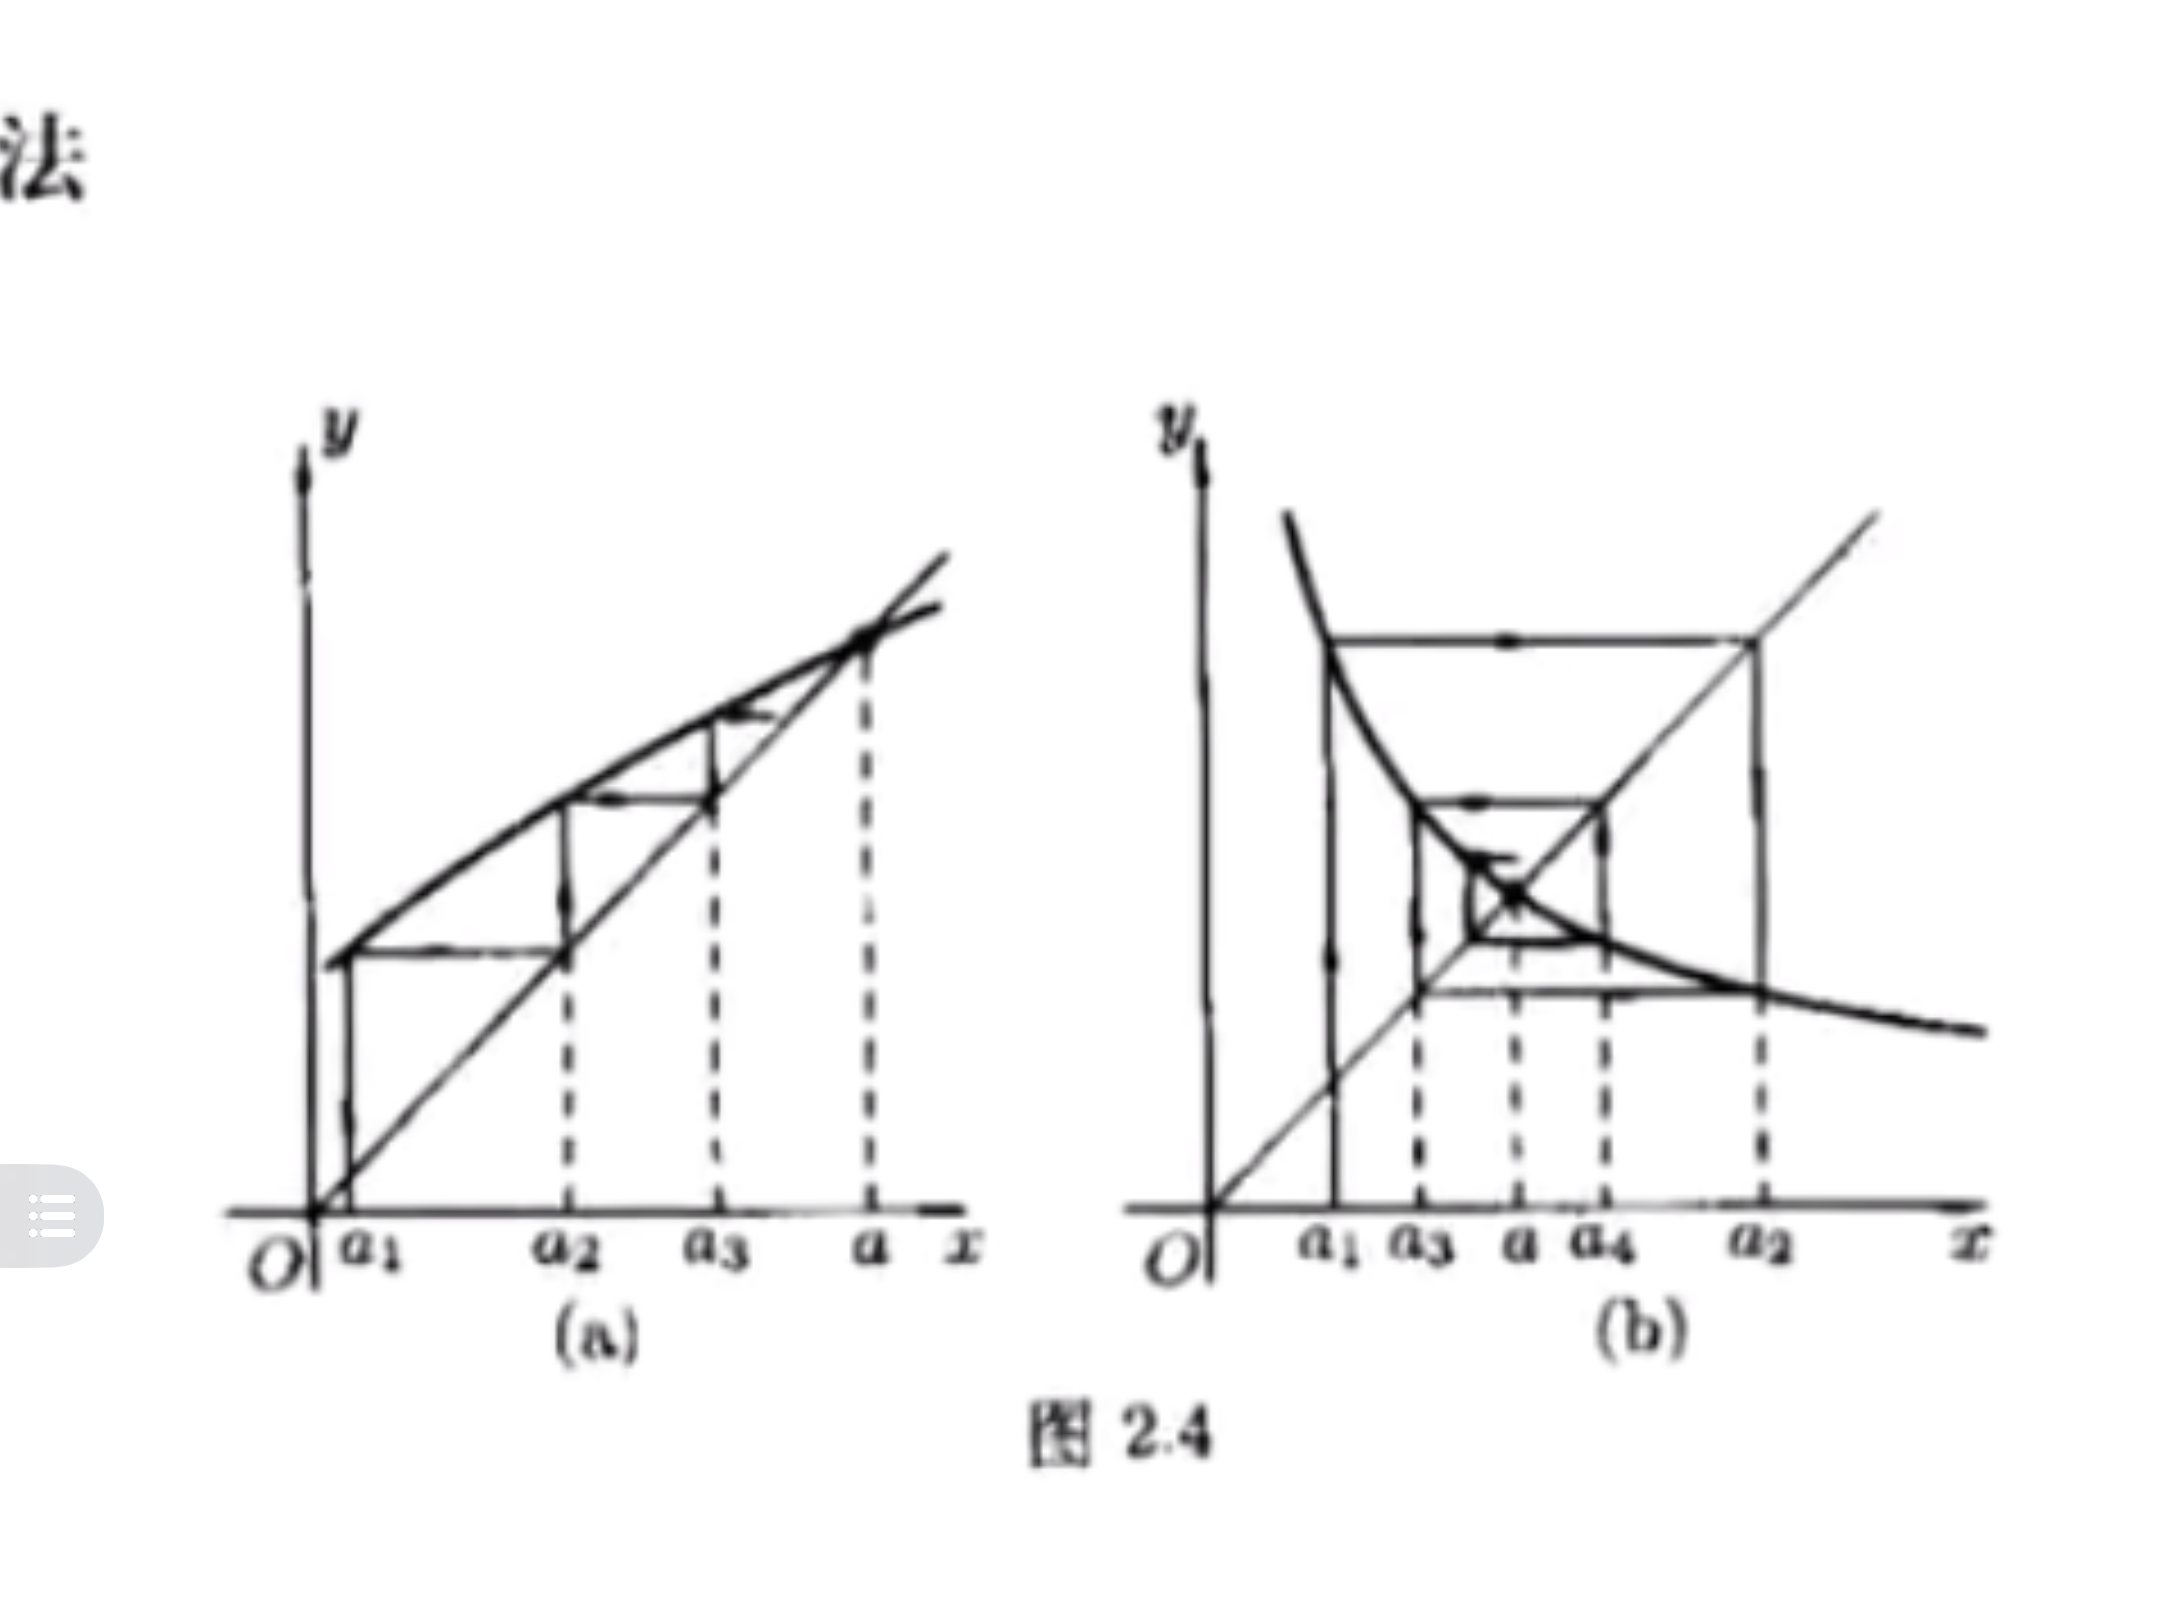
\includegraphics[width=0.5\textwidth]{figure/1.PNG}
\end{figure}
先看图2.4(a)。在其中的曲线代表函数 \( y = f(x) \)。它同直线 \( y = x \) 的交点的横坐标 \( a \) 就是 \( f \) 的不动点。从图中的 \( x \) 轴上代表初始值 \( a_1 \) 的点出发作平行于 \( y \) 轴的直线,它与曲线 \( y = f(x) \) 的交点的纵坐标就是 \( a_2 = f(a_1) \)。在这里的一个技巧是从上述交点作平行于 \( x \) 轴的直线与直线 \( y = x \) 相交。这个交点的横坐标当然也是 \( a_2 \)。在图中从这个交点作一条虚线与纵轴平行,并将它与 \( x \) 轴的交点标为 \( a_2 \)。这就完成了蛛网工作法的第一步。

在图2.4(a)上将这个方法继续做几步:可以看出,所得的数列是单调增加的

\begin{example}
	设 \( u_1 = b \), \( u_{n+1} = u_n^2 + (1 - 2a)u_n + a^2 \),试判断 \( u_n \) 的敛散性。
\end{example}
\begin{proof}
	折线图方法知当且仅当 $a-1 \le b \le a$ 时, $\lim_{n \to \infty} x_n$ 收敛且极限值为 $a$.
\end{proof}
\begin{example}
	设 \( x_{n+1}(2 - x_n) = 1 \), \( n = 1, 2, \cdots \)。试判断 \( x_n \) 的敛散性。
\end{example}
\begin{proof}
	折线图或者直接求通项的方法知 $\lim_{n \to \infty} x_n = 1$. 我们给出通项法证明:
    注意到由题目条件得
    $$
    x_n \ne 2, x_{n+1} - 1 = \frac{x_n - 1}{2 - x_n}, \quad n = 1, 2, \dots
    $$
    若 $x_{n_0} = 1$, 则 $x_n = 1, \forall n \ge n_0$, 此时当然有 $\lim_{n \to \infty} x_n = 1$. 因此下面假设 $x_n \ne 1, \forall n \ge 1$. 于是左右取倒数得
    $$
    \frac{1}{x_{n+1} - 1} = \frac{2 - x_n}{x_n - 1} = \frac{1}{x_n - 1} - 1 \implies \frac{1}{x_{n+1} - 1} - \frac{1}{x_n - 1} = -1 \implies \frac{1}{x_n - 1} = \frac{1}{x_1 - 1} - (n-1).
    $$
    % Note: The image derivation seems slightly different in the last step, showing:
    % \frac{1}{x_{n+1} - 1} = \frac{1}{x_1 - 1} - n \to -\infty
    因此 $\lim_{n \to \infty} x_{n+1} = 1$.
\end{proof}
\begin{example}
	定义数列 \( a_0 = x \), \( a_{n+1} = \frac{a_n^2 + y^2}{2} \), \( n = 0, 1, 2, \cdots \),记 \( D = \{(x, y) \in \mathbb{R}^2 : \text{数列 } a_n \text{ 收敛}\} \)。
\end{example}
\begin{proof}
	Step 1 \\
    $t = \frac{t^2+y^2}{2}$ 关于 $t$ 有解可知 $\Delta = 4 - 4y^2 \ge 0$, 即 $|y| \le 1$.

    Step 2 \\
    解 $t^2 - 2t + y^2 = 0$ 知 $t = 1 \pm \sqrt{1 - y^2}$, 由折线图技巧我们知道
    $$
    D = \{(x, y) \in \mathbb{R}^2 : 1 - \sqrt{1 - y^2} \le x \le 1 + \sqrt{1 - y^2}; |y| \le 1\}.
    $$
    % Note: The lower bound for x in the image looks like -1 - \sqrt{...}, but 1 - \sqrt{...} corresponds to the circle (x-1)^2 + y^2 = 1 derived from t = 1 +/- sqrt(1-y^2) if x=t. Using 1 - sqrt(...) as it seems contextually more likely.
    由初中数学得面积为 $4 + \pi$. % Note: The area of the domain D described above (a circle of radius 1) is \pi. The area 4+\pi might refer to a different context or shape.

\end{proof}
\chapter{函数}
\section{连续性和可微性}
\subsection{定义法}
\begin{example}
	(2023 复旦应统夏令营) 若 \( f'(x_0) \) 存在,试求 \(\lim_{h \to 0} \frac{f(x_0 + ah) - f(x_0 - bh)}{h}\);反之,若 \(\lim_{h \to 0} \frac{f(x_0 + h) - f(x_0) - h}{h}\) 存在,试问 \( f(x) \) 在 \( x_0 \) 处是否可导?
\end{example}
\begin{example}
	(2021 中科院考研) 若 \( f(x) \) 在 \( x = 0 \) 处连续,且 \(\lim_{x \to 0} \frac{f(2x) - f(x)}{x} = 0\),求证:\( f'(0) = 0 \)。
\end{example}
\begin{example}
	(2024 上交夏令营) 设函数 \( f(x) \) 在 \((-\infty, +\infty)\) 上连续,且 \(\lim_{x \to 0} \frac{f(x)}{x}\) 存在,令  
\[g(x) = \int_0^1 f(xt) \, dt,\]

(1) 求 \( g'(x) \);  

(2) 讨论 \( g'(x) \) 在 \( x=0 \) 处的连续性。
\end{example}
\subsection{级数法}
\begin{example}
	(2024 同济夏令营) 设 \(\{x_n\} \subset (0,1)\), \(x_j \neq x_i\) (\(i \neq j\)), 定义函数
\[ f(x) = \sum_{n=1}^{\infty} \frac{\operatorname{sgn}(x - x_n)}{2^n}, \]
试判断 \(f(x)\) 的连续性并给出证明。

\end{example}
\begin{example}
	(2023 复旦数科院夏令营) 设数列 \(\{r_n\}\) 为 \([0,1]\) 中的所有有理点的一个排列,证明函数
\[ f(x) = \sum_{n=1}^{\infty} \frac{|x - r_n|}{3^n}, \quad x \in [0,1] \]
具有以下性质:
\begin{enumerate}
    \item[(1)] 处处连续;
    \item[(2)] 在无理点处可微,有理点处不可微。
\end{enumerate}
\end{example}
\begin{example}
	(Cantor 函数) 设 \( C \) 为 \([0,1]\) 上的 Cantor 集,对于 \( x = 2 \sum_{i=1}^{\infty} \frac{a_i}{3^i} \in C \), \( a_i \in \{0,1\} \),令  
\[ \phi(x) = \phi\left(2 \sum_{i=1}^{\infty} \frac{a_i}{3^i}\right) = \sum_{i=1}^{\infty} \frac{a_i}{2^i}. \]  
Cantor 函数 \(\phi(x)\) 定义为:\(\forall x \in [0,1]\),  
\[ \phi(x) = \sup\{\phi(y) \mid y \in C, y \leq x\}. \]  
求证:\(\phi\) 为 \([0,1]\) 上的连续函数。
\end{example}
\begin{example}
	设 \( Q = \{x_1, x_2, \cdots\} \) 为有理数集合,令  
	\[ f(x) = \sum_{x_n \leq x} \frac{1}{2^n}, \]  
	证明:\( f(x) \) 仅在有理点处不连续。
\end{example}
\subsection{Schwarz导数}
\begin{definition}
	设有定义在开集 \( A \subset \mathbb{R} \) 上的实函数 \( f(x) \),若对于 \( a \in A \),
\[ \lim_{h \to 0} \frac{f(a+h)-f(a-h)}{2h} = f^s(a) \]
存在,则称 \( f(x) \) 在点 \( a \) Schwarz 可导,称 \( f^s(a) \) 为 Schwarz 导数。

\end{definition}
\begin{proposition}
	设 \( f(x) \in C[a,b] \) 且在 \( (a,b) \) 上 Schwarz 可导,那么:
\begin{itemize}
    \item 若 \( f(b) > f(a) \),则 \( \exists\, c \in (a,b) \),使得 \( f^s(c) \geq 0 \)。
    \item 若 \( f(a) > f(b) \),则 \( \exists\, c \in (a,b) \),使得 \( f^s(c) \leq 0 \)。
\end{itemize}

\end{proposition}
\begin{theorem}[Schwarz 导数的 Rolle 中值定理]
	设 \( f(x) \in C[a, b] \) 且在 \( (a, b) \) 上 Schwarz 可导,若 \( f(a) = f(b) \),则  
\(\exists\, r, t \in (a, b) \),使得 \( f^s(r) \geq 0 \) 且 \( f^s(t) \leq 0 \)。

\end{theorem}
\begin{theorem}[Schwarz 导数的 Lagrange 中值定理]
	设 \( f(x) \in C[a, b] \) 且在 \( (a, b) \) 上 Schwarz 可导,则存在 \( r, t \in (a, b) \),使得
\[ f^s(r) \leq \frac{f(b) - f(a)}{b - a} \leq f^s(t). \]
\end{theorem}
\begin{proof}
	和证明拉格朗日中值定理一样,我们只需证明罗尔中值定理的情况即可。即不妨设 $f(a) = f(b) = 0$,否则用 $F(x) - f(a) - \frac{f(b)-f(a)}{b-a}(x-a)$ 代替 $f$ 即可。
	
	若 $f \equiv 0$,则命题是显然的。若 $f$ 有正的最大值,则设 $c \in (a,b)$ 是 $f$ 的最大值点使得 $f(c)>0$,取 $k \in (0, f(c))$,构造非空有界集
	\[
	U = \{x \in [a,c] : f(x) > k\}.
	\]
	于是记 $x_1 = \inf U$,就有 $t_n \in U$,使得
	\[
	t_n \ge x_1, \lim_{n \to \infty} t_n = x_1.
	\]
	注意到 $x_1 \ne a$ 且若 $f(x_1) > k$,则由函数连续性知 $x_1$左侧仍有 $f>k$,这和 $x_1$ 是 $\inf$ 矛盾! 故我们只有 $x_1 \notin U$ 且 $f(x_1) = k$。
	现在
	\begin{align*}
	f^S(x_1) &= \lim_{h \to 0} \frac{f(x_1+h) - f(x_1-h)}{2h} = \lim_{n \to \infty} \frac{f(x_1+t_n-x_1) - f(x_1-(t_n-x_1))}{2(t_n-x_1)} \\
	&\ge \lim_{n \to \infty} \frac{k-k}{2(t_n-x_1)} = 0.
	\end{align*}
	若 $f$ 有负的最小值 $f(c)<0$. 取 $k \in (f(c), 0)$,构造非空有界集
	\[
	V = \{x \in [c,b]: f(x) < k\}.
	\]
	并取 $x_2 = \sup V$,同样的 $f(x_2)=k$ 且 $x_2 \ne b$. 存在 $s_n \in V$ 使得 $\lim_{n \to \infty} s_n = x_2$. 于是
	\begin{align*}
	f^S(x_2) &= \lim_{h \to 0} \frac{f(x_2+h) - f(x_2-h)}{2h} = \lim_{n \to \infty} \frac{f(x_2+s_n-x_2) - f(x_2-(s_n-x_2))}{2(s_n-x_2)} \\
	&\ge \lim_{n \to \infty} \frac{k-k}{2(s_n-x_2)} = 0.
	\end{align*}
	考虑 $f(a+b-x)$ 可得 $f^S(x_2)$, 这就完成了定理的证明。
	\end{proof}
	
\begin{theorem}[Schwarz 导数与一般导数的联系]
	设 \( f(x) \in C[a, b] \) 且在 \( (a, b) \) 上 Schwarz 可导,若 \( f^s(x) \) 在 \( (a, b) \) 上连续,则 \( f(x) \) 在 \( (a, b) \) 上可导且
\[ f'(x) = f^s(x), \quad \forall x \in (a, b). \]

\end{theorem}
\begin{proof}
	由 Schwarz 导数的 Lagrange 中值定理, 我们知道
	\[
	f^S(\theta_2) \ge \frac{f(x_2)-f(x_1)}{x_2-x_1} \ge f^S(\theta_1),
	\]
	且 $\theta_1, \theta_2$ 介于 $x_1, x_2$ 之间.
	
	让 $x_2 \to x_1$, 由 Schwartz 导数连续性和夹逼准则即可得
	\[
	f'(x_1) = f^S(x_1).
	\]
	这就完成了证明.
\end{proof}
\begin{theorem}[利用 Schwarz 导数判断函数单调性]
	设函数 \( f(x) \) 在开区间 \( I \) 上连续且 Schwarz 可导,若 \( f^s(x) \geq 0 \) 对所有 \( x \in I \) 成立,则 \( f(x) \) 在 \( I \) 上单调递增。
\end{theorem}
\begin{proof}
	对 $[c, d] \subset [a, b]$, 由 Schwarz 导数的 Lagrange 中值定理知存在 $\theta \in (c,d)$ 使得
\[
\frac{f(d)-f(c)}{d-c} \ge f^S(\theta) \ge 0,
\]
故
\[
f(d) \ge f(c).
\]
这就完成了证明.
\end{proof}
\section{一致连续性}
\begin{example}
	设 $f$ 定义在区间 $I$ 的函数. 证明 $f$ 在区间 $I$ 一致连续的充要条件是对任何 $\epsilon > 0$, 存在 $M > 0$, 使得对任何 $x_1, x_2 \in I$, 都有
	\[
	|f(x_2) - f(x_1)| \le M|x_1 - x_2| + \epsilon.
	\]
\end{example}
\begin{proof}
	\textbf{必要性:}因为 $f$ 一致连续, 所以对每个 $\epsilon > 0$, 存在 $\delta > 0$, 使得对任何 $x,y \in I$, 只要 $|x-y| \le \delta$, 就有
	\[
	|f(x)-f(y)| < \epsilon. 
	\]
	当 $|f(x)-f(y)| \le \epsilon$, 不等式然成立. 当 $|f(x)-f(y)| > \epsilon$, 不妨设 $y>x, f(y)>f(x)$ 且令 $f(y)-f(x) = kt, k \in \mathbb{N}, t \in (\epsilon, 2\epsilon]$. 由介值定理, 存在 $x=x_0 < x_1 < \dots < x_k = y$ 使得
	\[
	f(x_j) = f(x) + jt, j=0, 1, 2, \dots, k.
	\]
	于是
	\[
	f(x_j) - f(x_{j-1}) = t > \epsilon, j=1, 2, \dots, k,
	\]
	易知 $x_j - x_{j-1} > \delta, j=1, 2, \dots, k$. 从而我们有
	\[
	y-x = \sum_{j=1}^k (x_j - x_{j-1}) > k\delta.
	\]
	现在可取 $M=\frac{2\epsilon}{\delta} > 0$, 于是就有
	\[
	|f(y)-f(x)| = kt \le \frac{t}{\delta}|y-x| \le \frac{2\epsilon}{\delta}|y-x| = M|y-x|.
	\]
	这就证明了不等式成立.
	
	\textbf{充分性:}对任何 $\epsilon > 0$, 存在 $M>0$, 使得对任何 $x_1, x_2 \in I$, 都有(12.49)成立. 于是取 $\delta = \frac{\epsilon}{M}>0$, 当 $x,y \in I, |x-y|\le \delta$, 我们就有
	\[
	|f(x)-f(y)| \le 2\epsilon,
	\]
	这就证明了 $f$ 在 $I$ 上一致连续.
	\end{proof}
	
\begin{example}
	设 \( f(x) \) 在 \([a, +\infty)\) 上一致连续,\( g(x) \) 在 \([a, +\infty)\) 上连续,且
\[ \lim_{x \to +\infty} |f(x) - g(x)| = 0. \]
求证:\( g(x) \) 在 \([a, +\infty)\) 上一致连续。
\end{example}
\begin{example}
	设 \( f(x) \) 在 \([1, +\infty)\) 上一致连续。求证:存在 \( M > 0 \),使得
\[ \frac{|f(x)|}{x} \leq M, \quad \forall x \in [1, +\infty). \]
\end{example}
\begin{proof}
	在例题2.8中取 $x_2 = x, x_1=1, \epsilon = 1$ 知存在 $c>0$ 使得
\[
|f(x)-f(1)| \le c|x-1|+1, \forall x \ge 1.
\]
于是
\[
\left|\frac{f(x)}{x}\right| \le \left|\frac{f(x)-f(1)}{x}\right| + \left|\frac{f(1)}{x}\right| \le c\left|1-\frac{1}{x}\right| + \frac{1+|f(1)|}{x}.
\]
注意到
\[
\varlimsup_{x \to +\infty} \left|\frac{f(x)}{x}\right| \le \varlimsup_{x \to +\infty} \left[ c\left|1-\frac{1}{x}\right| + \frac{1+|f(1)|}{x} \right] = c,
\]
于是我们知道存在 $M>0$ 使得
\[
\left|\frac{f(x)}{x}\right| \le M, \forall x \ge 1.
\]
\end{proof}
\begin{example}
	设 \( f(x) \) 在 \([0, +\infty)\) 上一致连续,且对任意 \( x \geq 0 \) 有
\[ \lim_{n \to +\infty} f(x+n) = 0, \quad n \in \mathbb{N}. \]
求证:
\[ \lim_{x \to +\infty} f(x) = 0. \]
\end{example}
\begin{example}
	设 \( f(x) \) 在 \([0, +\infty)\) 上连续,且满足
\[ \lim_{n \to \infty} f(\sqrt{n}) = 0. \]
求证:\(\lim_{x \to +\infty} f(x)\) 存在当且仅当 \( f(x) \) 在 \([0, +\infty)\) 上一致连续。

\end{example}
\begin{example}
	若 \( f(x) \) 在 \([0,+\infty)\) 上可导,且满足:
\begin{enumerate}
    \item \( f'(x) \) 在 \([0,+\infty)\) 上一致连续;
    \item \( \lim_{x \to +\infty} f(x) \) 存在。
\end{enumerate}
求证:
\[ \lim_{x \to +\infty} f'(x) = 0. \]
\end{example}
\begin{example}
	(2024 国防科大考研) 设函数 \( f(x) \) 在 \( (0,1] \) 上连续且可导,且满足
    \[ \lim_{x \to 0^+} \sqrt{x}f'(x) = a. \]
    求证:\( f(x) \) 在 \( (0,1] \) 上一致连续。
\end{example}
\begin{proof}
	首先 $\int_0^a \frac{1}{\sqrt{x}}dx$ 收敛且收敛必有界知
\[
\sup_{y \in (0, a]} |\sqrt{y}f'(y)| < +\infty.
\]
设 $a \ge x_2 > x_1 > 0$, 则由
\[
f(x_2) - f(x_1) = \int_{x_1}^{x_2} f'(y) \, dy = \int_{x_1}^{x_2} \sqrt{y}f'(y) \frac{1}{\sqrt{y}} \, dy \le \sup_{y \in (0, a]} |\sqrt{y}f'(y)| \int_{x_2}^{x_1} \frac{1}{\sqrt{y}} \, dy
\]
和 Cauchy 收敛准则知 $\lim_{x \to 0^+} f(x)$ 存在. 由 Cantor 定理知 $f$ 在 $[0, a]$ 一致连续.

\end{proof}
\begin{example}
	(2024 哈工大考研) 设 \( (a,b) \) 为有界开区间,求证:\( f(x) \) 在 \( (a,b) \) 上一致连续的充要条件是对于任意 Cauchy 列 \( \{x_n\} \subset (a,b) \),像列 \( \{f(x_n)\} \) 也是 Cauchy 列。
\end{example}
\begin{example}
	(2023 吉大夏令营) 设 \( f(x) \in C[1,+\infty) \),且满足
    \[ \lim_{x \to +\infty} \frac{f(x)}{x^2} = 1. \]
    求证:\( f(x) \) 在 \( [1,+\infty) \) 上非一致连续。
\end{example}
\section{函数方程}
\subsection{柯西方程}
\begin{definition}
	我们称函数 \( f \colon \mathbb{R} \to \mathbb{R} \) 满足的函数方程
\[ f(x + y) = f(x) + f(y) \]
为 \textbf{Cauchy 方程}。
\end{definition}
\begin{example}
	设 \( f \colon \mathbb{R} \to \mathbb{R} \) 是 Cauchy 方程的解,则:
\begin{enumerate}
    \item[(1)] 对任意有理数 \( r \in \mathbb{Q} \),有
    \[ f(rx) = r f(x); \]
    \item[(2)] 进一步,若 \( f \) 连续,则存在常数 \( c = f(1) \) 使得
    \[ f(x) = c x, \quad \forall x \in \mathbb{R}. \]
\end{enumerate}
\end{example}
\begin{proof}
	\begin{enumerate}
		\item \textbf{Step 1} 注意到 $f(2x) = f(x+x) = f(x) + f(x) = 2f(x)$, 然后
		\[
		f(3x) = f(2x+x) = f(2x)+f(x) = 2f(x)+f(x) = 3f(x).
		\]
		依次下去可得
		\[
		f(nx) = nf(x), \forall n \in \mathbb{N}.
		\]
		
		\noindent\textbf{Step 2} 现在对每个 $r = \frac{p}{q} \in \mathbb{Q}, q \neq 0$, 我们注意到
		\[
		rf(x) = f(rx) \iff pf(x) = qf\left(\frac{p}{q}x\right).
		\]
		现在反复运用上式, 我们知道
		\[
		qf\left(\frac{p}{q}x\right) = f(px) = pf(x).
		\]
.
		\item 对每个无理数 $r$,存在有理数列 $r_n, n=1, 2, \cdots$ 使得 $\lim_{n\to\infty} r_n = r$。我们知道
		\[
		f(rx) = \lim_{n\to\infty} f(r_n x) = \lim_{n\to\infty} r_n f(x) = r f(x).
		\]

	\end{enumerate}
\end{proof}
\begin{example}
	求证:\(\mathbb{R}\) 上既凸又凹的连续函数必为线性函数,即存在常数 \( a, b \in \mathbb{R} \) 使得
\[ f(x) = a x + b, \quad \forall x \in \mathbb{R}. \]
\end{example}

\begin{remark}
	容易由证明知道任何开区间 $(a, b)$ 上的既凸又凹的连续函数也是直线。
\end{remark}

\begin{proof}
	注意到
\[
f\left(\frac{x+y}{2}\right) = \frac{1}{2}f(x) + \frac{1}{2}f(y).
\]
考虑 $g(x) = f(x) - f(0)$, 则运用 $f(x+y)+f(0) = 2f(\frac{x+y}{2})$ 知 $g$ 满足 Cauchy 方程11.7. 于是我们知道
\[
f(x) = f(0) + [f(1) - f(0)]x.
\]

\end{proof}
\begin{example}
	设 \( f(x) \) 在 \( (0, +\infty) \) 上连续,且满足函数方程:
\[ f(xy) = x f(y) + y f(x), \quad \forall x, y \in (0, +\infty). \]
求证:\( f(x) \) 在 \( (0, +\infty) \) 上可微。
\end{example}
\begin{proof}
	首先
\[
f(0) = xf(0), \forall x \in \mathbb{R} \Rightarrow f(0) = 0, \quad f(x) = xf(1) + f(x), \forall x \in \mathbb{R} \Rightarrow f(1) = 0.
\]

\noindent 现在
\[
f(-x) = xf(-1) - f(x), f(x) = -xf(-1) - f(-x) \Rightarrow 2xf(-1)=0 \Rightarrow f(-1)=0.
\]

\noindent 于是
\[
f(-x) = xf(-1) - f(x) = -f(x),
\]

\noindent 即 $f$ 是奇函数。

\noindent 对 $x, y > 0$, 取 $x=e^s, y=e^t, s, t \in (-\infty, +\infty)$, 我们有
\[
\frac{f(e^{s+t})}{e^{s+t}} = \frac{f(e^s)}{e^s} + \frac{f(e^t)}{e^t},
\]

\noindent 即 $\frac{f(e^x)}{e^x}$ 满足 Cauchy 方程11.7. 因此
\[
\frac{f(e^x)}{e^x} = \frac{f(e)}{e}x, \forall x \in \mathbb{R}.
\]

\noindent 现在可得
\[
f(x) = 
\begin{cases}
    \frac{f(e)}{e} x \ln x, & x > 0 \\
    0, & x=0 \\
    \frac{f(e)}{e} x \ln(-x), & x < 0
\end{cases}.
\]

结论显然成立
\end{proof}
\begin{example}
	(2024 中科院夏令营) 证明:在 \( \mathbb{R} \) 上满足函数方程
\[ f(x+y) = f(x) f(y) \]
的唯一不恒等于零的连续解是指数函数 \( f(x) = a^x \),其中 \( a > 0 \) 为常数。
\end{example}
\begin{proof}
		首先,若存在一点 $x_0$ 使得 $f(x_0)=0$,则对任意 $x \in \mathbb{R}$,有 $f(x) = f(x-x_0+x_0) = f(x-x_0)f(x_0)=0$。这导致 $f(x) \equiv 0$,此为平凡解。因我们寻找非平凡解,故可设 $f(x) \neq 0, \forall x \in \mathbb{R}$。
		
		于是,对任意 $x \in \mathbb{R}$,$f(x) = f(\frac{x}{2}+\frac{x}{2}) = \left(f(\frac{x}{2})\right)^2 \ge 0$。结合 $f(x) \neq 0$,可知 $f(x) > 0$。
		在原方程中令 $y=0$,得 $f(x) = f(x)f(0)$。因为 $f(x)>0$,两边消去 $f(x)$ 得 $f(0)=1$。
		
		证明过程分三步:
		\begin{enumerate}
			\item \textbf{证明对整数成立} \\
			令 $a = f(1)$。由于 $f(x)>0$,$a>0$。
			对任意正整数 $n \in \mathbb{N}$,通过归纳法可得 $f(n) = f(1+\dots+1) = (f(1))^n = a^n$。
			对负整数 $-n$,$1 = f(0) = f(n+(-n)) = f(n)f(-n) = a^n f(-n)$,故 $f(-n) = a^{-n}$。
			因此,对所有整数 $k \in \mathbb{Z}$,均有 $f(k) = a^k$。
		
			\item \textbf{证明对有理数成立} \\
			设 $x = \frac{p}{q}$ 是任意有理数,其中 $p, q \in \mathbb{Z}, q \neq 0$。
			根据第1步的结论,我们有:
			\[
			a^p = f(p) = f\left(q \cdot \frac{p}{q}\right) = \left(f\left(\frac{p}{q}\right)\right)^q.
			\]
			由于 $f(x)>0, a>0$,两边开 $q$ 次方,得 $f(\frac{p}{q}) = (a^p)^{\frac{1}{q}} = a^{\frac{p}{q}}$。
			因此,对所有有理数 $x \in \mathbb{Q}$,均有 $f(x) = a^x$。
		
			\item \textbf{证明对实数成立} \\
			对任意实数 $x \in \mathbb{R}$,存在一个有理数序列 $\{q_n\}_{n=1}^\infty$ 使得 $\lim_{n\to\infty} q_n = x$。
			由于函数 $f(x)$ 和指数函数 $g(x)=a^x$ 均是连续函数,我们有:
			\[
			f(x) = f\left(\lim_{n\to\infty} q_n\right) = \lim_{n\to\infty} f(q_n).
			\]
			根据第2步的结论,$f(q_n) = a^{q_n}$,所以
			\[
			f(x) = \lim_{n\to\infty} a^{q_n} = a^{\lim_{n\to\infty} q_n} = a^x.
			\]
			这就证明了 $f(x) = a^x$ 对所有 $x \in \mathbb{R}$ 成立,其中 $a=f(1)>0$ 是一个常数。
		\end{enumerate}
\end{proof}
\subsection{迭代法}
\textbf{基本思想}:通过构造递推关系,将函数方程转化为可求和的形式。
\begin{example}
	求函数方程 
\[ 2f(2x) = f(x) + x \]
在 $\mathbb{R}$ 上且满足 $f$ 在 $x=0$ 处连续的所有解。
\end{example}
\begin{proof}
	注意到
\[
\frac{1}{2^n}f\left(\frac{x}{2^n}\right) = \frac{1}{2^{n+1}}f\left(\frac{x}{2^{n+1}}\right) + \frac{x}{2^{2n+2}}, \quad n=0, 1, 2, \dots
\]

\noindent
于是
\begin{align*}
f(x) - \lim_{n\to\infty}\frac{1}{2^{n+1}}f\left(\frac{x}{2^{n+1}}\right) 
&= \sum_{n=0}^{\infty} \left[ \frac{1}{2^n}f\left(\frac{x}{2^n}\right) - \frac{1}{2^{n+1}}f\left(\frac{x}{2^{n+1}}\right) \right] \\
&= \sum_{n=0}^{\infty} \frac{x}{2^{2n+2}} = \frac{1}{4}x \cdot \frac{1}{1-\frac{1}{4}} = \frac{x}{3}.
\end{align*}

\noindent
因此结合 $f(0)=0$ 知 $f(x) = \frac{x}{3}$.
\end{proof}
\begin{example}
	求函数方程
\[ f(x+y) - f(x-y) = f(x)f(y) \]
在 $\mathbb{R}$ 上且满足 $f$ 在 $x=0$ 处连续的所有解。
\end{example}
\begin{proof}
	取 $y=x$, 于是 $f(2x)-f(0)=f^2(x)$, 令 $x=0$ 知 $f(0)=0$. 现在考虑 $f(2x) = f^2(x) \ge 0$, 即 $f$ 是非负函数. 注意到对每个 $n \in \mathbb{N}$, 我们有
\begin{equation}
f(x) = f^{2}\left(\frac{x}{2}\right) = f^{2^2}\left(\frac{x}{2^2}\right) = \cdots = f^{2^n}\left(\frac{x}{2^n}\right). 
\end{equation}
于是,令 $n \to \infty$ 并结合 $f$ 在 $x=0$ 连续性我们有
\[
f(x) = \lim_{n\to\infty} f^{2^n}\left(\frac{x}{2^n}\right) = 0.
\]
\end{proof}
\begin{example}
	求函数方程 
    \[ f(\log_2 x) = f(\log_3 x) + \log_5 x \]
    在 \( \mathbb{R}^+ \) 上的所有连续解。
\end{example}
\begin{proof}
	取
\[
a_1 = x, \ln a_n = \left(\frac{\ln 2}{\ln 3}\right)^{n-1} \ln x, n \in \mathbb{N}.
\]

\noindent
现在
\[
f\left(\frac{\ln a_n}{\ln 2}\right) = f\left(\frac{\ln a_{n+1}}{\ln 2}\right) + \frac{\ln a_n}{\ln 5}, \quad n = 1, 2, \dots,
\]

\noindent
于是
\begin{align*}
\sum_{n=1}^{\infty} \left[ f\left(\frac{\ln a_n}{\ln 2}\right) - f\left(\frac{\ln a_{n+1}}{\ln 2}\right) \right] 
&= \sum_{n=1}^{\infty} \frac{\ln a_n}{\ln 5} \\
&= \sum_{n=1}^{\infty} \left(\frac{\ln 2}{\ln 3}\right)^{n-1} \frac{\ln x}{\ln 5} \\
&= \frac{\ln x}{\ln 5} \frac{\ln 3}{\ln 3 - \ln 2}.
\end{align*}

结合
\begin{align*}
\sum_{n=1}^{\infty} \left[ f\left(\frac{\ln a_n}{\ln 2}\right) - f\left(\frac{\ln a_{n+1}}{\ln 2}\right) \right] 
&= f\left(\frac{\ln a_1}{\ln 2}\right) - \lim_{n\to\infty} f\left(\frac{\ln a_{n+1}}{\ln 2}\right) \\
&= f\left(\frac{\ln x}{\ln 2}\right) - f(0),
\end{align*}

\noindent
我们知道
\[
f(x) = f(0) + \frac{x \ln 2 \ln 3}{\ln 5 \ln \frac{3}{2}}.
\]
\end{proof}
\chapter{一元函数微分学}
\section{微分中值定理}
\subsection{插值法}
有一类中值定理习题中往往会给我们很多关于函数 $f(x)$ 的信息,进而去证明一个等式。如何利用好这些已知信息?这就涉及到数值分析中的 Lagrange 插值与 Newton 插值。
\begin{theorem}[Lagrange 插值]
	已知插值节点为 $(x_i, y_i), i = 0, 1, 2, \cdots, n$,那么

\[ y = f(x) = \sum_{0 \leq i < n} \frac{(x - x_0) \cdots (x - x_{i-1})(x - x_{i+1}) \cdots (x - x_n)}{(x_i - x_0) \cdots (x_i - x_{i-1})(x_i - x_{i+1}) \cdots (x_i - x_n)} y_i \]

对应的插值余项为:

\[ R_n(x) = f(x) - L_n(x) = \frac{f^{(n+1)}(\xi)}{(n+1)!}(x - x_0)(x - x_1) \cdots (x - x_n) \]

\end{theorem}
\begin{theorem}[Newton 插值]
	已知插值节点为 $(x_i, y_i), i = 0, 1, 2, \cdots, n$,那么

\[ f(x) = a_0 + a_1(x - x_0) + a_2(x - x_0)(x - x_1) + \cdots + a_n(x - x_0)(x - x_1)(x - x_2) \cdots (x - x_{n-1}), \]

其中 $a_n = f[x_0, x_1, \cdots, x_k]$,对应的插值余项为:

\[ R_n(x) = f(x) - L_n(x) = \frac{f^{(n+1)}(\xi)}{(n+1)!}(x - x_0)(x - x_1) \cdots (x - x_n) \]

\textbf{Tip:} Newton 插值可以带重节点,进而反映出导数信息。
\end{theorem}
\begin{example}
	设 $f \in D^3[-1, 1]$,$f(-1) = 0$,$f'(0) = 0$,$f(1) = 1$。求证:$\exists \theta \in (-1, 1)$,s.t. $f'''(\theta) = 3$。
\end{example}

\begin{remark}
	本题拟和 $f(-1), f(1), f(0), f'(0), 4$ 个条件暗含插值多项式 3 次, 余项应该到 4 阶导, 条件只有 3 阶导, 因此本题是一种新的模型. 即 $f'''(\theta) = p'''(\theta)$ 这种模型.

\end{remark}
\begin{proof}
	设
\[
p(x) = \frac{(x-0)(x-1)}{(-1-0)(-1-1)}f(-1) + \frac{(x+1)(x-1)}{(0+1)(0-1)}f(0) + \frac{(x+1)(x-0)}{(1+1)(1-0)}f(1) + cx(x+1)(x-1).
\]
代入导数条件得 $c = \frac{1}{2}$.

注意到 $F(x) = f(x) - p(x)$ 满足
\begin{equation}
F(0) = F(1) = F(-1) = F'(0) = 0. \tag{10.9}
\end{equation}
对 $F$ 反复使用罗尔中值定理知存在 $\theta \in (-1, 1)$, 使得 $F'''(\theta)=0$, 直接计算表明
\begin{equation}
F'''(\theta) = f'''(\theta) - p'''(\theta) = f'''(\theta) - \frac{1}{2} \cdot 3! = 0
\end{equation}

\end{proof}
\begin{example}
	设 \(f \in C[0, 2] \cap D(0, 2)\) 满足 \(f(0) = f(2) = 0\), \(|f'(x)| \leq M\), \(\forall x \in (0, 2)\)。求证:
\[ \left| \int_{0}^{2} f(x) \, dx \right| \leq M. \]
\end{example}

\begin{remark}
	插 $f(0), f(2)$, 插值多项式 1 次, 余项 2 阶, 导数不够, 属于靠近哪边对哪边插模型.
\end{remark}
\begin{proof}
	当 $x \in [0, 1]$, 由插值定理, 我们有
\[
f(x) = f(0) + \frac{f'(\theta(x))}{1!}(x-0) = f'(\theta(x))x,
\]
于是
\[
|f(x)| \le |f'(\theta(x))| \cdot x \le Mx.
\]
当 $x \in [1, 2]$, 由插值定理, 我们有
\[
f(x) = f(2) + \frac{f'(\zeta(x))}{1!}(x-2) = f'(\zeta(x))(x-2),
\]
于是
\[
|f(x)| \le |f'(\zeta(x))| \cdot |x-2| \le M(2-x).
\]
结合上式, 我们有
\begin{align*}
    \left| \int_0^2 f(x) \,dx \right| &\le \int_0^2 |f(x)| \,dx = \int_0^1 |f(x)| \,dx + \int_1^2 |f(x)| \,dx \\
    &\le \int_0^1 (Mx) \,dx + \int_1^2 (M(2-x)) \,dx \\
    &= M.
\end{align*}

\end{proof}
\begin{example}
	设 \( f \in C^3[0,2] \) 满足
\[ f(0) = f'(0) = 0, \quad \int_{0}^{2} f(x) \, dx = 8 \int_{0}^{1} f(x) \, dx. \]
证明:存在 \( \theta \in (0,2) \),使得 \( f''(\theta) = 0 \)。
\end{example}

\begin{remark}
	考虑 $F(x) = \int_0^x f(y) \, dy \in C^4[0, 2]$, 初值条件即
\[
F(0) = F'(0) = F''(0) = 0, F(2) = 8F(1).
\]
这里插点 $F(1), F(2), F(0), F'(0), F''(0)$, 合计 5 个条件, 插值多项式 4 次, 余项 5 阶, 条件不够, 属于模型 $F'''' = p''''$.

\end{remark}

\begin{proof}
	为确定 $p$, 注意到 0 是 $p$ 的三重零点, 考虑 $p(x) = x^3(ax+b)$, 则
\[
F(2) = 8F(1) \Rightarrow p(2) = 8p(1) \Rightarrow a=0,
\]
即 $p(x) = F(1)x^3$. 由插值定理10.1, 存在 $\theta \in (0, 2)$, 使得
\[
f'''(\theta) = F''''(\theta) = p''''(\theta) = 0.
\]
这就完成了证明.

\end{proof}
下面我们来介绍插值法的积分型余项,这种余项往往蕴含着更多的信息。
\begin{theorem}[积分型余项]
	设 \( f(x) \) 是 \([a,b]\) 上的二阶可导函数且 \( f''(x) \in R[a,b] \),则有:
\[ f(x) = \frac{b-x}{b-a}f(a) + \frac{x-a}{b-a}f(b) + \int_a^b f''(y)k(x,y)dy, \]
其中,
\[ k(x,y) = 
\begin{cases} 
\frac{(x-a)(y-b)}{b-a}, & a \leq y \leq x \leq b; \\ 
\frac{(b-x)(a-y)}{b-a}, & a \leq x \leq y \leq b.
\end{cases} \]
\end{theorem}
\begin{example}
	(2021华东师范考研压轴) 设 \( f \in C^2[0,1] \) 满足 \( f(0) = f(1) = 0 \),证明:
\[ \int_0^1 \left| \frac{f''(x)}{f(x)} \right| dx \geq 4. \]
\end{example}

\begin{remark}
	我们指出不等式中的 4 是最佳的. 从下述证明可以看到放缩核心是
\[
|k(x, y)| \le k(x, x) \le k\left(\frac{1}{2}, \frac{1}{2}\right) = \frac{1}{4}.
\]
因此我们期望 $f''$ 其中在 $x=\frac{1}{2}$ 附近且值为 1. 于是考虑
\[
f_n(x) = 
\begin{cases}
    \frac{n^3}{8} \left(x - \frac{1}{2}\right)^4 - \frac{3n}{4} \left(x - \frac{1}{2}\right)^2 + \frac{4n-3}{8n}, & x \in \left[\frac{1}{2} - \frac{1}{n}, \frac{1}{2} + \frac{1}{n}\right] \\
    x, & x \in \left[0, \frac{1}{2} - \frac{1}{n}\right) \\
    -(x-1), & x \in \left(\frac{1}{2} + \frac{1}{n}, 1\right]
\end{cases}
, n \ge 2.
\]
由于
\[
f_n''(x) \le 0, x \in \left[\frac{1}{2} - \frac{1}{n}, \frac{1}{2} + \frac{1}{n}\right], f_n(x) \ge 0, x \in [0, 1],
\]
我们有
\begin{align*}
\int_0^1 \frac{|f_n''(x)|}{f_n(x)} \, dx &= -\int_{\frac{1}{2}-\frac{1}{n}}^{\frac{1}{2}+\frac{1}{n}} \frac{f_n''(x)}{f_n(x)} \, dx \quad \overset{\text{积分中值定理}}{=} -\frac{1}{f_n(\xi_n)} \int_{\frac{1}{2}-\frac{1}{n}}^{\frac{1}{2}+\frac{1}{n}} f_n''(x) \, dx \left(\xi_n - \frac{1}{2} < \frac{1}{n}\right) \\
&= \frac{2}{f_n(\xi_n)} = \frac{2}{n^3(\xi_n - \frac{1}{2})^4 - 3n(\xi_n - \frac{1}{2})^2 + \frac{4n-3}{n}} \to 4, n \to \infty.
\end{align*}
\end{remark}
\begin{proof}
	事实上, 我们知道
\[
f(x) = \int_0^1 f''(y) k(x, y) \, dy.
\]
于是利用
\[
|k(x, y)| \le |k(x, x)| = x(1-x),
\]
就有
\[
|f(x)| \le \int_0^1 |k(x,y)| \cdot |f''(y)| \, dy \le x(1-x) \int_0^1 |f''(y)| \, dy \le \frac{1}{4} \int_0^1 |f''(y)| \, dy,
\]
从而
\[
\int_0^1 \frac{|f''(x)|}{f(x)} \, dx \ge \int_0^1 \frac{|f''(x)|}{\frac{1}{4} \int_0^1 |f''(y)| \, dy} \, dx = 4.
\]
这就完成了证明.
\end{proof}
\begin{example}
	设 \( f(x) \in D^2[0, 1] \), \( f(0) = f(1) = 0 \), \( |f''(x)| \leq M \), 求证:
    \[ \int_{0}^{1} f(x) \, dx \leq \frac{M}{12} \]
    
\end{example}
\begin{proof}
    事实上, 对于满足边界条件 $f(0)=f(1)=0$ 的函数, 我们可以利用格林函数将其表示为
    \[
    f(x) = \int_0^1 k(x,y) f''(y) \, dy,
    \]
    其中核函数(格林函数)为
    \[
    k(x,y) = 
    \begin{cases}
        y(x-1), & 0 \le y \le x \\
        x(y-1), & x \le y \le 1
    \end{cases}
    .
    \]
    于是, 我们对 $f(x)$ 进行积分
    \[
    \int_0^1 f(x) \, dx = \int_0^1 \left( \int_0^1 k(x,y) f''(y) \, dy \right) dx.
    \]
    通过交换积分次序 (Fubini 定理), 我们得到
    \[
    \int_0^1 f(x) \, dx = \int_0^1 f''(y) \left( \int_0^1 k(x,y) \, dx \right) dy.
    \]
    我们先计算内层关于 $x$ 的积分:
    \begin{align*}
        \int_0^1 k(x,y) \, dx &= \int_0^y x(y-1) \, dx + \int_y^1 y(x-1) \, dx \\
        &= (y-1) \left[ \frac{x^2}{2} \right]_0^y + y \left[ \frac{x^2}{2} - x \right]_y^1 \\
        &= (y-1)\frac{y^2}{2} + y \left( (\frac{1}{2} - 1) - (\frac{y^2}{2} - y) \right) \\
        &= \frac{y^3-y^2}{2} + y \left( -\frac{1}{2} - \frac{y^2}{2} + y \right) \\
        &= \frac{y^3-y^2}{2} - \frac{y}{2} - \frac{y^3}{2} + y^2 = \frac{y^2-y}{2}.
    \end{align*}
    将此结果代回, 就有
    \[
    \int_0^1 f(x) \, dx = \int_0^1 f''(y) \frac{y^2-y}{2} \, dy.
    \]
    从而, 利用已知条件 $|f''(y)| \le M$,
    \begin{align*}
        \left| \int_0^1 f(x) \, dx \right| &= \left| \int_0^1 f''(y) \frac{y^2-y}{2} \, dy \right| \\
        &\le \int_0^1 |f''(y)| \left| \frac{y^2-y}{2} \right| \, dy \\
        &\le M \int_0^1 \frac{y-y^2}{2} \, dy \\
        &= \frac{M}{2} \left[ \frac{y^2}{2} - \frac{y^3}{3} \right]_0^1 = \frac{M}{2} \left( \frac{1}{2} - \frac{1}{3} \right) = \frac{M}{12}.
    \end{align*}
    因为 $\int_0^1 f(x) \, dx \le \left|\int_0^1 f(x) \, dx\right|$, 所以原命题成立. 这就完成了证明.
\end{proof}
\begin{example}
	已知 \( f(x) \in C^2[a, b] \), \( f(a) = f(b) = 0 \), 求证:
    \[ |f(x)| \leq \frac{(x - a)(b - x)}{b - a} \int_{a}^{b} |f''(y)| \, dy \]
\end{example}
\begin{proof}
    事实上, 我们知道对于满足边界条件 $f(a)=f(b)=0$ 的函数, 有如下格林函数表示:
    \[
    f(x) = \int_a^b k(x,y) f''(y) \, dy,
    \]
    其中核函数 $k(x,y)$ 为
    \[
    k(x,y) = \frac{1}{b-a}
    \begin{cases}
        (y-a)(x-b), & a \le y \le x \\
        (x-a)(y-b), & x \le y \le b
    \end{cases}
    .
    \]
    于是利用绝对值不等式,
    \[
    |f(x)| = \left| \int_a^b k(x,y) f''(y) \, dy \right| \le \int_a^b |k(x,y)| |f''(y)| \, dy.
    \]
    我们来考察核函数 $|k(x,y)|$. 对于固定的 $x \in [a,b]$:
    \begin{itemize}
        \item 当 $a \le y \le x$ 时, $y-a \ge 0$, $x-b \le 0$, 故
        \[ |k(x,y)| = \frac{(y-a)(b-x)}{b-a} \le \frac{(x-a)(b-x)}{b-a}. \]
        \item 当 $x \le y \le b$ 时, $x-a \ge 0$, $y-b \le 0$, 故
        \[ |k(x,y)| = \frac{(x-a)(b-y)}{b-a} \le \frac{(x-a)(b-x)}{b-a}. \]
    \end{itemize}
    因此, 对所有的 $y \in [a,b]$, 我们有一致的界:
    \[
    |k(x,y)| \le \frac{(x-a)(b-x)}{b-a}.
    \]
    从而, 将此不等式代入积分, 就有
    \begin{align*}
        |f(x)| &\le \int_a^b |k(x,y)| |f''(y)| \, dy \\
        &\le \int_a^b \frac{(x-a)(b-x)}{b-a} |f''(y)| \, dy \\
        &= \frac{(x-a)(b-x)}{b-a} \int_a^b |f''(y)| \, dy.
    \end{align*}
    这就完成了证明.
\end{proof}
\subsection{K值法}
看例题操作,有手就行
\begin{example}
	(2021 天津大学考研) 设函数 \( f(x) \in C[a,b] \cap D^2(a,b) \),求证:\(\exists \xi \in (a,b)\),使得
\[ f(b) - 2f\left(\frac{a+b}{2}\right) + f(a) = \frac{(b-a)^2}{4}f''(\xi). \]
\end{example}
\begin{proof}
    事实上, 记常数 $K$ 满足
\[
f(b) - 2f\left(\frac{a+b}{2}\right) + f(a) = \frac{(b-a)^2}{4}K.
\]
即
\[
K = \frac{4}{(b-a)^2} \left[ f(b) - 2f\left(\frac{a+b}{2}\right) + f(a) \right].
\]
然后考虑辅助函数
\[
F(x) = f(x) - f(a) - \left( f\left(\frac{a+b}{2}\right) - f(a) \right)\frac{2(x-a)}{b-a} - \frac{K}{2}(x-a)\left(x-\frac{a+b}{2}\right).
\]
于是直接计算表明
\[
F(a) = 0, \quad F\left(\frac{a+b}{2}\right) = 0, \quad F(b) = 0.
\]
由罗尔中值定理, 我们知道存在 $\theta_1 \in \left(a, \frac{a+b}{2}\right)$ 和 $\theta_2 \in \left(\frac{a+b}{2}, b\right)$, 使得 $F'(\theta_1) = F'(\theta_2) = 0$.
对 $F'(x)$ 再来一次罗尔中值定理, 我们知道存在 $\xi \in (\theta_1, \theta_2) \subset (a,b)$, 使得 $F''(\xi)=0$.
我们计算 $F''(x)$:
\[
F''(x) = f''(x) - K.
\]
因此
\[
F''(\xi) = f''(\xi) - K = 0,
\]
即 $f''(\xi) = K$. 这就证明了结论.
\end{proof}
\begin{example}
	(2024 大连理工考研) 设函数 \( f(x) \) 在 \([0,2]\) 上有二阶连续导数,且 \( f(0) = f(1) = f(2) = 0 \),求证:\(\forall x \in (0,2)\),\(\exists c \in (0,2)\),使得
\[ f(x) = \frac{1}{6}x(x-1)(x-2)f'''(c). \]
\end{example}
\begin{proof}
    事实上, 对任意给定的 $x \in (0,2)$, 且 $x \neq 1$, 记常数 $K = K(x)$ 满足
\[
f(x) = \frac{1}{6}x(x-1)(x-2)K.
\]
即
\[
K = \frac{6f(x)}{x(x-1)(x-2)}.
\]
然后考虑函数
\[
F(t) = f(t) - \frac{1}{6}t(t-1)(t-2)K, \quad t \in [0, 2].
\]
于是直接计算表明
\[
F(0) = 0, \quad F(1) = 0, \quad F(2) = 0, \quad F(x) = 0.
\]
由罗尔中值定理, 我们知道存在 $\theta_1, \theta_2, \theta_3$, 分别位于开区间 $(0,x), (x,1), (1,2)$ (或 $x$ 所在的其他区间), 使得 $F'(\theta_1) = F'(\theta_2) = F'(\theta_3) = 0$.
继续罗尔中值定理, 我们知道存在 $\eta_1 \in (\theta_1, \theta_2), \eta_2 \in (\theta_2, \theta_3)$, 使得 $F''(\eta_1) = F''(\eta_2) = 0$.
再来一次罗尔中值定理, 我们知道存在 $c \in (\eta_1, \eta_2) \subset (0,2)$, 使得 $F'''(c) = 0$.
我们计算 $F'''(t)$:
\[
F'''(t) = f'''(t) - \frac{1}{6} \frac{d^3}{dt^3}(t^3 - 3t^2 + 2t)K = f'''(t) - K.
\]
因此
\[
F'''(c) = f'''(c) - K = 0,
\]
即 $f'''(c)=K$. 这就证明了结论.
\end{proof}
\begin{example}
	设 $f$ 在 $[a,b]$ 上二阶可微,$f(a) = f(b) = 0$。证明:对每个 $x \in (a,b)$,存在 $\xi \in (a,b)$,使得
    \[ f(x) = \frac{f''(\xi)}{2}(x-a)(x-b). \]
\end{example}
\begin{proof}
    事实上, 对任意给定的 $x \in (a,b)$, 记常数 $K = K(x)$ 满足
\[
f(x) = \frac{K}{2}(x-a)(x-b).
\]
即
\[
K = \frac{2f(x)}{(x-a)(x-b)}.
\]
然后考虑函数
\[
F(t) = f(t) - \frac{K}{2}(t-a)(t-b), \quad t \in [a, b].
\]
于是直接计算表明
\[
F(a) = f(a) - 0 = 0,
\]
\[
F(b) = f(b) - 0 = 0,
\]
\[
F(x) = f(x) - \frac{K}{2}(x-a)(x-b) = 0.
\]
由罗尔中值定理, 我们知道存在 $\theta_1 \in (a, x)$ 和 $\theta_2 \in (x, b)$, 使得 $F'(\theta_1) = F'(\theta_2) = 0$.
对 $F'(t)$ 再来一次罗尔中值定理, 我们知道存在 $\xi \in (\theta_1, \theta_2) \subset (a,b)$, 使得 $F''(\xi) = 0$.
我们计算 $F''(t)$:
\[
F''(t) = f''(t) - \frac{K}{2}\frac{d^2}{dt^2}(t^2 - (a+b)t + ab) = f''(t) - K.
\]
因此
\[
F''(\xi) = f''(\xi) - K = 0,
\]
即 $f''(\xi) = K$. 这就证明了结论.
\end{proof}
\begin{example}
	设 $f \in D^3[0,1]$ 满足 $f(0) = -1$, $f'(0) = 0$, $f(1) = 0$。证明对任何 $x \in [0,1]$,存在 $\theta \in (0,1)$,使得
    \[ f(x) = -1 + x^2 + \frac{x^2(x-1)}{6}f'''(\theta). \]
\end{example}
\begin{proof}
	事实上, 记常数 $K=K(x)$ 满足
\[
f(x) = -1 + x^2 + \frac{x^2(x-1)}{6}K,
\]
即
\[
K = \frac{f(x) + 1 - x^2}{\frac{x^2(x-1)}{6}},
\]
然后考虑函数
\[
F(y) = f(y) - (-1+y^2) - \frac{y^2(y-1)}{6}K, \quad y \in [0, 1].
\]
于是直接计算表明
\begin{equation}
F(0) = F(1) = F(x) = F'(0) = 0. 
\end{equation}
由罗尔中值定理, 我们知道存在 $\theta_1 \in (0, x), \theta_2 \in (x, 1)$, 使得 $F'(\theta_1) = F'(\theta_2) = 0$. 结合(10.8), 继续罗尔中值定理我们知道存在 $\theta_3 \in (0, \theta_1), \theta_4 \in (\theta_1, \theta_2)$, 使得 $F''(\theta_3) = F''(\theta_4) = 0$. 再来一次罗尔中值定理, 我们知道存在 $\theta \in (\theta_3, \theta_4)$, 使得 $F'''(\theta) = 0$. 因此
\[
F'''(\theta) = f'''(\theta) - K = 0,
\]
这就证明了结论.
\end{proof}
\subsection{微分方程法}
有一类中值定理习题的解决需要我们构造合适的函数,我们可以通过解微分方程来得到。下面我们结合具体的例子来说明。
\begin{example}
	设函数 \( f(x) \in C[0,2] \cap D(0,2) \),且 \( f(0) = f(2) = 0 \),\(\lim\limits_{x \to 1} \frac{f(x) - 2}{x - 1} = 5\)。求证:
\[ \exists \xi \in (0,2), \text{ s.t. } f'(\xi) = \frac{2\xi - f(\xi)}{\xi}. \]
\end{example}
\begin{example}
	(2024 复旦夏令营) 设函数 \( f(x) \in C[0,1] \cap D(0,1) \),且 \( f'(1) = 0 \)。求证:
\[ \exists \xi \in (0,1), \text{ s.t. } f'(\xi) = 2024(f(\xi) - f(0)). \]
\end{example}
\begin{example}
	(2024 上海夏令营) 设 \( f(x) \) 在 \([a,b]\) 上可导,且 \(\exists c \in [a,b]\), s.t. \( f'(c) = 0 \). 求证:
\[ \exists \xi \in [a,b], \text{ s.t. } f'(\xi) = \frac{f(\xi) - f(a)}{b - a}. \]
\end{example}
\begin{example}
	设函数 \( f(x) \in C[0,1] \cap D(0,1) \),且 \( f(0) = 0 \)。求证:
    \[ \exists u \in (0,1), \text{ s.t. } f'(u) = \frac{u f(u)}{1 - u}. \]
\end{example}
\begin{example}
	设函数 \( f(x) \in C[-1,2] \cap D(-1,2) \), \( f(-1) = f(2) = -\frac{1}{2} \), \( f\left(\frac{1}{2}\right) = 1 \)。求证:
    \[ \forall \lambda \in \mathbb{R}, \exists \xi \in (-1,2), \text{ s.t. } f'(\xi) = \lambda \left[f(\xi) - \frac{\xi}{2}\right] + \frac{1}{2}. \]
\end{example}
\begin{example}
	设函数 \( f(x) \in D^2\left[0,\frac{\pi}{4}\right] \), \( f(0) = 0 \), \( f'(0) = 1 \), \( f\left(\frac{\pi}{4}\right) = 1 \)。求证:
    \[ \exists \xi \in \left(0,\frac{\pi}{4}\right), \text{ s.t. } f''(\xi) = 2f(\xi)f'(\xi). \]
\end{example}

\begin{remark}
	\begin{enumerate}
		\item % Example 1
		\begin{enumerate}[label=\textbf{Step \arabic*}]
			\item 考虑微分方程 $y' = \frac{2x-y}{x}$,解得 $y = \frac{c}{x} + x$.
			\item 分离常数 $c$ 得 $c = x(y-x)$,常数变易得构造函数 $C(x) = x(f(x)-x)$.
		\end{enumerate}
		\item % Example 2
		\begin{enumerate}[label=\textbf{Step \arabic*}]
			\item 考虑微分方程 $y' = 2024y$,解得 $y=ce^{2024x}$.
			\item 分离常数 $c$ 得 $c = ye^{-2024x}$,常数变易得构造函数 $C(x) = (f(x) - f(0))e^{-2024x}$.
		\end{enumerate}
		\item % Example 3
		\begin{enumerate}[label=\textbf{Step \arabic*}]
			\item 考虑微分方程 $y' = \frac{y}{b-a}$,解得 $y=ce^{\frac{x}{b-a}}$.
			\item 分离常数 $c$ 得 $c = ye^{-\frac{x}{b-a}}$,常数变易得构造函数 $C(x) = (f(x)-f(a))e^{-\frac{x}{b-a}}$.
		\end{enumerate}
		\item % Example 4
		\begin{enumerate}[label=\textbf{Step \arabic*}]
			\item 考虑微分方程 $y' = \frac{xy}{1-u}$,解得 $y = c(1-x)e^{-x}$.
			\item 分离常数 $c$ 得 $c = \frac{y}{(1-x)e^{-x}}$,常数变易得构造函数 $C(x) = \frac{f(x)}{(1-x)e^{-x}}$.
		\end{enumerate}
		\item % Example 5
		\begin{enumerate}[label=\textbf{Step \arabic*}]
			\item 考虑微分方程 $y' = \lambda \left[y - \frac{x}{2}\right] + \frac{1}{2}$,解得 $y = ce^{\lambda x} + \frac{x}{2}$.
			\item 分离常数 $c$ 得 $c = \frac{y - \frac{x}{2}}{e^{\lambda x}}$,常数变易得构造函数 $C(x) = \frac{f(x) - \frac{x}{2}}{e^{\lambda x}}$.
		\end{enumerate}
		\item % Example 6
		\begin{enumerate}[label=\textbf{Step \arabic*}]
			\item 考虑微分方程 $y'' = 2yy'$,解得 $y' = y^2 + c$.
			\item 分离常数 $c$ 得 $c = y' - y^2$,常数变易得构造函数 $C(x) = f'(x) - (f(x))^2$.
		\end{enumerate}
	\end{enumerate}
\end{remark}

\begin{proof}
	\begin{enumerate}[label=\textcolor{blue}{\arabic{enumi}.}, start=1]
		\item % Example 1
		由条件 $\lim\limits_{x \to 1} \frac{f(x) - 2}{x - 1} = 5$ 我们知道 $f(1)=2$ 且 $f'(1)=5$.
		构造函数 $c(x) = x(f(x)-x)$, 我们求导得
		\[
		c'(x) = f(x) - 2x + xf'(x).
		\]
		注意到
		\[
		c(0) = 0(f(0)-0) = 0, \quad c(1) = 1(f(1)-1)=2-1=1, \quad c(2) = 2(f(2)-2)=2(0-2)=-4.
		\]
		于是由拉格朗日中值定理得 $\alpha \in (0,1), \beta \in (1,2)$, 使得
		\[
		c'(\alpha) = \frac{c(1)-c(0)}{1-0} = 1, \quad c'(\beta) = \frac{c(2)-c(1)}{2-1} = \frac{-4-1}{1} = -5.
		\]
		由于 $c'(x)$ 在 $(0,2)$ 上连续, 且 $c'(\beta) < 0 < c'(\alpha)$, 由导数介值定理知存在 $\xi \in (\alpha, \beta) \subset (0,2)$ 使得 $c'(\xi) = 0$.
		由 $c'(\xi) = f(\xi) - 2\xi + \xi f'(\xi) = 0$ 知
		\[
		f'(\xi) = \frac{2\xi - f(\xi)}{\xi}.
		\]
		
		\item % Example 2
		构造函数 $c(x) = (f(x) - f(0))e^{-2024x}$. 注意到 $c(0) = (f(0)-f(0))e^0 = 0$.
		若 $f(1) = f(0)$, 则 $c(1)=0$. 由罗尔中值定理, 存在 $\xi \in (0,1)$, 使得 $c'(\xi)=0$.
		若 $f(1) \neq f(0)$, 不妨设 $f(1)>f(0)$, 则 $c(1) = (f(1)-f(0))e^{-2024} > 0$.
		我们求导得
		\[ c'(x) = \left[ f'(x) - 2024(f(x)-f(0)) \right]e^{-2024x}. \]
		于是 $c'(1) = (f'(1) - 2024(f(1)-f(0)))e^{-2024} = -2024(f(1)-f(0))e^{-2024} < 0$.
		由于 $c(0)=0$ 且 $c(1)>0$, 函数 $c(x)$ 在 $[0,1]$ 上必有最大值. 又因 $c'(1)<0$, 该最大值点 $\xi$ 必在 $(0,1)$ 内部取得, 故 $c'(\xi)=0$.
		$f(1)<f(0)$ 的情形同理.
		由 $c'(\xi)=0$ 即
		\[
		f'(\xi) = 2024(f(\xi) - f(0)).
		\]
	
		\item % Example 3
		构造函数 $c(x) = (f(x)-f(a))e^{-\frac{x}{b-a}}$.
		该函数在 $[a,b]$ 上连续可导, 故在 $[a,b]$ 上必有最大值和最小值. 设其在 $\eta  \in [a,b]$ 处取得极值.
		若 $\eta \in (a,b)$, 则 $c'(\eta )=0$.
		若 $\eta$ 在端点 $a$ 或 $b$ 处取极值, 我们考虑题目所给的 $c \in [a,b]$ 使得 $f'(c)=0$.
		求导得 $c'(x) = \left(f'(x) - \frac{f(x)-f(a)}{b-a}\right)e^{-\frac{x}{b-a}}$.
		我们有 $c'(\eta ) = \left(f'(\eta) - \frac{f(\eta)-f(a)}{b-a}\right)e^{-\frac{\eta}{b-a}} = 0$.
		则 $f'(\eta) = \frac{f(\eta)-f(a)}{b-a}$.
		
		
		\item % Example 4
		构造函数 $c(x) = (1-x)e^x f(x)$. 注意到
		\[ c(0) = (1-0)e^0 f(0) = 0, \quad c(1) = (1-1)e^1 f(1) = 0. \]
		由罗尔中值定理, 存在 $u \in (0,1)$, 使得 $c'(u)=0$. 我们求导得
		\[ c'(x) = -e^x f(x) + (1-x)e^x f(x) + (1-x)e^x f'(x) = e^x[-xf(x) + (1-x)f'(x)]. \]
		由 $c'(u)=0$ 知 $-uf(u) + (1-u)f'(u) = 0$, 即
		\[ f'(u) = \frac{u f(u)}{1-u}. \]
	
		\item % Example 5
		构造函数 $c(x) = \frac{f(x) - \frac{x}{2}}{e^{\lambda x}}$. 注意到
		\[ c(-1) = \frac{f(-1) - (-\frac{1}{2})}{e^{-\lambda}} = \frac{-\frac{1}{2}+\frac{1}{2}}{e^{-\lambda}} = 0, \]
		\[ c\left(\frac{1}{2}\right) = \frac{f(\frac{1}{2}) - \frac{1}{4}}{e^{\lambda/2}} = \frac{1 - \frac{1}{4}}{e^{\lambda/2}} = \frac{3}{4e^{\lambda/2}}, \]
		\[ c(2) = \frac{f(2) - \frac{2}{2}}{e^{2\lambda}} = \frac{-\frac{1}{2}-1}{e^{2\lambda}} = -\frac{3}{2e^{2\lambda}}. \]
		由于 $c(\frac{1}{2})$ 与 $c(2)$ 异号, 由零点定理知存在 $\theta \in (\frac{1}{2}, 2)$, 使得 $c(\theta)=0$.
		现在我们有 $c(-1)=c(\theta)=0$. 由罗尔中值定理知存在 $\xi \in (-1, \theta) \subset (-1,2)$, 使 $c'(\xi)=0$.
		求导得 $c'(x) = \frac{(f'(x)-\frac{1}{2})e^{\lambda x} - (f(x)-\frac{x}{2})\lambda e^{\lambda x}}{e^{2\lambda x}} = \frac{f'(x)-\frac{1}{2} - \lambda(f(x)-\frac{x}{2})}{e^{\lambda x}}$.
		由 $c'(\xi)=0$ 即
		\[ f'(\xi) = \lambda\left[f(\xi) - \frac{\xi}{2}\right] + \frac{1}{2}. \]
	
		\item % Example 6
		首先构造函数 $g(x) = \arctan(f(x)) - x$. 注意到
		\[ g(0) = \arctan(f(0)) - 0 = \arctan(0) - 0 = 0, \]
		\[ g\left(\frac{\pi}{4}\right) = \arctan\left(f\left(\frac{\pi}{4}\right)\right) - \frac{\pi}{4} = \arctan(1) - \frac{\pi}{4} = 0. \]
		由罗尔中值定理, 存在 $c \in (0, \frac{\pi}{4})$, 使得 $g'(c)=0$.
		由 $g'(x) = \frac{f'(x)}{1+f(x)^2}-1$ 得 $g'(c)=\frac{f'(c)}{1+f(c)^2}-1=0$, 即 $f'(c) = 1+f(c)^2$.
		再构造函数 $C(x) = f'(x) - f(x)^2$. 我们注意到
		\[ C(0) = f'(0) - f(0)^2 = 1 - 0^2 = 1, \]
		\[ C(c) = f'(c) - f(c)^2 = (1+f(c)^2) - f(c)^2 = 1. \]
		于是 $C(0)=C(c)$. 由罗尔中值定理, 存在 $\xi \in (0, c) \subset (0, \frac{\pi}{4})$, 使得 $C'(\xi)=0$.
		求导得 $C'(x) = f''(x) - 2f(x)f'(x)$.
		由 $C'(\xi)=0$ 即
		\[ f''(\xi) = 2f(\xi)f'(\xi). \]
	\end{enumerate}
	
\end{proof}
\section{函数性态分析}
\subsection{常用结论}
\begin{theorem}
	导数大于0则函数的趋于无穷设 $f$ 在 $[0,+\infty)$ 上可微且 $\lim_{x \to +\infty} f(x) = x > 0$。求证:$\lim_{x \to +\infty} f(x) = +\infty$。
\end{theorem}
\begin{proof}
	因为 $\lim_{x\to+\infty} f'(x) = c > 0$, 所以存在 $X > a$, 使得 $f'(x) > \frac{c}{2}, \forall x \ge X$. 于是由拉格朗日中值定理得到
\[
f(x) = f(X) + f'(\theta)(x-X) \ge f(X) + \frac{c}{2}(x-X), \forall x \ge X.
\]
让 $x \to +\infty$ 就得到
\[
\lim_{x\to+\infty} f(x) = +\infty.
\]
\end{proof}
\begin{theorem}
	函数值在 $[0,+\infty)$ 处必然有趋于0的子列,设 $k \in \mathbb{N}, a \in \mathbb{R}$ 且 $f \in D^k[a,-\infty]$。若 $\lim_{x \to +\infty} |f|(x) \neq +\infty$,那么存在趋于正无穷的数列 $\{x_n\}_{n=1}^\infty \subset [0,+\infty), \forall \lim_{x \to +\infty} f^{(k)}(x_n) = 0$。
\end{theorem}
\begin{proof}
	注意到若不存在 $\{x_n\}_{n=1}^\infty$ 使得上述表示成立,那么将存在 $X>0$ 使得 $f^{(k)}$ 在 $(X, +\infty)$ 要么恒正, 要么恒负
\[
f^{(k)}(x) \ge m > 0, \forall x \ge X'.
\]
仍然用 $X$ 来表示 $X'$, 则由 Taylor 中值定理, 我们知道对每个 $x > X$, 运用上式, 都有
\[
f(x) = \sum_{j=0}^{k-1} \frac{f^{(j)}(X)}{j!}(x-X)^j + \frac{f^{(k)}(\theta)}{k!}(x-X)^k \ge \sum_{j=0}^{k-1} \frac{f^{(j)}(X)}{j!}(x-X)^j + \frac{m}{k!}(x-X)^k,
\]
于是 $\lim_{x\to+\infty} f(x) = +\infty$, 这就是一个矛盾!因此我们证明了必有子列使得上述表示成立.

\end{proof}
\begin{theorem}[导数极限定理]
	设 $f(x) \in C^{m,n} \cup D^m[a,b]$,且 $\lim_{x \to a_+} f'(x) = c$,存在。求证:$f(x)$ 在 $[0,+\infty)$ 处可导且 $f_+'(a) = c$。
\end{theorem}
\begin{proof}
	运用拉格朗日中值定理, 我们知道
\[
\lim_{x\to a^+} \frac{f(x) - f(a)}{x-a} = \lim_{x\to a^+} f'(\theta(x)) = c,
\]
这里
\[
\theta(x) \in (a,x), \quad \lim_{x\to a^+} \theta(x) = a.
\]
这就完成了定理的证明.
\end{proof}
\begin{theorem}[低阶导数控制高阶导数]
	设 $f(x)$ 在 $[0,+\infty)$ 上 $n$ 阶可微,且存在有限极限 $\lim_{x \to +\infty} f(x)$ 和 $\lim_{x \to +\infty} f^{(k)}(x)$。求证:$\forall k = 1,2,\cdots,m$,有:$\lim_{x \to +\infty} f^{(k)}(x) = 0$。
\end{theorem}
\begin{theorem}[低阶导数控制高阶导数]
	设 $f(x)$ 在 $[0,+\infty)$ 上二阶可微,且$
	|f(x)|,|f'(x)|$的上确界 $A,B$。求证:$|f(x)| \leq \sqrt{2AB}$。
\end{theorem}
\begin{theorem}[低阶导数控制高阶导数]
	设 $f(x)$ 在 $[0,+\infty)$ 上二阶可微,$\lim_{x \to \infty} f(x)=0 $,且$\lambda\in\mathbb{R} s.t.f''(x)+\lambda f'(x)$有上界,求证$\lim_{x \to \infty} f'(x)=0 $
\end{theorem}
\subsection{综合运用}
\begin{example}
    设 \( f(x) \in C(\mathbb{R}) \), \( g(x) = f(x)\int_{0}^{x} f(t) dt \) 单调递减, 求证: \( f(x) \equiv 0 \).
\end{example}
\begin{proof}
    令 $F(x) = \int_0^x f(t) \, dt$。根据微积分基本定理,我们有 $F'(x) = f(x)$ 且 $F(0)=0$。
    给定的函数可以写作 $g(x) = F'(x)F(x)$。注意到 $g(x)$ 正是 $\frac{1}{2}\frac{d}{dx} \left( F(x)^2 \right)$。
    
    由题设,$g(x)$ 是一个单调递减函数。这意味着对于任意 $x_1 < x_2$,都有 $g(x_1) \ge g(x_2)$。
    我们考察 $x=0$ 点的值:$g(0) = f(0) \int_0^0 f(t) \, dt = 0$。
    
    \begin{itemize}
        \item 对于任意 $x > 0$,因为 $g(x)$ 单调递减,所以 $g(x) \le g(0) = 0$。
        即 $\frac{1}{2}\frac{d}{dx} \left( F(x)^2 \right) \le 0$。这意味着函数 $F(x)^2$ 在 $[0, +\infty)$ 上是单调不增的。
        因此,对于任意 $x > 0$,有 $F(x)^2 \le F(0)^2 = 0$。
        
        \item 对于任意 $x < 0$,因为 $g(x)$ 单调递减,所以 $g(x) \ge g(0) = 0$。
        即 $\frac{1}{2}\frac{d}{dx} \left( F(x)^2 \right) \ge 0$。这意味着函数 $F(x)^2$ 在 $(-\infty, 0]$ 上是单调不减的。
        因此,对于任意 $x < 0$,有 $F(x)^2 \le F(0)^2 = 0$。
    \end{itemize}
    
    由于 $F(x)^2$ 是一个非负函数,上述两种情况都迫使 $F(x)^2 \equiv 0$ 对所有 $x \in \mathbb{R}$ 成立。
    所以 $F(x) = \int_0^x f(t) \, dt \equiv 0$。
    对该恒等式两边关于 $x$ 求导,得到 $f(x) \equiv 0$。
\end{proof}

\begin{example}
    设函数 \( f(x) \) 在 \((0, +\infty)\) 上可微, 极限 \(\lim_{x \to +\infty} f(x)\) 和 \(\lim_{x \to +\infty} f'(x)\) 均存在, 求证: \(\lim_{x \to +\infty} f'(x) = 0\).
\end{example}
\begin{proof}
    我们用反证法。设 $\lim_{x\to+\infty} f(x) = L$ 且 $\lim_{x\to+\infty} f'(x) = c$,其中 $L, c$ 均为有限值。假设 $c \neq 0$。
    
    \textbf{情形 1: \(c > 0\)}
    根据极限定义,对于 $\epsilon = c/2 > 0$,存在 $X > 0$,使得对所有 $x > X$,都有 $f'(x) > c/2$。
    根据拉格朗日中值定理,对于任意 $y > X$,存在 $\xi \in (X, y)$ 使得
    \[ f(y) - f(X) = f'(\xi)(y-X). \]
    因为 $\xi > X$,所以 $f'(\xi) > c/2$。于是
    \[ f(y) - f(X) > \frac{c}{2}(y-X). \]
    当 $y \to +\infty$ 时,右侧 $\frac{c}{2}(y-X) \to +\infty$,这意味着 $\lim_{y\to+\infty} f(y) = +\infty$。这与 $\lim_{x\to+\infty} f(x) = L$ 是一个有限值相矛盾。
    
    \textbf{情形 2: \(c < 0\)}
    类似地,存在 $X > 0$,使得对所有 $x > X$,都有 $f'(x) < c/2 < 0$。
    根据中值定理,对于任意 $y > X$,有
    \[ f(y) - f(X) = f'(\xi)(y-X) < \frac{c}{2}(y-X). \]
    当 $y \to +\infty$ 时,右侧 $\frac{c}{2}(y-X) \to -\infty$,这意味着 $\lim_{y\to+\infty} f(y) = -\infty$。这同样与 $\lim_{x\to+\infty} f(x) = L$ 有限相矛盾。
    
    综上,假设 $c \neq 0$ 不成立,故必有 $\lim_{x\to+\infty} f'(x) = 0$。
\end{proof}

\begin{example}
    设 \( f(x) \in C^2[0,1] \),\( f'(0) = 0 \),\( |f''(x)| \leq |f(x) - f(0)| \)。求证:\( f(x) \) 在 \([0,1]\) 上为常值函数。
\end{example}
\begin{proof}
    令 $h(x) = f(x) - f(0)$。则 $h(x)$ 满足以下条件:
    \begin{enumerate}
        \item $h \in C^2[0,1]$
        \item $h(0) = f(0) - f(0) = 0$
        \item $h'(0) = f'(0) = 0$
        \item $|h''(x)| = |f''(x)| \le |h(x)|$
    \end{enumerate}
    我们的目标是证明 $h(x) \equiv 0$。
    根据泰勒定理(带积分余项),我们将 $h(x)$ 在 $0$ 点展开:
    \[ h(x) = h(0) + h'(0)x + \int_0^x (x-t)h''(t) \, dt. \]
    利用条件 (2) 和 (3),上式简化为 $h(x) = \int_0^x (x-t)h''(t) \, dt$。
    取绝对值,并利用条件 (4):
    \[ |h(x)| \le \int_0^x |x-t| |h''(t)| \, dt \le \int_0^x (x-t)|h(t)| \, dt. \]
    令 $M_x = \sup_{t \in [0,x]} |h(t)|$。由于 $|h(t)| \le M_x$,我们有
    \[ |h(x)| \le \int_0^x (x-t)M_x \, dt = M_x \left[ -\frac{(x-t)^2}{2} \right]_0^x = M_x \frac{x^2}{2}. \]
    因为上式对所有 $x \in [0,1]$ 成立,它也对 $[0,x]$ 上的上确界成立:
    \[ M_x = \sup_{t \in [0,x]} |h(t)| \le \sup_{t \in [0,x]} \left( M_t \frac{t^2}{2} \right) \le M_x \frac{x^2}{2}. \]
    于是我们有 $M_x \le M_x \frac{x^2}{2}$,可以写成 $M_x \left(1 - \frac{x^2}{2}\right) \le 0$。
    对于 $x \in [0, 1]$,因子 $(1-x^2/2)$ 是正的。又因为 $M_x \ge 0$,上述不等式只在 $M_x=0$ 时成立。
    
    $M_x = 0$ 意味着在区间 $[0,x]$ 上 $h(t) \equiv 0$。取 $x=1$,可知 $h(t) \equiv 0$ 在整个 $[0,1]$ 区间上成立。
    因此 $f(x)-f(0) = 0$,即 $f(x)$ 是常值函数。
\end{proof}

\begin{example}
    设 \( f(x) \in C^2[0,1] \),\( f(0) = f(1) \),且 \( |f''(x)| \leq 2 \),\(\forall x \in [0,1]\)。  
证明:\(\forall x \in [0,1],|f'(x)| \leq 1\)。
\end{example}
\begin{proof}
    对任意给定的 $x \in [0,1]$,我们将 $f(0)$ 和 $f(1)$ 分别在 $x$ 点进行泰勒展开到二阶:
    \[ f(0) = f(x) + f'(x)(0-x) + \frac{f''(\xi_1)}{2}(0-x)^2, \quad \text{其中 } \xi_1 \in (0,x). \]
    \[ f(1) = f(x) + f'(x)(1-x) + \frac{f''(\xi_2)}{2}(1-x)^2, \quad \text{其中 } \xi_2 \in (x,1). \]
    由题设 $f(0)=f(1)$,我们将两式联立,可得:
    \[ f(x) - xf'(x) + \frac{x^2}{2}f''(\xi_1) = f(x) + (1-x)f'(x) + \frac{(1-x)^2}{2}f''(\xi_2). \]
    整理上式以求解 $f'(x)$:
    \[ f'(x) = \frac{x^2}{2}f''(\xi_1) - \frac{(1-x)^2}{2}f''(\xi_2). \]
    现在取绝对值,并利用三角不等式和题设 $|f''(x)| \le 2$:
    \begin{align*}
        |f'(x)| &= \left| \frac{x^2}{2}f''(\xi_1) - \frac{(1-x)^2}{2}f''(\xi_2) \right| \\
        &\le \frac{x^2}{2}|f''(\xi_1)| + \frac{(1-x)^2}{2}|f''(\xi_2)| \\
        &\le \frac{x^2}{2}(2) + \frac{(1-x)^2}{2}(2) \\
        &= x^2 + (1-x)^2 = 2x^2 - 2x + 1.
    \end{align*}
    令 $h(x) = 2x^2 - 2x + 1$。这是一个开口向上的抛物线,其在区间 $[0,1]$ 上的最大值在端点处取得。
    计算端点值:$h(0)=1$,$h(1)=1$。
    因此,对于任意 $x \in [0,1]$,我们有 $|f'(x)| \le h(x) \le 1$。证毕。
\end{proof}

\begin{example}
    设 \( f(x) \in C[0,1] \cap D(0,1) \), \( f(0) = f(1) \), 且 \( |f'(x)| < 1 \)。  
求证:\( \forall x_1, x_2 \in [0,1] \), \( |f(x_1) - f(x_2)| < \frac{1}{2} \).
\end{example}
\begin{proof}
    不失一般性,设 $0 \le x_1 < x_2 \le 1$。我们分两种情况讨论 $x_1$ 和 $x_2$ 之间的距离。
    
    \textbf{情形 1: \(x_2 - x_1 \le 1/2\)}
    根据拉格朗日中值定理,存在 $\xi \in (x_1, x_2)$ 使得
    \[
    f(x_2) - f(x_1) = f'(\xi)(x_2 - x_1).
    \]
    取绝对值并利用题设 $|f'(x)| < 1$:
    \[
    |f(x_2) - f(x_1)| = |f'(\xi)| |x_2 - x_1| < 1 \cdot |x_2 - x_1| = x_2 - x_1 \le \frac{1}{2}.
    \]
    由于不等式是严格的,我们有 $|f(x_1) - f(x_2)| < 1/2$。
    
    \textbf{情形 2: \(x_2 - x_1 > 1/2\)}
    在这种情况下,我们利用端点条件 $f(0)=f(1)$ 和三角不等式来“折叠”区间。
    \begin{align*}
        |f(x_2) - f(x_1)| &= |(f(x_2)-f(1)) + (f(0)-f(x_1))| \\
        &\le |f(x_2)-f(1)| + |f(x_1)-f(0)|.
    \end{align*}
    再次使用中值定理:
    \begin{itemize}
        \item $|f(x_2)-f(1)| = |f'(\xi_1)(x_2-1)| < 1 \cdot |x_2-1| = 1-x_2$.
        \item $|f(x_1)-f(0)| = |f'(\xi_2)(x_1-0)| < 1 \cdot |x_1-0| = x_1$.
    \end{itemize}
    代入不等式中:
    \[
    |f(x_2) - f(x_1)| < (1-x_2) + x_1 = 1 - (x_2-x_1).
    \]
    由本情形的假设 $x_2 - x_1 > 1/2$,我们得到 $-(x_2-x_1) < -1/2$。
    因此,
    \[
    |f(x_2) - f(x_1)| < 1 - (x_2 - x_1) < 1 - \frac{1}{2} = \frac{1}{2}.
    \]
    两种情况均证明了 $|f(x_1) - f(x_2)| < 1/2$。证毕。
\end{proof}

\section{函数逼近问题}
\subsection{连续函数的逼近}
\begin{theorem}[Weierstrass 第一逼近定理]
	对于闭区间 $[a, b]$ 上的任意连续函数 $f(x)$,存在多项式序列 $\{P_n\}$ 在 $[a, b]$ 上一致收敛于 $f(x)$。
\end{theorem}
\begin{theorem}[Weierstrass 第二逼近定理]
	$\mathbb{R}$上周期为 $2\pi$ 的连续函数可被三角多项式一致逼近。
\end{theorem}


\begin{example}
	设 $f(x) \in C[0, 1]$,$\forall n \in \mathbb{N}$,$\int_0^1 f(x) x^n dx = 0$,$\forall n = 0, 1, 2, \cdots$,求证:$f(x) \equiv 0, \forall x \in [0, 1]$。
\end{example}
\begin{proof}
	对任何 $\epsilon > 0$, 由 Weierstrass 第一逼近定理, 我们知道存在实系数多项式 $p$ 使得
    \[
        |p(x) - f(x)| \le \epsilon, \forall x \in [0, 1].
    \]
    于是由题目条件 $\int_0^1 f(x)p(x)dx = 0$ 和
    \[
        \int_0^1 f^2(x) \, dx = \int_0^1 f(x)[f(x) - p(x)] \, dx \le \epsilon \int_0^1 |f(x)| \, dx.
    \]
    由 $\epsilon$ 任意性即得
    \[
        f(x) = 0, \forall x \in [0, 1].
    \]
\end{proof}
\begin{example}[Riemann 引理]
	设函数 $f(x)$ 在 $[a, b]$ 上可积,那么有:
\[
\lim_{\lambda \to \infty} \int_a^b f(x) \sin \lambda x dx = 0, \quad \lim_{\lambda \to \infty} \int_a^b f(x) \cos \lambda x dx = 0.
\]
\end{example}
\begin{example}
	设 $f(x) \in R[a, b], g(x)$ 以 $T$ 为周期且在 $[0, T]$ 上可积,则有:
    \[
    \lim_{n \to \infty} \int_a^b f(x) g(nx) dx = \frac{1}{T} \int_0^T g(x) dx \int_a^b f(x) dx.
    \]
\end{example}
\begin{example}
	设 $f(x) \in R[a, b]$,求证:$\lim_{n \to \infty} \int_a^b f(x) \sin nx dx = \frac{2}{\pi} \int_a^b f(x) dx$。
\end{example}
\subsection{可积函数的逼近}
\begin{example}[阶梯逼近]
	设 \( f(x) \in R[a,b] \), \(\forall \epsilon > 0\), 存在 \([a,b]\) 上的阶梯函数 \( g(x) \), 使得 
\[ \int_{a}^{b} |f(x)-g(x)|dx \leq \epsilon. \]
\end{example}
\begin{proof}
    对任何 $\epsilon > 0$, 因为 $f(x) \in R[a,b]$, 根据黎曼可积的定义, 存在一个划分 $P: a = x_0 < x_1 < \dots < x_n = b$ 使得上和与下和之差满足
    \[
        U(f,P) - L(f,P) = \sum_{i=1}^n (M_i - m_i)(x_i - x_{i-1}) < \epsilon,
    \]
    其中 $M_i = \sup_{x \in [x_{i-1},x_i]} f(x)$ 和 $m_i = \inf_{x \in [x_{i-1},x_i]} f(x)$.

    我们在 $[a,b]$ 上定义一个阶梯函数 $g(x)$, 令在每个子区间 $[x_{i-1}, x_i)$ 上, $g(x) = m_i$. 则
    \begin{align*}
        \int_a^b |f(x) - g(x)| \, dx &= \sum_{i=1}^n \int_{x_{i-1}}^{x_i} |f(x) - m_i| \, dx \\
        &\le \sum_{i=1}^n \int_{x_{i-1}}^{x_i} (M_i - m_i) \, dx \\
        &= \sum_{i=1}^n (M_i - m_i)(x_i - x_{i-1}) \\
        &= U(f,P) - L(f,P) < \epsilon.
    \end{align*}
    这就完成了证明。
\end{proof}
\begin{example}[连续逼近]
	设 \( f(x) \in R[a,b] \), \(\forall \epsilon > 0\), 存在 \( g(x) \in C[a,b] \), 使得 
\[ \int_{a}^{b} |f(x)-g(x)|dx < \epsilon. \]
\end{example}
\begin{proof}
	对任何 $\epsilon > 0$, 因为 $f \in R[a, b]$, 所以存在一个划分 $a = x_0 < x_1 < \dots < x_n = b$ 使得
\[
\sum_{i=1}^n w_i(f)(x_i - x_{i-1}) \le \epsilon,
\]
$w_i(f)$ 表示 $f$ 在 $[x_{i-1}, x_i]$, $i=1, 2, \dots, n$ 的振幅.

连接线段 $(x_{i-1}, f(x_{i-1})), (x_i, f(x_i))$, $i=1, 2, \dots, n$ 得到连续函数 $g$. 则
\begin{align*}
\int_a^b |f(x) - g(x)| \, dx &= \sum_{i=1}^n \int_{x_{i-1}}^{x_i} |f(x) - g(x)| \, dx \\
&\le \sum_{i=1}^n \int_{x_{i-1}}^{x_i} |f(x) - f(x_{i-1})| \, dx + \sum_{i=1}^n \int_{x_{i-1}}^{x_i} |g(x) - f(x_{i-1})| \, dx \\
&\le \sum_{i=1}^n w_i(f)(x_i - x_{i-1}) + \sum_{i=1}^n \int_{x_{i-1}}^{x_i} \left| \frac{f(x_i) - f(x_{i-1})}{x_i - x_{i-1}} (x - x_{i-1}) \right| \, dx \\
&\le \sum_{i=1}^n w_i(f)(x_i - x_{i-1}) + \sum_{i=1}^n w_i(f) \int_{x_{i-1}}^{x_i} \left| \frac{x - x_{i-1}}{x_i - x_{i-1}} \right| \, dx \\
&= \sum_{i=1}^n w_i(f)(x_i - x_{i-1}) + \frac{1}{2} \sum_{i=1}^n w_i(f)(x_i - x_{i-1}) \le \frac{3}{2}\epsilon.
\end{align*}

这就完成了证明。
\end{proof}
\begin{example}[可微逼近]
	设 \( f(x) \in R[a,b] \), \(\forall \epsilon > 0\), 存在 \( g(x) \in C^{1}[a,b] \), 使得 
\[ \int_{a}^{b} |f(x)-g(x)|dx < \epsilon. \]
\end{example}
\begin{proof}
    对任何 $\epsilon > 0$, 由上一个阶梯逼近的结论, 我们知道存在一个阶梯函数 $s(x)$ 使得
    \[
        \int_a^b |f(x) - s(x)| \, dx < \frac{\epsilon}{2}.
    \]
    设阶梯函数 $s(x)$ 的跳跃点为 $a_1, a_2, \dots, a_m$. 我们可以构造一个连续可微的函数 $g(x) \in C^1[a,b]$ 来“平滑”这些跳跃点. 具体而言, 在每个跳跃点 $a_i$ 的一个很小的邻域 $(a_i - \delta, a_i + \delta)$ 内, 用光滑的曲线段连接左右两边的水平线段, 并确保在邻域外 $g(x) = s(x)$.

    通过选择足够小的 $\delta > 0$, 我们可以使得 $g(x)$ 与 $s(x)$ 的差异部分所围成的面积任意小, 即
    \[
        \int_a^b |s(x) - g(x)| \, dx < \frac{\epsilon}{2}.
    \]
    于是由三角不等式可得
    \begin{align*}
        \int_a^b |f(x) - g(x)| \, dx &= \int_a^b |f(x) - s(x) + s(x) - g(x)| \, dx \\
        &\le \int_a^b |f(x) - s(x)| \, dx + \int_a^b |s(x) - g(x)| \, dx \\
        &< \frac{\epsilon}{2} + \frac{\epsilon}{2} = \epsilon.
    \end{align*}
    这就完成了证明。
\end{proof}
\begin{example}[绝对连续性]
	设 \( f(x) \) 在任意有限区间可积,证明:\(\forall [a,b]\), 有:
\[ \lim_{h \to 0} \int_{a}^{b} |f(x+h)-f(x)|dx = 0. \]
\end{example}
\begin{proof}
    对任何 $\epsilon > 0$, 因为紧支撑连续函数在 $L^1[a,b]$ 中是稠密的, 所以存在一个连续函数 $g(x)$ 使得
    \[
        \int_a^b |f(x) - g(x)| \, dx < \frac{\epsilon}{3}.
    \]
    因为 $g(x)$ 在闭区间 $[a,b]$ 上连续, 所以它是一致连续的. 故存在 $\delta > 0$, 当 $|h| < \delta$ 时, 对所有 $x \in [a,b]$ 都有 $|g(x+h) - g(x)| < \frac{\epsilon}{3(b-a)}$.
    
    于是当 $|h| < \delta$ 时, 我们有
    \begin{align*}
        \int_a^b |f(x+h) - f(x)| \, dx &\le \int_a^b |f(x+h)-g(x+h)|dx + \int_a^b |g(x+h)-g(x)|dx + \int_a^b |g(x)-f(x)|dx \\
        &= \int_{a+h}^{b+h} |f(y)-g(y)|dy + \int_a^b |g(x+h)-g(x)|dx + \int_a^b |g(x)-f(x)|dx \\
        &\le \int_a^b |f(y)-g(y)|dy + \int_a^b \frac{\epsilon}{3(b-a)} dx + \int_a^b |g(x)-f(x)|dx \quad (\text{假设} f,g \text{在} [a,b] \text{外为} 0) \\
        &< \frac{\epsilon}{3} + \frac{\epsilon}{3(b-a)} \cdot (b-a) + \frac{\epsilon}{3} \\
        &= \epsilon.
    \end{align*}
    这就完成了证明。
\end{proof}
\begin{example}
	设 \( f(x) \in R[a,b] \), \( F(x) = \int_{a}^{x} f(t)dt \). 求证:
\[ \int_{a}^{b} F(x)dx = \int_{a}^{b} (b-x)f(x)dx. \]
\end{example}
\begin{proof}
    根据 $F(x)$ 的定义, 我们有
    \[
        \int_a^b F(x) \, dx = \int_a^b \left( \int_a^x f(t) \, dt \right) \, dx.
    \]
    这是一个在三角形区域 $E = \{(t,x) \mid a \le t \le x, a \le x \le b \}$ 上的累次积分. 因为 $f(x) \in R[a,b]$, 它是可积的, 我们可以应用 Fubini 定理来交换积分次序. 积分区域 $E$ 也可以描述为 $E = \{(t,x) \mid a \le t \le b, t \le x \le b \}$.
    
    于是, 交换积分次序后可得
    \begin{align*}
        \int_a^b F(x) \, dx &= \int_a^b \left( \int_t^b f(t) \, dx \right) \, dt \\
        &= \int_a^b f(t) \left( \int_t^b 1 \, dx \right) \, dt \\
        &= \int_a^b f(t) [x]_t^b \, dt \\
        &= \int_a^b f(t) (b-t) \, dt.
    \end{align*}
    将积分变量 $t$ 替换为 $x$, 即得
    \[
        \int_a^b F(x) \, dx = \int_a^b (b-x)f(x) \, dx.
    \]
    这就完成了证明。
\end{proof}
\chapter{一元函数积分学}
\section{积分的计算}
\subsection{区间再现公式}
\begin{theorem}[区间再现公式]
	当下列积分有意义时, 我们有
\begin{enumerate}
    \item 
    \begin{align*}
        \int_a^b f(x) \, dx &= \int_a^b f(a+b-x) \, dx \\
        &= \frac{1}{2} \int_a^b [f(x) + f(a+b-x)] \, dx \\
        &= \int_a^{\frac{a+b}{2}} [f(x) + f(a+b-x)] \, dx.
    \end{align*}

    \item
    \begin{align*}
        \int_0^\infty f(x) \, dx &= \int_0^1 f(x) \, dx + \int_1^\infty f(x) \, dx \\
        &= \int_0^1 \left[ f(x) + f\left(\frac{1}{x}\right) \frac{1}{x^2} \right] \, dx.
    \end{align*}
\end{enumerate}
\end{theorem}
	
	\begin{example}
	计算:
	\[(1) \int_{0}^{1} \ln \sin x dx, \quad (2) \int_{0}^{1} \frac{\ln(1+x)}{1+x^2} dx.\]
	\end{example}
\begin{proof}
	\begin{enumerate}

		\item 
		\begin{align*}
			\int_{0}^{\frac{\pi}{2}} \ln\sin x \, dx 
			&\overset{\text{区间再现}}{=} \int_{0}^{\frac{\pi}{4}} \left[ \ln\sin x + \ln\sin\left(\frac{\pi}{2}-x\right) \right] \, dx \\
			&= \int_{0}^{\frac{\pi}{4}} \ln\left[\frac{1}{2}\sin(2x)\right] \, dx \\
			&\underset{2x=y}{=} -\frac{\pi}{4}\ln 2 + \frac{1}{2}\int_{0}^{\frac{\pi}{2}} \ln\sin y \, dy,
		\end{align*}
		故有
		\[
			\int_{0}^{\frac{\pi}{2}} \ln\sin x \, dx = -\frac{\pi}{2}\ln 2.
		\]
		% --- 第一张图片的内容 ---
		\item 
		\begin{align*}
			\int_{0}^{1} \frac{\ln(1+x)}{1+x^2} \, dx 
			&\overset{x=\tan\alpha}{=} \int_{0}^{\frac{\pi}{4}} \ln(1+\tan\alpha) \, d\alpha \\
			&\overset{\text{区间再现}}{=} \int_{0}^{\frac{\pi}{8}} \left[ \ln(1+\tan\alpha) + \ln\left(1+\tan\left(\frac{\pi}{4}-\alpha\right)\right) \right] \, d\alpha \\
			&= \int_{0}^{\frac{\pi}{8}} \left[ \ln(1+\tan\alpha) + \ln\left(1+\frac{1-\tan\alpha}{1+\tan\alpha}\right) \right] \, d\alpha \\
			&= \int_{0}^{\frac{\pi}{8}} \ln 2 \, d\alpha = \frac{\pi}{8}\ln 2.
		\end{align*}
	
		% --- 第二张图片的内容 ---
	
	\end{enumerate}
	
\end{proof}
\begin{example}
	计算:
	\[(1) \int_{0}^{\infty} \frac{dx}{(1+x^2)(1+x^a)} \ (a>0), \quad (2) \int_{0}^{\infty} \frac{\ln x}{x^2 + x + 1 }dx.\]
\end{example}
\begin{proof}
	\begin{enumerate}

		\item
		\begin{align*}
			\int_{0}^{\infty} \frac{dx}{(1+x^2)(1+x^a)}
			&\overset{\text{区间再现}}{=} \frac{1}{2} \int_{0}^{\infty} \left[ \frac{1}{(1+x^2)(1+x^a)} + \frac{1}{(1+x^2)(1+x^{-a})} \right] \, dx \\
			&= \frac{1}{2} \int_{0}^{\infty} \frac{1}{1+x^2} \, dx = \frac{\pi}{4}.
		\end{align*}
			% --- 第一张图片的内容 ---
		\item 
		\[
			\int_{0}^{\infty} \frac{\ln x}{x^2+x+1} \, dx 
			\overset{\text{区间再现}}{=} \int_{0}^{\infty} \frac{\ln\frac{1}{x}}{\frac{1}{x^2}+\frac{1}{x}+1} \frac{1}{x^2} \, dx 
			= -\int_{0}^{\infty} \frac{\ln x}{x^2+x+1} \, dx = 0.
		\]
	
		% --- 第二张图片的内容 ---
	\end{enumerate}
\end{proof}
\begin{example}
	计算
	\[\int_{0}^{\frac{\pi}{2}}\frac{e^{\sin x}}{e^{\sin x}+e^{\cos x}}  \,dx 
	\]
\end{example}
\begin{proof}
	\[
    \int_{0}^{\frac{\pi}{2}} \frac{e^{\sin x}}{e^{\sin x} + e^{\cos x}} \, dx 
    \overset{\text{区间再现}}{=} \int_{0}^{\frac{\pi}{4}} \frac{e^{\sin x} + e^{\cos x}}{e^{\sin x} + e^{\cos x}} \, dx = \frac{\pi}{4}.
\]
\end{proof}
\begin{example}
	对$n\in\mathbb{N} $计算
	\[\int_{0}^{2\pi}  \sin(\sin x+nx )\,dx 
	\]
\end{example}
\begin{proof}
	\[
    \int_{0}^{2\pi} \sin(\sin x + nx) \, dx 
    \overset{\text{区间再现}}{=} \int_{0}^{2\pi} \sin(\sin(2\pi - x) + n(2\pi - x)) \, dx 
    = -\int_{0}^{2\pi} \sin(\sin x + nx) \, dx = 0.
\]
\end{proof}
\subsection{Froullani积分}
\begin{theorem}[Froullani积分]
	设 $f \in C(0, +\infty)$.
\begin{enumerate}
    \item 若存在极限
    \[
        \lim_{x \to 0^+} f(x), \quad \lim_{x \to +\infty} f(x),
    \]
    则有
    \[
        \int_0^\infty \frac{f(ax) - f(bx)}{x} \, dx = \left[ \lim_{x \to 0^+} f(x) - \lim_{x \to +\infty} f(x) \right] \ln\frac{b}{a}.
    \]

    \item 若存在极限和积分
    \[
        \lim_{x \to 0^+} f(x) = \alpha, \quad \int_A^\infty \frac{f(x)}{x} \, dx.
    \]
    则证明对 $a, b > 0$, 有
    \[
        \int_0^\infty \frac{f(ax) - f(bx)}{x} \, dx = \alpha \ln\frac{b}{a}.
    \]

    \item 若存在极限和积分
    \[
        \lim_{x \to +\infty} f(x) = \alpha, \quad \int_0^1 \frac{f(x)}{x} \, dx.
    \]
    证明对 $a, b > 0$, 有
    \[
        \int_0^\infty \frac{f(ax) - f(bx)}{x} \, dx = \alpha \ln\frac{b}{a}.
    \]

    \item 若 $f$ 是周期 $T > 0$ 函数且 $\lim_{x \to 0^+} f(x)$ 存在, 则对 $a, b > 0$ 有
    \[
        \int_0^\infty \frac{f(ax) - f(bx)}{x} \, dx = \left[ \lim_{x \to 0^+} f(x) - \frac{1}{T}\int_0^T f(x) \, dx \right] \ln\frac{b}{a}.
    \]

    \item 若 $f$ 满足 $\lim_{x \to +\infty} \left( f(x) - \frac{1}{x}\int_0^x f(y) \, dy \right)$ 存在, 则对 $a, b > 0$ 有
    \[
        \int_0^\infty \frac{f(ax) - f(bx)}{x} \, dx = \left[ \lim_{x \to 0^+} f(x) - \lim_{x \to +\infty} \frac{1}{x}\int_0^x f(y) \, dy \right] \ln\frac{b}{a}.
    \]
\end{enumerate}
\end{theorem}
\begin{proof}
	
	给定 $A > \delta > 0$, 考虑
    \begin{align*}
        \int_{\delta}^{A} \frac{f(ax) - f(bx)}{x} \, dx 
        &= \int_{\delta}^{A} \frac{f(ax)}{x} \, dx - \int_{\delta}^{A} \frac{f(bx)}{x} \, dx \\
        &= \int_{a\delta}^{aA} \frac{f(x)}{x} \, dx - \int_{b\delta}^{bA} \frac{f(x)}{x} \, dx \\
        &= \int_{a\delta}^{b\delta} \frac{f(x)}{x} \, dx - \int_{aA}^{bA} \frac{f(x)}{x} \, dx \\
        &\overset{\text{积分中值定理}}{=} f(\theta_1)\int_{a\delta}^{b\delta} \frac{1}{x} \, dx - f(\theta_2)\int_{aA}^{bA} \frac{1}{x} \, dx,
    \end{align*}
    这里 $\theta_1 \in (a\delta, b\delta)$, $\theta_2 \in (aA, bA)$, 于是让 $A \to +\infty, \delta \to 0^+$, 由我们知
    \[
        \int_0^{\infty} \frac{f(ax) - f(bx)}{x} \, dx = \left[ \lim_{x \to 0^+} f(x) - \lim_{x \to +\infty} f(x) \right] \ln \frac{b}{a}.
    \]


	\begin{enumerate}
		\setcounter{enumi}{1} % 从编号 2 开始
		
			\item 给定 $A > \delta > 0$, 考虑
			\begin{align*}
				\int_{\delta}^{A} \frac{f(ax) - f(bx)}{x} \, dx 
				&= \int_{a\delta}^{aA} \frac{f(x)}{x} \, dx - \int_{b\delta}^{bA} \frac{f(x)}{x} \, dx \\
				&= \int_{a\delta}^{b\delta} \frac{f(x)}{x} \, dx - \int_{aA}^{bA} \frac{f(x)}{x} \, dx \\
				&\overset{\text{积分中值定理}}{=} f(\theta) \int_{a\delta}^{b\delta} \frac{1}{x} \, dx - f(\theta) \int_{aA}^{bA} \frac{1}{x} \, dx,
			\end{align*}
			这里 $\theta \in (a\delta, b\delta)$, 于是让 $A \to +\infty, \delta \to 0^+$, 我们知
			\[
				\int_0^\infty \frac{f(ax) - f(bx)}{x} \, dx = \alpha \ln\frac{b}{a}.
			\]
		
			\item 给定 $A > \delta > 0$, 考虑
			\begin{align*}
				\int_{\delta}^{A} \frac{f(ax) - f(bx)}{x} \, dx 
				&= \int_{a\delta}^{aA} \frac{f(x)}{x} \, dx - \int_{b\delta}^{bA} \frac{f(x)}{x} \, dx \\
				&= \int_{a\delta}^{b\delta} \frac{f(x)}{x} \, dx - \int_{aA}^{bA} \frac{f(x)}{x} \, dx \\
				&\overset{\text{积分中值定理}}{=} f(\theta) \int_{a\delta}^{b\delta} \frac{1}{x} \, dx - f(\theta) \int_{aA}^{bA} \frac{1}{x} \, dx,
			\end{align*}
			这里 $\theta \in (aA, bA)$, 于是让 $A \to +\infty, \delta \to 0^+$, 由, 我们知
			\[
				\int_0^\infty \frac{f(ax) - f(bx)}{x} \, dx = \alpha \ln\frac{a}{b}.
			\]
		
			\item 给定 $A > \delta > 0$, 考虑
			\begin{align*}
				\int_{\delta}^{A} \frac{f(ax) - f(bx)}{x} \, dx 
				&= \int_{a\delta}^{aA} \frac{f(x)}{x} \, dx - \int_{b\delta}^{bA} \frac{f(x)}{x} \, dx \\
				&= \int_{bA}^{aA} \frac{f(Ax)}{x} \, dx - f(\theta) \int_{b\delta}^{a\delta} \frac{1}{x} \, dx,
			\end{align*}
			这里 $\theta \in (a\delta, b\delta)$, 现在
			\[
				\lim_{\delta \to 0^+} \left( -f(\theta) \int_{b\delta}^{a\delta} \frac{1}{x} \, dx \right) = \lim_{x \to 0^+} f(x) \ln\frac{b}{a}.
			\]
			由黎引理, 我们有
			\[
				\lim_{A \to +\infty} \int_{bA}^{aA} \frac{f(Ax)}{x} \, dx = \frac{1}{T}\int_0^T f(x) \, dx = \frac{1}{T}\int_0^T f(x) \, dx \cdot \ln\frac{b}{a},
			\]
			这就证明了
			\[
				\int_0^\infty \frac{f(ax) - f(bx)}{x} \, dx = \left[ \lim_{x \to 0^+} f(x) - \frac{1}{T}\int_0^T f(x) \, dx \right] \ln\frac{b}{a}.
			\]
			
			\item 上一问证明中把黎引理用平均值极限定理代替即可.
			
		\end{enumerate}
\end{proof}
\begin{remark}
	无需记忆,只需要知道有这个就行了
\end{remark}
\begin{example}
	计算  
	\[\int_0^{+\infty} \left( \frac{\sin 3x}{3x^2} - \frac{\sin 2x}{2x^2} \right) dx\]
\end{example}
	
\begin{example}
	计算 \[ \int_{0}^{\infty} \frac{\cos ax - \cos bx}{x} dx, \quad b > a > 0. \]
\end{example}

\subsection{化为含参积分处理}
\begin{example}
	计算 \[ \int_{0}^{1} \frac{\arctan x}{x\sqrt{1-x^2}} \, dx \]
	\end{example}
\begin{proof}
	我们引入一个含参积分
\[ I(a) = \int_{0}^{1} \frac{\arctan(ax)}{x\sqrt{1-x^2}} \, dx \]
我们所求的即为 $I(1)$。
对 $I(a)$ 关于 $a$求导:
\[ I'(a) = \int_{0}^{1} \frac{\partial}{\partial a} \left( \frac{\arctan(ax)}{x\sqrt{1-x^2}} \right) \, dx = \int_{0}^{1} \frac{1}{(1+a^2x^2)\sqrt{1-x^2}} \, dx \]
令 $x = \sin\theta$,则 $dx = \cos\theta \, d\theta$。积分上下限从 $0, 1$ 变为 $0, \pi/2$。
\begin{align*}
I'(a) &= \int_{0}^{\pi/2} \frac{1}{1+a^2\sin^2\theta} \, d\theta = \int_{0}^{\pi/2} \frac{\sec^2\theta \, d\theta}{\sec^2\theta+a^2\tan^2\theta} \\
&= \int_{0}^{\pi/2} \frac{\sec^2\theta \, d\theta}{1+\tan^2\theta+a^2\tan^2\theta} = \int_{0}^{\pi/2} \frac{d(\tan\theta)}{1+(1+a^2)\tan^2\theta} \\
&= \frac{1}{\sqrt{1+a^2}} \left[ \arctan(\sqrt{1+a^2}\tan\theta) \right]_{0}^{\pi/2} \\
&= \frac{1}{\sqrt{1+a^2}} \cdot \frac{\pi}{2} = \frac{\pi}{2\sqrt{1+a^2}}
\end{align*}
对 $I'(a)$ 从 $0$ 到 $a$ 积分,注意到 $I(0)=0$:
\[ I(a) = \int_{0}^{a} \frac{\pi}{2\sqrt{1+t^2}} \, dt = \frac{\pi}{2} \left[ \ln(t+\sqrt{1+t^2}) \right]_{0}^{a} = \frac{\pi}{2} \ln(a+\sqrt{1+a^2}) \]
因此,我们所求的积分为
\[ I(1) = \frac{\pi}{2} \ln(1+\sqrt{2}) \]

\end{proof}
	\begin{example}
	计算 \( I(y) = \int_{0}^{\infty} e^{-x^2} \cos 2xy \, dx, \quad y \in \mathbb{R} \).
	\end{example}
	\begin{proof}
		这是一个经典的含参积分问题,通常称为高斯积分的推广。
我们对 $I(y)$ 关于 $y$ 求导:
\[ I'(y) = \frac{d}{dy} \int_{0}^{\infty} e^{-x^2} \cos(2xy) \, dx = \int_{0}^{\infty} e^{-x^2} (-2x \sin(2xy)) \, dx \]
接下来我们使用分部积分法,令 $u = \sin(2xy)$ 且 $dv = -2xe^{-x^2}dx$。
于是 $du = 2y\cos(2xy)dx$ 且 $v = e^{-x^2}$。
\begin{align*}
I'(y) &= \left[ e^{-x^2}\sin(2xy) \right]_{0}^{\infty} - \int_{0}^{\infty} e^{-x^2} (2y \cos(2xy)) \, dx \\
&= (0-0) - 2y \int_{0}^{\infty} e^{-x^2} \cos(2xy) \, dx \\
&= -2y I(y)
\end{align*}
我们得到了一个关于 $I(y)$ 的一阶线性微分方程 $\frac{dI}{dy} = -2yI$。
分离变量求解:
\[ \frac{dI}{I} = -2y \, dy \implies \ln I = -y^2 + C \implies I(y) = A e^{-y^2} \]
为了确定常数 $A$,我们计算 $I(0)$:
\[ I(0) = \int_{0}^{\infty} e^{-x^2}\cos(0) \, dx = \int_{0}^{\infty} e^{-x^2} \, dx = \frac{\sqrt{\pi}}{2} \]
同时,从我们的解中得到 $I(0) = A e^0 = A$。因此,$A = \frac{\sqrt{\pi}}{2}$。
最终,我们得到
\[ I(y) = \frac{\sqrt{\pi}}{2} e^{-y^2} \]
	\end{proof}
	\begin{example}
	计算 \( \int_{0}^{\infty} \frac{\arctan ax}{x(1+x^2)} \, dx \).
	\end{example}
	\begin{proof}
		设所求积分为 $J(a)$,我们假设 $a \ge 0$。
\[ J(a) = \int_{0}^{\infty} \frac{\arctan(ax)}{x(1+x^2)} \, dx \]
对 $a$ 求导:
\[ J'(a) = \int_{0}^{\infty} \frac{1}{1+a^2x^2} \cdot \frac{1}{1+x^2} \, dx \]
我们使用部分分式分解(假设 $a^2 \neq 1$):
\[ \frac{1}{(1+a^2x^2)(1+x^2)} = \frac{1}{1-a^2} \left( \frac{1}{1+x^2} - \frac{a^2}{1+a^2x^2} \right) \]
于是,
\begin{align*}
J'(a) &= \frac{1}{1-a^2} \int_{0}^{\infty} \left( \frac{1}{1+x^2} - \frac{a^2}{1+a^2x^2} \right) dx \\
&= \frac{1}{1-a^2} \left[ \arctan x - a \arctan(ax) \right]_{0}^{\infty} \\
&= \frac{1}{1-a^2} \left( \frac{\pi}{2} - a \frac{\pi}{2} \right) = \frac{\pi}{2} \frac{1-a}{1-a^2} = \frac{\pi}{2(1+a)}
\end{align*}
当 $a=1$ 时,此公式也成立。
现在对 $J'(a)$ 积分,注意到 $J(0)=0$:
\[ J(a) = \int_{0}^{a} \frac{\pi}{2(1+t)} \, dt = \frac{\pi}{2} [\ln(1+t)]_{0}^{a} = \frac{\pi}{2} \ln(1+a) \]
所以,
\[ \int_{0}^{\infty} \frac{\arctan ax}{x(1+x^2)} \, dx = \frac{\pi}{2} \ln(1+a) \quad (a \ge 0) \]

	\end{proof}
\begin{example}
	计算
	\[\int_{0}^{+\infty}\frac{\cos x-\cos 2x}{x}e^{-x}  \,dx 
	\]
\end{example}
\begin{proof}
	我们利用积分公式 $\frac{1}{x} = \int_{0}^{\infty} e^{-xt} \, dt$。
\begin{align*}
I &= \int_{0}^{\infty} (\cos x - \cos 2x)e^{-x} \left( \int_{0}^{\infty} e^{-xt} \, dt \right) dx \\
&= \int_{0}^{\infty} \int_{0}^{\infty} (\cos x - \cos 2x)e^{-(1+t)x} \, dx \, dt
\end{align*}
利用拉普拉斯变换公式 $\mathcal{L}\{\cos(bt)\}(s) = \int_0^\infty e^{-st}\cos(bt)dt = \frac{s}{s^2+b^2}$,我们计算内层积分:
\begin{align*}
\int_{0}^{\infty} (\cos x - \cos 2x)e^{-(1+t)x} \, dx &= \int_{0}^{\infty} e^{-(1+t)x}\cos x \, dx - \int_{0}^{\infty} e^{-(1+t)x}\cos 2x \, dx \\
&= \frac{1+t}{(1+t)^2+1^2} - \frac{1+t}{(1+t)^2+2^2}
\end{align*}
代回原积分:
\[ I = \int_{0}^{\infty} \left( \frac{1+t}{(1+t)^2+1} - \frac{1+t}{(1+t)^2+4} \right) dt \]
令 $u=1+t$, $du=dt$。
\begin{align*}
I &= \int_{1}^{\infty} \left( \frac{u}{u^2+1} - \frac{u}{u^2+4} \right) du \\
&= \frac{1}{2} \left[ \ln(u^2+1) - \ln(u^2+4) \right]_{1}^{\infty} \\
&= \frac{1}{2} \left[ \ln\left(\frac{u^2+1}{u^2+4}\right) \right]_{1}^{\infty} \\
&= \frac{1}{2} \left( \lim_{u\to\infty} \ln\left(\frac{1+1/u^2}{1+4/u^2}\right) - \ln\left(\frac{1^2+1}{1^2+4}\right) \right) \\
&= \frac{1}{2} \left( \ln(1) - \ln\left(\frac{2}{5}\right) \right) = -\frac{1}{2}\ln\left(\frac{2}{5}\right)
\end{align*}
所以,
\[ \int_{0}^{+\infty}\frac{\cos x-\cos 2x}{x}e^{-x} \,dx = \frac{1}{2}\ln\left(\frac{5}{2}\right) \]

\end{proof}
\begin{example}
	计算
	\[\int_{0}^{+\infty}\frac{\sin bx-\sin ax}{x}e^{-px}  \,dx ,p>0,b>a
	\]
\end{example}
\begin{proof}
	同样地,我们使用积分表示 $\frac{1}{x} = \int_{0}^{\infty} e^{-xt} \, dt$。
\begin{align*}
I &= \int_{0}^{\infty} (\sin bx - \sin ax)e^{-px} \left( \int_{0}^{\infty} e^{-xt} \, dt \right) dx \\
&= \int_{0}^{\infty} \int_{0}^{\infty} (\sin bx - \sin ax)e^{-(p+t)x} \, dx \, dt
\end{align*}
利用拉普拉斯变换公式 $\mathcal{L}\{\sin(kt)\}(s) = \int_0^\infty e^{-st}\sin(kt)dt = \frac{k}{s^2+k^2}$,计算内层积分:
\begin{align*}
\int_{0}^{\infty} (\sin bx - \sin ax)e^{-(p+t)x} \, dx &= \int_{0}^{\infty} e^{-(p+t)x}\sin bx \, dx - \int_{0}^{\infty} e^{-(p+t)x}\sin ax \, dx \\
&= \frac{b}{(p+t)^2+b^2} - \frac{a}{(p+t)^2+a^2}
\end{align*}
代回原积分,令 $u=p+t, du=dt$。当 $t=0, u=p$;当 $t\to\infty, u\to\infty$。
\begin{align*}
I &= \int_{0}^{\infty} \left( \frac{b}{(p+t)^2+b^2} - \frac{a}{(p+t)^2+a^2} \right) dt \\
&= \int_{p}^{\infty} \left( \frac{b}{u^2+b^2} - \frac{a}{u^2+a^2} \right) du \\
&= \left[ \arctan\left(\frac{u}{b}\right) - \arctan\left(\frac{u}{a}\right) \right]_{p}^{\infty} \\
&= \left( \lim_{u\to\infty} \left(\arctan\frac{u}{b} - \arctan\frac{u}{a}\right) \right) - \left( \arctan\frac{p}{b} - \arctan\frac{p}{a} \right) \\
&= \left( \frac{\pi}{2} - \frac{\pi}{2} \right) - \arctan\frac{p}{b} + \arctan\frac{p}{a}
\end{align*}
所以,
\[ \int_{0}^{+\infty}\frac{\sin bx-\sin ax}{x}e^{-px} \,dx = \arctan\left(\frac{p}{a}\right) - \arctan\left(\frac{p}{b}\right) \]

\end{proof}
\subsection{级数方法}
为了换序 \(\sum_{n=1}^{\infty} \int_{a}^{b} f_n(x) dx = \int_{a}^{b} \sum_{n=1}^{\infty} f_n(x) dx\),我们需要:

\[\lim_{m \to \infty} \sum_{n=1}^{m} \int_{a}^{b} f_n(x) dx = \int_{a}^{b} \sum_{n=1}^{\infty} f_n(x) dx.\]

有限和随意交换,我们需要:

\[\lim_{m \to \infty} \int_{a}^{b} \sum_{n=1}^{m} f_n(x) dx = \int_{a}^{b} \sum_{n=1}^{\infty} f_n(x) dx.\]

于是需要:

\[\lim_{m \to \infty} \int_{a}^{b} \sum_{n=m+1}^{\infty} f_n(x) dx = 0.\]

\begin{example}
计算:\(\int_{0}^{\infty} \frac{x}{1+e^x} dx\).
\end{example}
\begin{proof}
	\begin{align*}
		\int_0^\infty \frac{x}{1+e^x} dx &= \int_0^\infty \frac{xe^{-x}}{1+e^{-x}} dx = \int_0^\infty x \sum_{n=0}^{\infty} (-1)^n e^{-(n+1)x} dx \\
		&\stackrel{换序}{=} \sum_{n=0}^{\infty} (-1)^n \int_0^\infty x e^{-(n+1)x} dx = \sum_{n=0}^{\infty} \frac{(-1)^n}{(n+1)^2} \\
		&= \sum_{n=1}^{\infty} \frac{1}{(2n-1)^2} - \sum_{n=1}^{\infty} \frac{1}{(2n)^2} = \sum_{n=1}^{\infty} \frac{1}{n^2} - 2\sum_{n=1}^{\infty} \frac{1}{(2n)^2} \\
		&= \frac{1}{2} \sum_{n=1}^{\infty} \frac{1}{n^2} = \frac{1}{2} \cdot \frac{\pi^2}{6} = \frac{\pi^2}{12}.
	\end{align*}
	
	为了换序可以过去, 我们需要证明
	\[ \lim_{m\to\infty} \int_0^\infty x \sum_{n=m}^{\infty} (-1)^n e^{-(n+1)x} dx = 0. \]
	注意到交错级数不等式, 我们有
	\[ \left| \sum_{n=m}^{\infty} (-1)^n e^{-(n+1)x} \right| \le e^{-(m+1)x}, \]
	于是
	\begin{align*}
		0 &= \lim_{m\to\infty} \left| \int_0^\infty x \sum_{n=m}^{\infty} (-1)^n e^{-(n+1)x} dx \right| \le \lim_{m\to\infty} \int_0^\infty x \left| \sum_{n=m}^{\infty} (-1)^n e^{-(n+1)x} \right| dx \\
		&\le \lim_{m\to\infty} \int_0^\infty x e^{-(m+1)x} dx = \lim_{m\to\infty} \frac{1}{(m+1)^2} = 0,
	\end{align*}
	这就证明了.
\end{proof}
\begin{example}
计算:\(\int_{0}^{\infty} \frac{\ln x}{1-x^2} dx\).
\end{example}
\begin{proof}
	\begin{align*}
		\int_0^\infty \frac{\ln x}{1-x^2} dx &= \int_0^1 \frac{\ln x}{1-x^2} dx + \int_1^\infty \frac{\ln x}{1-x^2} dx \\
		&\stackrel{倒代换}{=} \int_0^1 \frac{\ln x}{1-x^2} dx + \int_0^1 \frac{\ln x}{1-x^2} dx \\
		&= 2 \int_0^1 \frac{\ln x}{1-x^2} dx = 2 \sum_{n=0}^{\infty} \int_0^1 x^{2n} \ln x dx \\
		&\stackrel{x=e^{-y}}{=} -2 \sum_{n=0}^{\infty} \int_0^\infty y e^{-(2n+1)y} dy = -2 \sum_{n=0}^{\infty} \frac{1}{(2n+1)^2} \\
		&= -2 \left( \sum_{n=1}^{\infty} \frac{1}{n^2} - \sum_{n=1}^{\infty} \frac{1}{(2n)^2} \right) = -\frac{3}{2} \sum_{n=1}^{\infty} \frac{1}{n^2} = -\frac{\pi^2}{4}.
	\end{align*}
\end{proof}

\begin{example}
计算:  
\[\int_{0}^{1} \ln x \ln (1 - x) dx \]
\end{example}
\begin{proof}
	\begin{align*}
		\int_0^1 \ln x \cdot \ln(1-x) dx &= -\sum_{n=1}^{\infty} \frac{1}{n} \int_0^1 x^n \ln x dx = \sum_{n=1}^{\infty} \frac{1}{n} \int_0^\infty y e^{-(n+1)y} dy \\
		&= \sum_{n=1}^{\infty} \frac{1}{n(n+1)^2} = \sum_{n=1}^{\infty} \frac{1}{n(n+1)} - \sum_{n=1}^{\infty} \frac{1}{(n+1)^2} \\
		&= 2 - \frac{\pi^2}{6}.
	\end{align*}
\end{proof}
\begin{example}
	计算积分:\[\int_{0}^{1} \frac{\ln (1 + x + x^2)}{x} dx.\]
\end{example}
\begin{proof}
	事实上
\begin{align*}
    \int_0^1 \frac{\ln(1+x+x^2)}{x} dx &= \int_0^1 \frac{\ln(1-x^3)}{x} dx - \int_0^1 \frac{\ln(1-x)}{x} dx \\
    &= \frac{1}{3} \int_0^1 \frac{\ln(1-x^3)}{x^3} d(x^3) - \int_0^1 \frac{\ln(1-x)}{x} dx \\
    &= -\frac{2}{3} \int_0^1 \frac{\ln(1-x)}{x} dx = \frac{2}{3} \int_0^1 \sum_{n=1}^{\infty} \frac{x^{n-1}}{n} dx \\
    &= \frac{2}{3} \sum_{n=1}^{\infty} \frac{1}{n^2} = \frac{\pi^2}{9}.
\end{align*}
积分化和是经典方法.
\end{proof}
\begin{example}
	计算积分:\[\int_{0}^{+\infty} \frac{x - [x] - \frac{1}{2}}{x} dx.\]
\end{example}
\begin{proof}
	回忆 $b_1(x) = x - [x] - \frac{1}{2}, x \in \mathbb{R}$, 于是
\begin{align*}
    \int_1^\infty \frac{b_1(x)}{x} dx &= \int_1^\infty \frac{x-[x]-\frac{1}{2}}{x} dx = \sum_{k=1}^\infty \int_k^{k+1} \frac{x-[x]-\frac{1}{2}}{x} dx \\
    &= \sum_{k=1}^\infty \int_k^{k+1} \frac{x-k-\frac{1}{2}}{x} dx = \frac{1}{2} \sum_{k=1}^\infty \left[ (2k+1)\ln k - (2k+1)\ln(k+1) + 2 \right] \\
    &= \frac{1}{2} \lim_{n\to\infty} \sum_{k=1}^n [(2k+1)\ln k - (2k+1)\ln(k+1) + 2] \\
    &= \frac{1}{2} \lim_{n\to\infty} \sum_{k=1}^n [(2k-1)\ln k - (2k+1)\ln(k+1) + 2 + 2\ln k] \\
    &= \frac{1}{2} \lim_{n\to\infty} [-(2n+1)\ln(n+1) + 2n + 2\ln n!] \\
    &= \frac{1}{2} \lim_{n\to\infty} \left[ \ln\frac{(n!)^2 e^{2n}}{(n+1)^{2n+1}} \right] \stackrel{\text{Stirling 8.4}}{=} \frac{1}{2} \lim_{n\to\infty} \ln\frac{2\pi n (n^n/e)^{2n} e^{2n}}{(n+1)^{2n+1}} \\
    &= \frac{1}{2} \lim_{n\to\infty} \ln\frac{2\pi n^{2n+1}}{(n+1)^{2n+1}} = \frac{\ln(2\pi)}{2} - 1.
\end{align*}

\end{proof}
\section{积分的渐进展开}
\subsection{定积分定义}
\begin{example}
    设 \( f \) 在 \([0,1]\) 上可微,\(\left|f'(x)\right| < M\),证明:
\[
\left|\int_0^1 f(x) \, dx - \frac{1}{n} \sum_{k=1}^n f\left(\frac{k}{n}\right)\right| \leq \frac{M}{2n}.\]
\end{example}
\begin{proof}
    我们将积分与求和之间的差表示为子区间上积分的和:
    \begin{align*}
        \int_0^1 f(x) \, dx - \frac{1}{n} \sum_{k=1}^n f\left(\frac{k}{n}\right) &= \sum_{k=1}^n \int_{\frac{k-1}{n}}^{\frac{k}{n}} f(x) \, dx - \sum_{k=1}^n \int_{\frac{k-1}{n}}^{\frac{k}{n}} f\left(\frac{k}{n}\right) dx \\
        &= \sum_{k=1}^n \int_{\frac{k-1}{n}}^{\frac{k}{n}} \left( f(x) - f\left(\frac{k}{n}\right) \right) dx.
    \end{align*}
    根据拉格朗日中值定理,对于任意 $x \in [\frac{k-1}{n}, \frac{k}{n}]$,存在 $\xi_k \in (x, \frac{k}{n})$ 使得 $f(x) - f(\frac{k}{n}) = f'(\xi_k)(x-\frac{k}{n})$。
    由题设 $|f'(x)| < M$,我们有:
    \[
    \left| f(x) - f\left(\frac{k}{n}\right) \right| = \left| f'(\xi_k) \right| \left| x - \frac{k}{n} \right| \leq M \left(\frac{k}{n} - x\right).
    \]
    现在我们对差的绝对值进行估计:
    \begin{align*}
        \left|\int_0^1 f(x) \, dx - \frac{1}{n} \sum_{k=1}^n f\left(\frac{k}{n}\right)\right| &= \left|\sum_{k=1}^n \int_{\frac{k-1}{n}}^{\frac{k}{n}} \left( f(x) - f\left(\frac{k}{n}\right) \right) dx\right| \\
        &\leq \sum_{k=1}^n \int_{\frac{k-1}{n}}^{\frac{k}{n}} \left| f(x) - f\left(\frac{k}{n}\right) \right| dx \\
        &\leq \sum_{k=1}^n \int_{\frac{k-1}{n}}^{\frac{k}{n}} M \left(\frac{k}{n} - x\right) dx.
    \end{align*}
    我们计算其中的积分:
    \[
    \int_{\frac{k-1}{n}}^{\frac{k}{n}} \left(\frac{k}{n} - x\right) dx = \left[ \frac{k}{n}x - \frac{x^2}{2} \right]_{\frac{k-1}{n}}^{\frac{k}{n}} = \left(\frac{k^2}{n^2} - \frac{k^2}{2n^2}\right) - \left(\frac{k(k-1)}{n^2} - \frac{(k-1)^2}{2n^2}\right) = \frac{1}{2n^2}.
    \]
    因此,
    \[
    \left|\int_0^1 f(x) \, dx - \frac{1}{n} \sum_{k=1}^n f\left(\frac{k}{n}\right)\right| \leq \sum_{k=1}^n M \cdot \frac{1}{2n^2} = n \cdot \frac{M}{2n^2} = \frac{M}{2n}.
    \]
    证毕。
\end{proof}
\begin{example}
	设 \( f(x) \) 在 \([0,1]\) 可微且导数在 \([0,1]\) 上黎曼可积,则有:
	\[
	\lim_{n \to \infty} n \left( \frac{1}{n} \sum_{k=1}^n f\left(\frac{k}{n}\right) - \int_0^1 f(x) \, dx \right) = \frac{f(1) - f(0)}{2}.
	\]
	\end{example}
	\begin{proof}
	事实上, 由积分中值定理, 我们知道存在 $\theta_{k,n} \in [\frac{k-1}{n}, \frac{k}{n}]$ 使得
	\[
	\int_{\frac{k-1}{n}}^{\frac{k}{n}} \frac{f(\frac{k}{n}) - f(x)}{\frac{k}{n} - x} \left(\frac{k}{n} - x\right) dx = \frac{f(\frac{k}{n}) - f(\theta_{k,n})}{\frac{k}{n} - \theta_{k,n}} \int_{\frac{k-1}{n}}^{\frac{k}{n}} \left(\frac{k}{n} - x\right) dx.
	\]
	再由拉格朗日中值定理, 我们知道存在 $\eta_{k,n} \in [\theta_{k,n}, \frac{k}{n}]$ 使得
	\[
	f'(\eta_{k,n}) = \frac{f(\frac{k}{n}) - f(\theta_{k,n})}{\frac{k}{n} - \theta_{k,n}}.
	\]
	于是可知
	\begin{align*}
	\lim_{n\to\infty} n \left( \frac{1}{n} \sum_{k=1}^n f\left(\frac{k}{n}\right) - \int_0^1 f(x) \, dx \right) &= \lim_{n\to\infty} n \left( \sum_{k=1}^n \int_{\frac{k-1}{n}}^{\frac{k}{n}} f\left(\frac{k}{n}\right) dx - \sum_{k=1}^n \int_{\frac{k-1}{n}}^{\frac{k}{n}} f(x) \, dx \right) \\
	&= \lim_{n\to\infty} n \left( \sum_{k=1}^n \int_{\frac{k-1}{n}}^{\frac{k}{n}} \frac{f(\frac{k}{n}) - f(x)}{\frac{k}{n} - x} \left(\frac{k}{n} - x\right) dx \right) \\
	&= \lim_{n\to\infty} n \left( \sum_{k=1}^n \frac{f(\frac{k}{n}) - f(\theta_{k,n})}{\frac{k}{n} - \theta_{k,n}} \int_{\frac{k-1}{n}}^{\frac{k}{n}} \left(\frac{k}{n} - x\right) dx \right) \\
	&= \lim_{n\to\infty} n \left( \frac{1}{2n^2} \sum_{k=1}^n \frac{f(\frac{k}{n}) - f(\theta_{k,n})}{\frac{k}{n} - \theta_{k,n}} \right) \\
	&= \lim_{n\to\infty} \left( \frac{1}{2n} \sum_{k=1}^n f'(\eta_{k,n}) \right) \\
	&= \frac{1}{2} \int_0^1 f'(x) \, dx \\
	&= \frac{f(1)-f(0)}{2},
	\end{align*}
	其中倒数第二个等号来自定积分定义
	\end{proof}模仿这个的证明方法,证明一下\begin{example}
	设 \( f \) 在 \([0,1]\) 上可微,\(\left|f'(x)\right| < M\),证明:
	\[
	\left|\int_0^1 f(x) \, dx - \frac{1}{n} \sum_{k=1}^n f\left(\frac{k}{n}\right)\right| \leq \frac{M}{2n}.\]
	\end{example}
	\begin{example}
	设 \( f(x) \) 在 \([0,1]\) 可微且导数在 \([0,1]\) 上黎曼可积,则有:
	\[
	\lim_{n \to \infty} n \left( \frac{1}{n} \sum_{k=1}^n f\left(\frac{k}{n}\right) - \int_0^1 f(x) \, dx \right) = \frac{f(1) - f(0)}{2}.
	\]
	\end{example}
	\begin{proof}
	事实上, 由积分中值定理, 我们知道存在 $\theta_{k,n} \in [\frac{k-1}{n}, \frac{k}{n}]$ 使得
	\[
	\int_{\frac{k-1}{n}}^{\frac{k}{n}} \frac{f(\frac{k}{n}) - f(x)}{\frac{k}{n} - x} \left(\frac{k}{n} - x\right) dx = \frac{f(\frac{k}{n}) - f(\theta_{k,n})}{\frac{k}{n} - \theta_{k,n}} \int_{\frac{k-1}{n}}^{\frac{k}{n}} \left(\frac{k}{n} - x\right) dx.
	\]
	再由拉格朗日中值定理, 我们知道存在 $\eta_{k,n} \in [\theta_{k,n}, \frac{k}{n}]$ 使得
	\[
	f'(\eta_{k,n}) = \frac{f(\frac{k}{n}) - f(\theta_{k,n})}{\frac{k}{n} - \theta_{k,n}}.
	\]
	于是可知
	\begin{align*}
	\lim_{n\to\infty} n \left( \frac{1}{n} \sum_{k=1}^n f\left(\frac{k}{n}\right) - \int_0^1 f(x) \, dx \right) &= \lim_{n\to\infty} n \left( \sum_{k=1}^n \int_{\frac{k-1}{n}}^{\frac{k}{n}} f\left(\frac{k}{n}\right) dx - \sum_{k=1}^n \int_{\frac{k-1}{n}}^{\frac{k}{n}} f(x) \, dx \right) \\
	&= \lim_{n\to\infty} n \left( \sum_{k=1}^n \int_{\frac{k-1}{n}}^{\frac{k}{n}} \frac{f(\frac{k}{n}) - f(x)}{\frac{k}{n} - x} \left(\frac{k}{n} - x\right) dx \right) \\
	&= \lim_{n\to\infty} n \left( \sum_{k=1}^n \frac{f(\frac{k}{n}) - f(\theta_{k,n})}{\frac{k}{n} - \theta_{k,n}} \int_{\frac{k-1}{n}}^{\frac{k}{n}} \left(\frac{k}{n} - x\right) dx \right) \\
	&= \lim_{n\to\infty} n \left( \frac{1}{2n^2} \sum_{k=1}^n \frac{f(\frac{k}{n}) - f(\theta_{k,n})}{\frac{k}{n} - \theta_{k,n}} \right) \\
	&= \lim_{n\to\infty} \left( \frac{1}{2n} \sum_{k=1}^n f'(\eta_{k,n}) \right) \\
	&= \frac{1}{2} \int_0^1 f'(x) \, dx \\
	&= \frac{f(1)-f(0)}{2},
	\end{align*}
	其中倒数第二个等号来自定积分定义
	\end{proof}
\begin{example}
    设 \( f(x) \) 在区间 \([0,1]\) 上二阶可微,且 \( f'' \in R[0,1] \) (黎曼可积),求证:
\[
\lim_{n \to \infty} n^2 \left( \int_0^1 f(x) \, dx - \frac{1}{n} \sum_{k=1}^n f\left(\frac{2k-1}{2n}\right) \right) = \frac{1}{24} [f'(1) - f'(0)].
\]
\end{example}
\begin{proof}
    令 $c_k = \frac{2k-1}{2n}$,这是区间 $[\frac{k-1}{n}, \frac{k}{n}]$ 的中点。我们将表达式写成:
    \[
    n^2 \left( \sum_{k=1}^n \int_{\frac{k-1}{n}}^{\frac{k}{n}} f(x) \, dx - \sum_{k=1}^n \int_{\frac{k-1}{n}}^{\frac{k}{n}} f(c_k) \, dx \right) = n^2 \sum_{k=1}^n \int_{\frac{k-1}{n}}^{\frac{k}{n}} (f(x) - f(c_k)) \, dx.
    \]
    将 $f(x)$ 在点 $c_k$ 进行带拉格朗日余项的泰勒展开:
    \[
    f(x) = f(c_k) + f'(c_k)(x-c_k) + \frac{f''(\xi_k)}{2}(x-c_k)^2,
    \]
    其中 $\xi_k$ 在 $x$ 和 $c_k$ 之间。
    代入积分中:
    \[
    \int_{\frac{k-1}{n}}^{\frac{k}{n}} (f(x) - f(c_k)) \, dx = \int_{\frac{k-1}{n}}^{\frac{k}{n}} \left( f'(c_k)(x-c_k) + \frac{f''(\xi_k)}{2}(x-c_k)^2 \right) dx.
    \]
    由于 $c_k$ 是区间中点,$(x-c_k)$ 在该区间上是奇函数(相对中点而言),所以
    \[
    \int_{\frac{k-1}{n}}^{\frac{k}{n}} f'(c_k)(x-c_k) \, dx = f'(c_k) \left[\frac{(x-c_k)^2}{2}\right]_{\frac{k-1}{n}}^{\frac{k}{n}} = f'(c_k) \left( \frac{(1/2n)^2}{2} - \frac{(-1/2n)^2}{2} \right) = 0.
    \]
    因此,表达式变为:
    \[
    n^2 \sum_{k=1}^n \int_{\frac{k-1}{n}}^{\frac{k}{n}} \frac{f''(\xi_k)}{2}(x-c_k)^2 \, dx.
    \]
    由于 $f''$ 在 $[0,1]$ 上黎曼可积,当 $n \to \infty$ 时,$\xi_k \to c_k$,我们可以用 $f''(c_k)$ 近似 $f''(\xi_k)$。积分部分为:
    \[
    \int_{\frac{k-1}{n}}^{\frac{k}{n}} (x-c_k)^2 \, dx = \left[\frac{(x-c_k)^3}{3}\right]_{\frac{k-1}{n}}^{\frac{k}{n}} = \frac{(1/2n)^3 - (-1/2n)^3}{3} = \frac{2/(8n^3)}{3} = \frac{1}{12n^3}.
    \]
    于是,我们所求的极限为:
    \begin{align*}
        \lim_{n \to \infty} n^2 \sum_{k=1}^n \frac{f''(c_k)}{2} \cdot \frac{1}{12n^3} &= \lim_{n \to \infty} \frac{1}{24} \sum_{k=1}^n f''(c_k) \frac{1}{n} \\
        &= \frac{1}{24} \lim_{n \to \infty} \frac{1}{n} \sum_{k=1}^n f''\left(\frac{2k-1}{2n}\right) \\
        &= \frac{1}{24} \int_0^1 f''(x) \, dx \\
        &= \frac{1}{24} [f'(x)]_0^1 = \frac{1}{24} [f'(1) - f'(0)].
    \end{align*}
    其中倒数第二个等号来自定积分的定义(中点矩形法)。
\end{proof}

\begin{example}
    设 \( f(x) = \arctan x \),\( A \) 为常数,若
    \[
    B = \lim_{n \to \infty} \left( \sum_{k=1}^n f\left(\frac{k}{n}\right) - A n \right)
    \]
    存在,求 \( A \) 和 \( B \)。
\end{example}
\begin{proof}
    我们知道黎曼和与定积分的关系:
    \[
    \lim_{n \to \infty} \frac{1}{n} \sum_{k=1}^n f\left(\frac{k}{n}\right) = \int_0^1 f(x) \, dx.
    \]
    这意味着当 $n$ 很大时,$\sum_{k=1}^n f(\frac{k}{n}) \approx n \int_0^1 f(x) \, dx$。
    为了使极限 $B = \lim_{n \to \infty} ( \sum_{k=1}^n f(\frac{k}{n}) - A n )$ 存在,$\sum_{k=1}^n f(\frac{k}{n})$ 的线性增长部分必须被 $An$ 消去。因此,常数 $A$ 必须等于 $f(x)$ 在 $[0,1]$ 上的积分。
    我们计算 $A$:
    \begin{align*}
        A = \int_0^1 \arctan x \, dx &= \left[ x \arctan x \right]_0^1 - \int_0^1 \frac{x}{1+x^2} \, dx \\
        &= (1 \cdot \arctan 1 - 0) - \left[ \frac{1}{2} \ln(1+x^2) \right]_0^1 \\
        &= \frac{\pi}{4} - \left( \frac{1}{2}\ln(2) - 0 \right) = \frac{\pi}{4} - \frac{\ln 2}{2}.
    \end{align*}
    接下来,我们求 $B$。根据题目给出的模板公式:
    \[
    \lim_{n \to \infty} n \left( \frac{1}{n} \sum_{k=1}^n f\left(\frac{k}{n}\right) - \int_0^1 f(x) \, dx \right) = \frac{f(1) - f(0)}{2}.
    \]
    将 $A = \int_0^1 f(x) \, dx$ 代入 $B$ 的表达式中,我们发现 $B$ 的形式与此公式完全一致:
    \begin{align*}
        B &= \lim_{n \to \infty} \left( \sum_{k=1}^n f\left(\frac{k}{n}\right) - n \int_0^1 f(x) \, dx \right) \\
        &= \lim_{n \to \infty} n \left( \frac{1}{n} \sum_{k=1}^n f\left(\frac{k}{n}\right) - \int_0^1 f(x) \, dx \right).
    \end{align*}
    对于 $f(x) = \arctan x$,我们有 $f(1) = \arctan 1 = \frac{\pi}{4}$ 和 $f(0) = \arctan 0 = 0$。
    因此,
    \[
    B = \frac{f(1) - f(0)}{2} = \frac{\frac{\pi}{4} - 0}{2} = \frac{\pi}{8}.
    \]
    综上所述,常数 $A = \frac{\pi}{4} - \frac{\ln 2}{2}$,极限 $B = \frac{\pi}{8}$。
\end{proof}

\subsection{Euler-Maclaurin公式}
\begin{theorem}[0 阶情形]
	设 \( a, b \in \mathbb{Z} \),\( f(x) \in D^1[a, b] \),\( f'(x) \in L^1[a, b] \),则有:
\[
\sum_{k=a}^b f(k) = \int_a^b f(x) \, dx + \frac{f(a) + f(b)}{2} + \int_a^b \left( [x] - \frac{1}{2} \right) f'(x) \, dx.
\]

\end{theorem}
\begin{theorem}[一般情形(了解即可,本质上是分部积分)]
	设 \( a, b, m \in \mathbb{Z} \),\( m \geq 2 \),\( f(x) \in D^m[a, b] \),\( f^{(m)}(x) \in L^1[a, b] \),则有:
	\[
	\sum_{k=a}^b f(k) = \int_a^b f(x) \, dx + \frac{f(b) + f(a)}{2} + \sum_{k=2}^m \frac{f^{(k-1)}(b) - f^{(k-1)}(a)}{k!} (b - a)^k + (-1)^{m+1} \int_a^b B_m(x) f^{(m)}(x) \, dx.
	\]
\end{theorem}
\begin{example}
	设 \( f \in C^2[0, h] \),则存在 \( \xi \in [0, h] \),使得:
\[
\int_0^h f(x) \, dx = \frac{h}{2} [f(0) + f(h)] - \frac{1}{12} f''(\xi) h^3.
\]
\end{example}

	\begin{proof}
		本题是梯形公式的余项估计,其证明可基于题目提供的“0阶情形”定理。我们先考虑标准区间 \([0, 1]\)。
	
		根据所述定理,当 $a=0, b=1$ 时,我们有:
		\[
		\int_0^1 f(x) \, dx = \frac{f(0) + f(1)}{2} - \int_0^1 \left(x - \frac{1}{2}\right) f'(x) \, dx.
		\]
		我们对右侧的余项积分进行分部积分:
		\begin{align*}
			-\int_0^1 \left(x - \frac{1}{2}\right) f'(x) \, dx &= - \left[ \left(\frac{x^2}{2} - \frac{x}{2}\right) f'(x) \right]_0^1 + \int_0^1 \left(\frac{x^2}{2} - \frac{x}{2}\right) f''(x) \, dx \\
			&= 0 + \int_0^1 \frac{x^2-x}{2} f''(x) \, dx.
		\end{align*}
		由于核函数 $K(x) = \frac{x^2-x}{2}$ 在区间 $[0,1]$ 上非正,根据积分中值定理,存在 $\eta \in [0,1]$ 使得:
		\[
		\int_0^1 \frac{x^2-x}{2} f''(x) \, dx = f''(\eta) \int_0^1 \frac{x^2-x}{2} \, dx = f''(\eta) \left[ \frac{x^3}{6} - \frac{x^2}{4} \right]_0^1 = -\frac{1}{12} f''(\eta).
		\]
		于是,对于区间 $[0,1]$ 我们证明了:
		\[
		\int_0^1 f(x) \, dx = \frac{f(0)+f(1)}{2} - \frac{1}{12}f''(\eta).
		\]
		为了推广到一般区间 $[0,h]$,令 $g(t) = f(ht)$,并在 $[0,1]$ 上应用此结果于 $g(t)$。注意到 $g(0)=f(0)$, $g(1)=f(h)$ 以及 $g''(t)=h^2 f''(ht)$。
		\[
		\int_0^1 f(ht) \, dt = \frac{f(0)+f(h)}{2} - \frac{1}{12}h^2 f''(h\eta).
		\]
		在左侧作变量代换 $x=ht$,则 $dt=dx/h$,该积分为 $\frac{1}{h}\int_0^h f(x) \, dx$。令 $\xi = h\eta \in [0,h]$,我们得到:
		\[
		\frac{1}{h}\int_0^h f(x) \, dx = \frac{f(0)+f(h)}{2} - \frac{h^2}{12}f''(\xi).
		\]
		将方程两边同乘以 $h$ 即可得证。
	\end{proof}
\begin{example}
	设 \( f \in C^4[0, h] \),则存在 \( \xi \in [0, h] \),使得:
\[
\int_0^h f(x) \, dx = \frac{h}{2} [f(0) + f(h)] - \frac{h^2}{12} [f'(h) - f'(0)] + \frac{1}{720} f^{(4)}(\xi) h^5.
\]
\end{example}
\begin{proof}
		该公式是梯形法则的高阶修正形式,可以通过将欧拉-麦克劳林公式(题目所提供定理之特例)应用于区间 \([0,1]\) 并进行变量代换得到。
	
		对于区间 \([0,1]\),通过对“0阶情形”定理的余项 \(- \int_0^1 B_1(x) f'(x) \, dx\) 进行连续分部积分,可以得到如下的精确关系:
		\[
		\int_0^1 f(x) \, dx = \frac{f(0) + f(1)}{2} - \frac{f'(1) - f'(0)}{12} + R,
		\]
		其中余项为 $R = \frac{1}{24} \int_0^1 (B_4(x) - B_4(0)) f^{(4)}(x) \, dx$。
		
		此处的积分核函数为 $K(x) = B_4(x) - B_4(0) = (x^4 - 2x^3 + x^2 - \frac{1}{30}) - (-\frac{1}{30}) = x^2(x-1)^2$。
		显然,核函数 $K(x)$ 在区间 $[0,1]$ 上是非负的。因此,我们可以应用积分中值定理,存在某个 $\eta \in [0,1]$,使得:
		\begin{align*}
			R &= \frac{1}{24} f^{(4)}(\eta) \int_0^1 x^2(x-1)^2 \, dx \\
			&= \frac{1}{24} f^{(4)}(\eta) \int_0^1 (x^4 - 2x^3 + x^2) \, dx \\
			&= \frac{1}{24} f^{(4)}(\eta) \left[ \frac{x^5}{5} - \frac{x^4}{2} + \frac{x^3}{3} \right]_0^1 \\
			&= \frac{1}{24} f^{(4)}(\eta) \left( \frac{1}{5} - \frac{1}{2} + \frac{1}{3} \right) = \frac{1}{24} f^{(4)}(\eta) \cdot \frac{1}{30} = \frac{1}{720} f^{(4)}(\eta).
		\end{align*}
		将余项代回,我们便得到了适用于区间 \([0,1]\) 的公式:
		\[
		\int_0^1 f(x) \, dx = \frac{f(0) + f(1)}{2} - \frac{f'(1) - f'(0)}{12} + \frac{1}{720} f^{(4)}(\eta).
		\]
		为了推广到区间 \([0,h]\),我们令 $g(t) = f(ht)$,并将上述结果应用于 $g(t)$:
		\[
		\int_0^1 g(t) \, dt = \frac{g(0) + g(1)}{2} - \frac{g'(1) - g'(0)}{12} + \frac{1}{720} g^{(4)}(\eta).
		\]
		将 $g(t)=f(ht)$,$g'(t)=hf'(ht)$,$g^{(4)}(t)=h^4f^{(4)}(ht)$ 代入,并令 $\xi=h\eta \in [0,h]$:
		\[
		\int_0^1 f(ht) \, dt = \frac{f(0) + f(h)}{2} - \frac{h(f'(h) - f'(0))}{12} + \frac{h^4 f^{(4)}(\xi)}{720}.
		\]
		在左侧积分中作变量代换 $x=ht$,则 $dt = dx/h$,积分变为 $\frac{1}{h}\int_0^h f(x) \, dx$。
		\[
		\frac{1}{h}\int_0^h f(x) \, dx = \frac{f(0) + f(h)}{2} - \frac{h(f'(h) - f'(0))}{12} + \frac{h^4 f^{(4)}(\xi)}{720}.
		\]
		将方程两边同乘以 $h$,即得最终结果。
\end{proof}
\textbf{利用 Euler-Maclaurin 公式,我们可以导出很多渐近展开:}
\begin{itemize}
    \item \(\sum_{k=1}^n \frac{1}{k} \sim \ln n + \frac{1}{2n} - \frac{1}{12n^2} + \frac{1}{120n^4} + \cdots\)
    \item \(\ln(n!) \approx n \ln n - n + \frac{1}{2} \ln(2\pi n) + \frac{1}{12n} - \frac{1}{360n^3} + \cdots\)
\end{itemize}

\section{积分不等式(难,建议绕过)}
\subsection{Cauchy不等式}
\begin{example}[Cauchy不等式]
	设 \( f(x), g(x) \in R[a, b] \),则有:
\[
\left( \int_a^b f(x) g(x) \, dx \right)^2 \leq \left( \int_a^b f^2(x) \, dx \right) \left( \int_a^b g^2(x) \, dx \right).
\]
\end{example}
\begin{example}
	(第十一届全国大学生数学竞赛) 设 \( f(x) \in C[0,1] \),且 \( 1 \leq f(x) \leq 3 \),求证:
\[
1 \leq \int_0^1 f(x) \, dx \int_0^1 \frac{1}{f(x)} \, dx \leq \frac{4}{3}.
\]
\end{example}
\begin{example}
	设 \( f(x) \in C^1[a, b] \),\( f(a) = 0 \),求证:
\[
\int_a^b f^2(x) \, dx \leq \frac{(b - a)^2}{2} \int_a^b f'^2(x) \, dx.
\]
\end{example}
\begin{example}
	设 \( f(x): [0,1] \to \mathbb{R} \),且 \(\int_0^1 x f(x) \, dx = 0\),求证:
\[
\int_0^1 f^2(x) \, dx \geq 4 \left( \int_0^1 f(x) \, dx \right)^2.
\]
\end{example}
\begin{example}
	(2024 厦门大学数学夏令营) 设 \( f(x) \in C[a, b] \),\( f(a) = 0 \),求证:
\[
\int_a^b f^2(x) \, dx \leq \frac{(b - a)^2}{2} \int_a^b [f'(x)]^2 \, dx - \frac{1}{2} \int_a^b [f'(x)]^2 (x - a)^2 \, dx.
\]
\end{example}
\begin{example}
	已知 \( f(x) \geq 0 \),\( f(x) \in C[a, b] \),\(\int_a^b f(x) \, dx = 1\),\( k \) 为任意实数,求证:
    \[
    \left( \int_a^b f(x) \cos kx \, dx \right)^2 + \left( \int_a^b f(x) \sin kx \, dx \right)^2 \leq 1.
    \]
\end{example}
\begin{example}
	设 \( f(x) \in C^1[a, b] \),\( f(a) = f(b) = 0 \),求证:
    \[
    \int_a^b f^2(x) \, dx \leq \frac{(b - a)^2}{4} \int_a^b f'^2(x) \, dx.
    \]
\end{example}
\begin{example}
	设 \( f(x, y) \in C[a, b] \),求证:
    \[
    \iint_{D} e^{f(x) - f(y)} \, dx \, dy \geq (a - b)^2, \quad D = [a, b] \times [a, b].
    \]
\end{example}
\subsection{Jensen不等式}
\begin{example}[Jensen不等式]
	设 \( f(x) \in R[a, b] \),且 \( m \leq f(x) \leq M \),\(\phi(x)\) 为 \([m, M]\) 上的连续下凸函数,则有:
\[
\phi\left( \frac{1}{b - a} \int_a^b f(x) \, dx \right) \leq \frac{1}{b - a} \int_a^b \phi(f(x)) \, dx.
\]
\end{example}
\begin{example}
	设 \( f(x) \in C[0,1] \),\(\forall x, y \in [0,1]\),\( f\left( \frac{x + y}{2} \right) \leq \frac{f(x) + f(y)}{2} \),求证:
\[
\int_0^1 f(x) \, dx \leq f\left( \frac{1}{2} \right).
\]
\end{example}
\begin{example}
	(2023 中科院提前批) 设函数 \( f(x) \) 在 \([a, b]\) 上二阶可导,且 \( f''(x) > 0 \),求证:
\begin{itemize}
    \item[(1)] \( f\left( \frac{a + b}{2} \right) \leq \frac{1}{b - a} \int_a^b f(x) \, dx \);
    \item[(2)] 若 \( f(x) \leq 0 \),\( x \in [a, b] \),则有:
    \[
    f(x) \geq \frac{2}{b - a} \int_a^b f(x) \, dx.
    \]
\end{itemize}
\end{example}
\begin{example}
	(Hardmard 不等式) 设 \( f(x) \in C^2[a, b] \),\( f''(x) > 0 \),求证:
\[
f\left( \frac{a + b}{2} \right) \leq \frac{1}{b - a} \int_a^b f(x) \, dx \leq \frac{f(a) + f(b)}{2}.
\]
\end{example}
\begin{example}
	求证:设 \( f(x) \in C[0,1] \),\( f(x) > 0 \),则有:
    \[
    \ln \int_0^1 f(x) \, dx \geq \int_0^1 \ln f(x) \, dx.
    \]
\end{example}
\begin{example}
	设 \( f(x) \) 是 \([0,1]\) 上非负连续的凹函数,且 \( f(0) = 1 \),求证:
    \[
    2 \int_0^1 f(x) \, dx + \frac{1}{12} \leq \left( \int_0^1 f(x) \, dx \right)^2.
    \]
\end{example}
\subsection{Chebyshev不等式}
\begin{example}[Chebyshev不等式]
	设 \( f(x), g(x) \in C[a, b] \),且 \( f(x), g(x) \) 在 \([a, b]\) 上单调性一致,求证:
\[
\int_a^b f(x) \, dx \int_a^b g(x) \, dx \leq (b - a) \int_a^b f(x) g(x) \, dx.
\]
\end{example}
\begin{remark}
	若 \( f(x), g(x) \) 单调性不一致,则上述不等式反号。
\end{remark}
\begin{example}
	求证:
\[
\int_0^{\frac{1}{2}} \frac{\sin x}{1 + x^2} \, dx \leq \int_{\frac{1}{2}}^1 \frac{\cos x}{1 + x^2} \, dx.
\]
\end{example}
\begin{example}
	证明:
\[
\int_0^1 \frac{\sin x}{1 + x^2} \, dx \leq \int_0^1 \frac{\cos x}{1 + x^2} \, dx.
\]
\end{example}
\begin{example}
	证明 Chebyshev 的一般形式,即:若 \( f(x), g(x), p(x) \in C[a, b] \),且 \(\forall x \in [a, b]\),\( p(x) \geq 0 \),\( f(x), g(x) \) 的单调性一致,则有:
\[
\int_a^b p(x) f(x) \, dx \int_a^b p(x) g(x) \, dx \leq \int_a^b p(x) \, dx \int_a^b p(x) f(x) g(x) \, dx.
\]
\end{example}
\begin{example}
	设 \( f(x) \in C[0,1] \) 且单调递增,求证:
\[
\frac{\int_0^1 x f^2(x) \, dx}{\int_0^1 x f(x) \, dx} \geq \frac{\int_0^1 f^2(x) \, dx}{\int_0^1 f(x) \, dx}.
\]
\end{example}
\subsection{Opial不等式}
\begin{example}[Opial不等式]
	设 \( f(x) \in C^1[0, a] \) 且 \( f(0) = 0 \),求证:
\[
\int_0^a |f(x) f'(x)| \, dx \leq \frac{a}{2} \int_0^a f'^2(x) \, dx.
\]
\end{example}
\begin{example}
	设 \( f(x) \in C^1[0, a] \) 且 \( f(0) = f(a) = 0 \),求证:
\[
\int_0^a |f(x) f'(x)| \, dx \leq \frac{a}{4} \int_0^a f'^2(x) \, dx.
\]
\end{example}
\subsection{Young不等式}
\begin{example}
	设 \( f(x) \in C[0, c] \) (\( c > 0 \)) 且严格递增,若 \( f(0) = 0 \) 且 \( a \in [0, c] \),\( b \in [0, f(c)] \),则:
\[
\int_0^a f(x) \, dx + \int_0^b f^{-1}(x) \, dx \geq ab.
\]
\end{example}
\subsection{单调性方法}
\begin{example}
	设 \( f(x) \in C[0,1] \) 且单调递减,求证:\(\forall a \in (0,1)\),
\[
\int_0^a f(x) \, dx \geq a \int_0^1 f(x) \, dx.
\]
\end{example}
\begin{example}
	设 \( f(x) \in C[0,1] \),且 \( 0 \leq f(x) \leq x \),求证:
\[
\int_0^1 x^2 f(x) \, dx \geq \left( \int_0^1 f(x) \, dx \right)^2.
\]
\end{example}
\subsection{中值定理}
\begin{example}
	设 \( f(x) \in C^2[0,1] \),求证:
\[
\max_{x \in [0,1]} |f'(x)| \leq |f(1) - f(0)| + \int_0^1 |f''(x)| \, dx.
\]
\end{example}
\begin{example}
	设 \( f(x) \in C^1[0,2] \),\(|f'(x)| \leq 1\),\( f(0) = f(2) = 1 \),求证:
\[
1 \leq \int_0^2 f(x) \, dx \leq 3.
\]
\end{example}
\chapter{反常积分}
\section{反常积分收散性判断}
\begin{theorem}[A-D判别法]
	若 \( f \) 满足下述两条件之一, 则有 $\displaystyle\int_a^\infty f(x)g(x) \, dx$ 收敛.

\begin{enumerate}[label=\arabic*., wide, labelindent=0pt]
    \item $\displaystyle\int_a^\infty f(x) \, dx$ 收敛, \( g \) 在 \( [a, +\infty) \) 单调有界;
    \item $\displaystyle\int_a^A f(x) \, dx$ 在 \( A \in [a, +\infty) \) 有界, \( g \) 在 \( [a, +\infty) \) 单调且 $\displaystyle\lim_{x\to+\infty} g(x) = 0$.
\end{enumerate}
\end{theorem}
\begin{example}
	设 \( f > 0 \) 内可积,若  
\[
\lim_{x \to +\infty} \frac{\ln f(x)}{\ln x} = p, \quad \text{则:}
\]

\[
\int f(x) dx 
\begin{cases} 
\text{收敛, } & -\infty < p < -1 \\ 
\text{发散, } & -1 < p < +\infty.
\end{cases}
\]
\end{example}
\begin{proof}
	不妨设 $p \in \mathbb{R}$,其余情况是类似的。对任何 $\epsilon > 0$,存在 $X > 0$,使得对任何 $x > X$ 都有
\[
p - \epsilon \le \frac{\ln f(x)}{\ln x} \le p + \epsilon \iff x^{p-\epsilon} \le f(x) \le x^{p+\epsilon},
\]

\end{proof}
\begin{example}
	若 \( f \in C^1[0,+\infty) \) 且 \( f(0) > 0 \), \( f'(x) > 0 \). 若  
\[
\int_0^\infty \frac{1}{f(x)+f'(x)} dx < \infty, \quad \text{证明:}
\]

\[
\int_0^\infty \frac{1}{f(x)} dx < \infty.
\]
\end{example}
\begin{proof}
	\begin{align*}
		\left| \int_0^\infty \frac{1}{f(x) + f'(x)} dx - \int_0^\infty \frac{1}{f(x)} dx \right| &\le \int_0^\infty \left| \frac{1}{f(x) + f'(x)} - \frac{1}{f(x)} \right| dx \\
		&= \int_0^\infty \frac{f'(x)}{[f(x) + f'(x)] f(x)} dx \le \int_0^\infty \frac{f'(x)}{f^2(x)} dx = -\frac{1}{f(x)} \bigg|_0^\infty = \frac{1}{f(0)} - \lim_{x\to+\infty} \frac{1}{f(x)}.
	\end{align*}
	这里最后极限存在来自于 $f$ 单调递增. 我们完成了证明.
\end{proof}
\begin{example}
	设 \( f \in C[0,+\infty) \), \( f(x) > 0 \),  
\[
\int_{0}^{\infty} \frac{1}{f(x)} dx < \infty,
\]
求证:  
\[
\lim_{X \to \infty} \frac{1}{X} \int_{0}^{X} f(x) dx = +\infty.
\]
\end{example}
\begin{proof}
	由 Cauchy 不等式, 我们有
\[
\int_0^X f(x) \, dx \int_0^X \frac{1}{f(x)} \, dx \ge \left( \int_0^X \sqrt{f(x)} \cdot \sqrt{\frac{1}{f(x)}} \, dx \right)^2 = X^2.
\]

\noindent
故
\[
\frac{1}{X} \int_0^X f(x) \, dx \ge \frac{X}{\int_0^X \frac{1}{f(x)} \, dx},
\]

\end{proof}
\begin{example}
	设 \( f \in D[n, +\infty) \),\(\lim_{x \to +\infty} f'(x) = +\infty\) 且 \( f \) 严格递增,求证:  
\[
\int_0^{+\infty} \sin f(x) dx
\]  
收敛。
\end{example}
\begin{proof}
	因为导函数没有第一类间断点且单调函数没有第二类间断点,于是我们知道 $f' \in C[a, +\infty)$。

 我们知道 $\lim_{x\to+\infty} f(x) = +\infty$. 我们知道存在 $X > 0$, 使得 $f'$ 在 $[X, +\infty)$ 恒正且 $f$ 在 $[X, +\infty)$ 上存在严格递增反函数 $g: [f(X), +\infty) \to [X, +\infty)$. 现在
\[
\int_X^\infty \sin f(x) \, dx \stackrel{x=g(y)}{=} \int_{f(X)}^\infty g'(y) \cdot \sin f(g(y)) \, dy = \int_{f(X)}^\infty \frac{1}{f'(g(y))} \cdot \sin y \, dy.
\]

注意到
\[
\left| \int_{f(X)}^A \sin y \, dy \right| \le 2, \quad \lim_{y\to+\infty} \frac{1}{f'(g(y))} \text{递减到} 0,
\]

\noindent
我们就由 A-D 判别法证明了 $\int_0^\infty \sin f(x) \, dx$ 收敛.
\end{proof}
\begin{example}
	设 \( a > 0 \),\( f \) 在 \([a, +\infty)\) 上平方可积,证明:  
\[
\int_a^{+\infty} \frac{f(x)}{x} dx
\]  
收敛。
\end{example}
\begin{proof}
    我们考虑积分的绝对收敛性。由柯西-施瓦茨 (Cauchy-Schwarz) 不等式的积分形式,对于任意 $A > a$,我们有:
\begin{align*}
    \left( \int_a^A \left| \frac{f(x)}{x} \right| dx \right)^2 &= \left( \int_a^A |f(x)| \cdot \frac{1}{x} \, dx \right)^2 \\
    &\le \left( \int_a^A f^2(x) \, dx \right) \left( \int_a^A \frac{1}{x^2} \, dx \right).
\end{align*}
    根据题设,$f$ 在 $[a, +\infty)$ 上平方可积,故存在 $M > 0$ 使得
    \[
    \lim_{A \to +\infty} \int_a^A f^2(x) \, dx \le M.
    \]
    对于另一个积分,我们有
    \[
    \int_a^A \frac{1}{x^2} \, dx = \left[ -\frac{1}{x} \right]_a^A = \frac{1}{a} - \frac{1}{A}.
    \]
    故 $\lim_{A \to +\infty} \int_a^A \frac{1}{x^2} \, dx = \frac{1}{a}$。
    
    因此,我们得到
    \[
    \lim_{A \to +\infty} \left( \int_a^A \left| \frac{f(x)}{x} \right| dx \right)^2 \le M \cdot \frac{1}{a}.
    \]
    由于被积函数 $\left| \frac{f(x)}{x} \right|$ 非负,这意味着积分 $\int_a^A \left| \frac{f(x)}{x} \right| dx$ 是一个关于 $A$ 的单调递增且有上界的函数,所以它收敛。
    
    因为积分 $\int_a^{+\infty} \frac{f(x)}{x} dx$ 绝对收敛,故其自身也收敛。
\end{proof}

\begin{example}
	设 \( f \) 在 \([a, +\infty)\) (\( a > 1 \)) 上内闭可积,且已知  
\[
\int_a^{+\infty} x f(x) dx
\]  
收敛,求证:  
\[
\int_a^{+\infty} f(x) dx
\]  
收敛。
\end{example}
\begin{proof}
    我们将被积函数 $f(x)$ 写成一个乘积形式,并使用狄利克雷 (Dirichlet) 判别法。
    \[
    \int_a^{+\infty} f(x) dx = \int_a^{+\infty} \frac{1}{x} \cdot (x f(x)) \, dx.
    \]
    令 $g(x) = \frac{1}{x}$ 以及 $h(x) = x f(x)$。我们检验狄利克雷判别法的两个条件:
    \begin{enumerate}
        \item 函数 $g(x) = \frac{1}{x}$ 在 $[a, +\infty)$ 上单调递减,并且 $\lim_{x \to +\infty} g(x) = 0$。
        \item 函数 $h(x)$ 的变上限积分 $H(A) = \int_a^A h(x) \, dx = \int_a^A x f(x) \, dx$ 有界。这是因为根据题设,广义积分 $\int_a^{+\infty} x f(x) dx$ 收敛,所以其变上限积分必有界。
    \end{enumerate}
    两个条件均满足,因此根据狄利克雷判别法,积分 $\int_a^{+\infty} \frac{1}{x} \cdot (x f(x)) \, dx$ 收敛。
\end{proof}
\begin{example}
	讨论广义积分 
\[
\int_{0}^{\infty} \frac{\sin x}{x^p} dx \quad ( p > 0 )
\] 
的敛散性。对于收敛的情况还要判断是条件收敛还是绝对收敛。
\begin{proof}
    首先,考察积分在 $x \to 0^+$ 时的性质。当 $x \to 0^+$ 时,$\sin x \sim x$,被积函数
    \[ \frac{\sin x}{x^p + \sin x} \sim \frac{x}{x^p + x} = \frac{1}{1 + x^{p-1}}. \]
    当 $x \to 0^+$ 时,此表达式趋于一个有限值($p>1$ 时趋于1, $p=1$ 时趋于 $1/2$,$0<p<1$ 时趋于0)。因此,积分在 $x=0$ 附近不存在奇点,其敛散性完全由在 $+\infty$ 的表现决定。
    
    我们将被积函数与 $\frac{\sin x}{x^p}$ 作比较。它们之间的差为:
    \[ \frac{\sin x}{x^p + \sin x} - \frac{\sin x}{x^p} = \frac{x^p \sin x - (x^p + \sin x)\sin x}{x^p(x^p + \sin x)} = \frac{-\sin^2 x}{x^p(x^p + \sin x)}. \]
    令 $g(x) = \frac{\sin x}{x^p}$, $h(x) = \frac{\sin^2 x}{x^p(x^p + \sin x)}$。则原积分 $I = \int_1^\infty (g(x) - h(x)) dx$ (为方便,从1开始积分)。
    
    我们知道 $\int_1^\infty g(x) dx = \int_1^\infty \frac{\sin x}{x^p} dx$ 对于所有 $p>0$ 都条件收敛,对于 $p>1$ 绝对收敛。
    对于 $h(x)$,当 $x \to +\infty$ 时,$h(x) \sim \frac{\sin^2 x}{x^{2p}}$。因为 $h(x) \ge 0$,其收敛性与 $\int_1^\infty \frac{dx}{x^{2p}}$ 相同,当且仅当 $2p > 1$ (即 $p > 1/2$) 时收敛。

    \textbf{情形 1: \( p > 1 \)}
    此时 $\int_1^\infty g(x) dx$ 绝对收敛。同时因为 $p > 1/2$,$\int_1^\infty h(x) dx$ 也收敛(且为绝对收敛)。两个绝对收敛的积分之差仍为绝对收敛。故原积分绝对收敛。

    \textbf{情形 2: \( \frac{1}{2} < p \leq 1 \)}
    此时 $\int_1^\infty g(x) dx$ 条件收敛。而因为 $p > 1/2$,$\int_1^\infty h(x) dx$ 绝对收敛。一个条件收敛的积分与一个绝对收敛的积分之差是条件收敛的。故原积分条件收敛。
    
    \textbf{情形 3: \( 0 < p \leq \frac{1}{2} \)}
    此时 $\int_1^\infty g(x) dx$ 条件收敛。但因为 $p \le 1/2$,$\int_1^\infty h(x) dx$ 发散。一个收敛的积分与一个发散的积分之差是发散的。故原积分发散。
\end{proof}

\end{example}
\begin{example}
	已知 \( f(x) \) 在 \([0, +\infty)\) 单调、导数连续,且  
\[
\lim_{x \to +\infty} f(x) = 0,
\] 
证明:
\[
\int_{0}^{\infty} f(x) \sin x dx
\] 
绝对收敛。
\end{example}
\begin{proof}
		该命题的表述不完全正确。例如,函数 $f(x)=\frac{1}{x+1}$ 满足所有条件,但积分 $\int_0^\infty \frac{|\sin x|}{x+1} dx$ 发散。为了使命题成立,需要一个更强的条件,一个常见的附加条件是 $\int_0^\infty f(x) dx$ 收敛。我们在该附加条件下进行证明。
	
		我们要证明 $\int_0^\infty |f(x)\sin x| dx$ 收敛。因为 $f(x)$ 单调且极限为0,所以 $f(x)$ 符号不变。不失一般性,设 $f(x) \ge 0$ 且单调递减。
		我们考察积分级数 $\sum_{k=0}^\infty \int_{k\pi}^{(k+1)\pi} f(x)|\sin x| dx$ 的收敛性。
		在区间 $[k\pi, (k+1)\pi]$ 上,由于 $f(x)$ 单调递减,有
		\[
		f((k+1)\pi) \le f(x) \le f(k\pi).
		\]
		因此,
		\[
		\int_{k\pi}^{(k+1)\pi} f(x)|\sin x| dx \le f(k\pi) \int_{k\pi}^{(k+1)\pi} |\sin x| dx.
		\]
		我们知道 $\int_{k\pi}^{(k+1)\pi} |\sin x| dx = \int_0^\pi \sin t \, dt = 2$。
		于是,
		\[
		\int_{k\pi}^{(k+1)\pi} f(x)|\sin x| dx \le 2f(k\pi).
		\]
		要证明原积分绝对收敛,只需证明级数 $\sum_{k=0}^\infty 2f(k\pi)$ 收敛即可。
		由于 $f(x)$ 是正项递减函数,根据积分判别法,级数 $\sum_{k=0}^\infty f(k\pi)$ 的收敛性与广义积分 $\int_0^\infty f(x\pi) dx$ 的收敛性相同。
		作变量代换 $u=x\pi$,则 $\int_0^\infty f(x\pi) dx = \frac{1}{\pi} \int_0^\infty f(u) du$。
		根据我们附加的条件 $\int_0^\infty f(x) dx$ 收敛,可知 $\sum f(k\pi)$ 收敛。
		
\end{proof}
\section{反常积分特殊性质}
\begin{example}
    判断“求积分 \(\int_{-\infty}^{+\infty} \frac{dx}{1 + x^2 + y^2}\)”的函数性质。
\end{example}
\begin{solution}
    该表达式并非一个固定的值,而是一个依赖于参数 $y$ 的函数。我们首先计算该积分。
    令 $I(y) = \int_{-\infty}^{+\infty} \frac{dx}{1 + y^2 + x^2}$。
    设 $a^2 = 1+y^2$。由于 $y \in \mathbb{R}$,$a$ 是一个正的实数。
    \[
    I(y) = \int_{-\infty}^{+\infty} \frac{dx}{a^2 + x^2} = \frac{1}{a} \left[ \arctan\left(\frac{x}{a}\right) \right]_{-\infty}^{+\infty} = \frac{1}{a} \left( \frac{\pi}{2} - \left(-\frac{\pi}{2}\right) \right) = \frac{\pi}{a}.
    \]
    代回 $a = \sqrt{1+y^2}$,我们得到 $I(y) = \frac{\pi}{\sqrt{1+y^2}}$。
    
    作为 $y$ 的函数,$I(y)$ 具有以下性质:
    \begin{enumerate}
        \item \textbf{定义域}: $y \in \mathbb{R}$。
        \item \textbf{连续性}: $I(y)$ 在整个定义域上是连续的。
        \item \textbf{有界性}: $0 < I(y) \le \pi$。最大值在 $y=0$ 时取到,为 $\pi$。
        \item \textbf{奇偶性}: $I(y)$ 是一个偶函数,因为 $I(-y) = I(y)$。
        \item \textbf{极限行为}: $\lim_{y \to \pm\infty} I(y) = 0$。
    \end{enumerate}
\end{solution}

\begin{example}
    设反常积分 \(\int_{a}^{\infty} f(x) dx\) 收敛,且 \(\lim_{x \to +\infty} f(x)\) 存在,则它一定为 0。
\end{example}
\begin{proof}
    我们用反证法。设 $\lim_{x \to +\infty} f(x) = L$,并假设 $L \neq 0$。
    
    \textbf{情形 1: \(L > 0\)}
    根据极限的定义,对于 $\epsilon = \frac{L}{2} > 0$,存在一个实数 $X > a$,使得对所有 $x > X$,都有 $|f(x) - L| < \frac{L}{2}$,这意味着 $f(x) > L - \frac{L}{2} = \frac{L}{2}$。
    于是,
    \[
    \int_X^\infty f(x) \, dx \ge \int_X^\infty \frac{L}{2} \, dx.
    \]
    由于 $L>0$,积分 $\int_X^\infty \frac{L}{2} \, dx$ 发散到 $+\infty$。根据比较判别法,$\int_X^\infty f(x) \, dx$ 也发散。这与 $\int_a^\infty f(x) dx$ 收敛(这意味着 $\int_X^\infty f(x) dx$ 也必须收敛)相矛盾。
    
    \textbf{情形 2: \(L < 0\)}
    类似地,对于 $\epsilon = -\frac{L}{2} > 0$,存在一个实数 $X > a$,使得对所有 $x > X$,都有 $|f(x) - L| < -\frac{L}{2}$,这意味着 $f(x) < L - (-\frac{L}{2}) = \frac{L}{2} < 0$。
    于是,
    \[
    \int_X^\infty f(x) \, dx \le \int_X^\infty \frac{L}{2} \, dx.
    \]
    由于 $L<0$,积分 $\int_X^\infty \frac{L}{2} \, dx$ 发散到 $-\infty$,这意味着 $\int_X^\infty f(x) \, dx$ 也发散。这同样与 $\int_a^\infty f(x) dx$ 收敛相矛盾。
    
    综上所述,我们的假设 $L \neq 0$ 必定是错误的。因此,$\lim_{x \to +\infty} f(x) = 0$。
\end{proof}

\begin{example}
    若无穷限积分 \(\int_{a}^{\infty} f(x) dx\) 收敛,且 \(f\) 单调,则有 \(\lim_{x \to +\infty} x f(x) = 0\)。
\end{example}
\begin{proof}
    由于积分收敛且 $f$ 单调,必有 $\lim_{x \to +\infty} f(x) = 0$。不失一般性,我们假设 $f(x)$ 是单调递减且 $f(x) \ge 0$(若为单调递增,则可考虑 $-f(x)$)。
    
    根据广义积分收敛的柯西 (Cauchy) 判别法,对于任意 $\epsilon > 0$,存在一个 $X > a$,使得对于任意 $y > x > X$,都有 $\left|\int_x^y f(t) dt\right| < \frac{\epsilon}{2}$。由于 $f(x) \ge 0$,这意味着 $\int_x^y f(t) dt < \frac{\epsilon}{2}$。
    
    我们取 $y = 2x$。对于任何 $x > X$,我们有
    \[
    \int_x^{2x} f(t) dt < \frac{\epsilon}{2}.
    \]
    又因为 $f(t)$ 是单调递减的,所以在区间 $[x, 2x]$ 上,对任意 $t$ 都有 $f(t) \ge f(2x)$。
    因此,
    \[
    \int_x^{2x} f(t) dt \ge \int_x^{2x} f(2x) dt = f(2x) \cdot (2x - x) = x f(2x).
    \]
    结合两个不等式,我们得到对于任意 $x>X$,有
    \[
    0 \le x f(2x) < \frac{\epsilon}{2}.
    \]
    这意味着 $\lim_{x \to +\infty} x f(2x) = 0$。令 $u=2x$,当 $x \to +\infty$ 时 $u \to +\infty$。
    \[
    \lim_{u \to +\infty} \frac{u}{2} f(u) = 0 \implies \lim_{u \to +\infty} u f(u) = 0.
    \]
    证毕。
\end{proof}


\begin{example}
    反常积分 \(\int_a^{+\infty} f(x) dx\) 收敛,且被积函数 \(f\) 在 \([a, +\infty)\) 上一致连续,则 \(\lim_{x \to +\infty} f(x) = 0\)。
\end{example}
\begin{proof}
    我们用反证法。假设 $\lim_{x \to +\infty} f(x) = 0$ 不成立。
    这意味着,存在某个 $\epsilon_0 > 0$,对于任意的 $X>a$,总存在一个 $x > X$ 使得 $|f(x)| \ge \epsilon_0$。这等价于说,存在一个序列 $\{x_n\}$ 使得 $x_n \to +\infty$ 并且 $|f(x_n)| \ge \epsilon_0$ 对所有 $n$ 成立。
    
    由于 $f$ 在 $[a, +\infty)$ 上一致连续,对于上述 $\epsilon_0$,存在一个 $\delta > 0$ 使得对任意 $x,y \in [a, +\infty)$,只要 $|x-y|<\delta$,就有 $|f(x)-f(y)| < \frac{\epsilon_0}{2}$。
    
    现在我们考察序列 $\{x_n\}$。不失一般性,可假设 $f(x_n) \ge \epsilon_0$。对于任意 $y \in [x_n - \delta, x_n + \delta]$,我们有 $|f(y) - f(x_n)| < \frac{\epsilon_0}{2}$,从而
    \[ f(y) > f(x_n) - \frac{\epsilon_0}{2} \ge \epsilon_0 - \frac{\epsilon_0}{2} = \frac{\epsilon_0}{2}. \]
    考虑在区间 $[x_n, x_n+\delta]$ 上的积分:
    \[ \int_{x_n}^{x_n+\delta} f(y) \, dy \ge \int_{x_n}^{x_n+\delta} \frac{\epsilon_0}{2} \, dy = \frac{\epsilon_0 \delta}{2}. \]
    由于 $x_n \to +\infty$,我们可以选取一个子序列(仍记为 $\{x_n\}$)使得区间 $[x_n, x_n+\delta]$ 互不相交。
    
    这与 $\int_a^\infty f(x)dx$ 收敛的柯西判别法相矛盾。柯西判别法要求对于任意 $\varepsilon > 0$ (取 $\varepsilon = \epsilon_0 \delta / 2$),存在 $M$ 使得对任意 $B>A>M$ 都有 $|\int_A^B f(x)dx| < \varepsilon$。但我们总可以找到一个 $x_n > M$,使得 $\int_{x_n}^{x_n+\delta} f(y)dy \ge \epsilon_0 \delta / 2 = \varepsilon$,矛盾。
    
    因此,我们的假设不成立,必有 $\lim_{x \to +\infty} f(x) = 0$。
\end{proof}

\begin{example}
    已知无穷积分 
\[
\int_{a}^{\infty} f(x) \, dx
\] 
收敛且 \( xf(x) \) 单调,证明 
\[
\lim_{x \to +\infty} xf(x)\ln x = 0.
\]
\end{example}
\begin{proof}
    令 $g(x)=xf(x)$。由题设 $g(x)$ 单调,且 $\int_a^\infty \frac{g(x)}{x}dx$ 收敛。
    首先,单调函数 $g(x)$ 必有极限(有限或无穷)。若 $\lim_{x\to\infty} g(x) = L \neq 0$,则 $f(x) \sim L/x$,这将导致 $\int_a^\infty f(x)dx$ 发散(因为 $a>0$)。因此,必有 $\lim_{x\to\infty} g(x) = \lim_{x\to\infty} xf(x) = 0$。
    
    不失一般性,设 $g(x)$ 在 $[X_0, \infty)$ 上单调递减且 $g(x) \ge 0$。
    根据柯西判别法,对任意 $\epsilon > 0$,存在 $X > X_0$,使得对任意 $y > x > X$ 都有 $\int_x^y f(t) dt < \epsilon$。
    
    我们取 $y = x^2$。对于充分大的 $x$ ($x > \sqrt{X}$),有 $x^2 > x > X$。
    \[
    \epsilon > \int_x^{x^2} f(t) \, dt = \int_x^{x^2} \frac{g(t)}{t} \, dt.
    \]
    由于 $g(t)$ 单调递减,对于 $t \in [x, x^2]$,有 $g(t) \ge g(x^2)$。
    \[
    \epsilon > \int_x^{x^2} \frac{g(t)}{t} \, dt \ge g(x^2) \int_x^{x^2} \frac{1}{t} \, dt = g(x^2) [\ln t]_x^{x^2} = g(x^2) (\ln(x^2) - \ln x) = g(x^2) \ln x.
    \]
    所以对于充分大的 $x$,我们有 $0 \le g(x^2) \ln x < \epsilon$。
    令 $u = x^2$,则 $x = \sqrt{u}$。当 $x \to \infty$ 时 $u \to \infty$。
    代入上式得到 $0 \le g(u) \ln(\sqrt{u}) < \epsilon$, 即 $0 \le \frac{1}{2} g(u) \ln u < \epsilon$。
    这证明了 $\lim_{u \to \infty} g(u) \ln u = \lim_{u \to \infty} u f(u) \ln u = 0$。
\end{proof}

\begin{example}
    (2021 厦大夏令营) 设函数 \( f \in L^1(\mathbb{R}) \),正项级数 
\[
\sum_{n=1}^\infty a_n
\] 
收敛。求证: 
\[
\lim_{n \to \infty} f\left(\frac{x}{a_n}\right) = 0, \text{ a.e. } x \in \mathbb{R}.
\]
\end{example}
\begin{proof}
    我们希望证明,集合 $E = \{x \in \mathbb{R} \mid \lim_{n\to\infty} f(x/a_n) \neq 0\}$ 的勒贝格测度为零。
    $E$ 可以表示为 $E = \{x \in \mathbb{R} \mid \limsup_{n\to\infty} |f(x/a_n)| > 0\}$。
    进一步地,$E = \bigcup_{k=1}^\infty E_k$,其中 $E_k = \{x \in \mathbb{R} \mid \limsup_{n\to\infty} |f(x/a_n)| \ge 1/k\}$。若能证明对任意 $k \in \mathbb{N}^+$ 都有 $m(E_k)=0$,则 $E$ 作为可数个零测集的并集,其测度也为零。
    
    固定 $k \in \mathbb{N}^+$。根据切比雪夫不等式,对于任意 $\epsilon > 0$,集合 $A_\epsilon = \{y \in \mathbb{R} \mid |f(y)| \ge \epsilon\}$ 的测度有上界 $m(A_\epsilon) \le \frac{1}{\epsilon} \|f\|_{L^1} < \infty$。我们取 $\epsilon = 1/k$。
    
    令 $S_{n,k} = \{ x \in \mathbb{R} \mid |f(x/a_n)| \ge 1/k \}$。
    $x \in S_{n,k}$ 当且仅当 $x/a_n \in A_{1/k}$,即 $x \in a_n A_{1/k}$。
    因此,$m(S_{n,k}) = m(a_n A_{1/k}) = a_n m(A_{1/k})$。
    
    我们计算级数 $\sum_{n=1}^\infty m(S_{n,k})$:
    \[
    \sum_{n=1}^\infty m(S_{n,k}) = \sum_{n=1}^\infty a_n m(A_{1/k}) = m(A_{1/k}) \sum_{n=1}^\infty a_n.
    \]
    根据题设,$\sum a_n$ 收敛,且 $m(A_{1/k})$ 是一个有限数。因此,级数 $\sum_{n=1}^\infty m(S_{n,k})$ 收敛。
    
    根据 Borel-Cantelli 引理的第一条,如果事件(或集合)测度的总和有限,则几乎所有点都只属于有限个这样的事件(或集合)。
    在本例中,这意味着集合 $E_k = \limsup_{n\to\infty} S_{n,k} = \{x \mid x \text{ 属于无穷多个 } S_{n,k}\}$ 的测度为零,即 $m(E_k)=0$。
    
    由于对任意 $k \in \mathbb{N}^+$ 都有 $m(E_k)=0$,则 $m(E) = m(\bigcup_{k=1}^\infty E_k) \le \sum_{k=1}^\infty m(E_k) = 0$。
    
    $m(E)=0$ 意味着对于几乎所有的 $x \in \mathbb{R}$,$\limsup_{n\to\infty} |f(x/a_n)| = 0$,这等价于 $\lim_{n\to\infty} f(x/a_n) = 0$。
\end{proof}
\chapter{级数}
\section{级数的计算}
\subsection{凑已知函数}
\begin{example}
	对 $|x| < 1$,计算
\[
\sum_{n=0}^{\infty} \frac{4n^2 + 4n + 3}{2n+1}x^n.
\]
\end{example}
\begin{proof}
	我们有
\begin{align*}
    \sum_{n=0}^\infty \frac{4n^2+4n+3}{2n+1}x^{2n} &= \sum_{n=0}^\infty (2n+1)x^{2n} + 2\sum_{n=0}^\infty \frac{x^{2n}}{2n+1} \\
    &= \left(\sum_{n=0}^\infty x^{2n+1}\right)' + \frac{2}{x}\int_0^x \sum_{n=0}^\infty y^{2n} dy \\
    &= \left(\frac{x}{1-x^2}\right)' + \frac{2}{x}\int_0^x \frac{1}{1-y^2} dy \\
    &= \frac{1+x^2}{(1-x^2)^2} + \frac{1}{x} \ln\frac{1+x}{1-x}.
\end{align*}
\end{proof}
\begin{example}
	(2024 人大预推免) 判断
\[
\sum_{n=1}^{\infty} \left( \frac{1}{n^2} - (-1)^n \frac{1}{n} \right)
\]
是否收敛?若收敛,求其和。
\end{example}
\begin{example}
	令 $a_n = 1 - \frac{1}{2} + \cdots + \frac{(-1)^{n-1}}{n} - \ln 2$, $n = 1, 2, \cdots$,求
\[
\sum_{n=1}^{\infty} a_n
\]
的和。
\end{example}
\begin{example}
	解决以下问题:
\begin{enumerate}
    \item 设 $a_1 \in (0, 1)$, $a_{n+1} = \sqrt{\frac{1 + a_n}{2}}$, $n = 1, 2, \cdots$,求 $\lim_{n \to \infty} a_1 a_2 \cdots a_n$。
    \item 对 $|x| < 1$, 计算 $\sum_{k=1}^{\infty} \frac{1}{2^k} \tan \frac{x}{2^k}$。
\end{enumerate}
\end{example}
\subsection{利用幂级数}
\begin{example}
	计算 $\sum_{n=1}^{\infty} \left(1 + \frac{1}{2} + \cdots + \frac{1}{n}\right) x^n$.
	\end{example}
	
	\begin{example}
	(2023 北师大夏令营) 确定级数 $S(x) = \sum_{n=1}^{\infty} \frac{x^n}{n}$ 的收敛域,并计算:
	\[
	S(x) + S(1-x) + \ln x \cdot \ln(1-x)
	\]
	\end{example}
	
	\begin{example}
	(2023 浙大夏令营) 计算 $\sum_{n=0}^{\infty} \frac{1}{(2n)!}$.
	\end{example}

	\begin{example}
		利用幂级数的性质,求下列级数的和:
		\begin{enumerate}
			\item $\sum_{n=1}^{\infty} \frac{n(n+2)}{4^{n+1}}$;
			\item $\sum_{n=0}^{\infty} \frac{(n+1)^2}{2^n}$;
			\item $\sum_{n=0}^{\infty} (-1)^n \frac{1}{3^n (2n+1)}$;
			\item $\sum_{n=2}^{\infty} (-1)^n \frac{1}{2^n (n^2 - 1)}$;
			\item $\sum_{n=0}^{\infty} (-1)^n \frac{2^{n+1}}{n!}$.
		\end{enumerate}
	\end{example}
\subsection{特殊方法}
\begin{theorem}[交错级数不等式]
	设 $a_n$ 递减非负数列, 则对 $m, p \in \mathbb{N}_0$, 必有
\[
\left| \sum_{n=m}^{m+p} (-1)^n a_n \right| \le a_m.
\]
\end{theorem}
\begin{example}
	求证:
\[
\sum_{n=1}^{\infty} \frac{1}{(2n-1)^2} = \frac{\pi^2}{8}.
\]
\end{example}
\begin{proof}
	我们有
\[
\sum_{n=1}^\infty \frac{1}{(2n-1)^2} = \sum_{n=1}^\infty \frac{1}{n^2} - \sum_{n=1}^\infty \frac{1}{(2n)^2} = \frac{3}{4} \sum_{n=1}^\infty \frac{1}{n^2} = \frac{\pi^2}{8}.
\]
\end{proof}
\begin{example}
	设 $f \in C^1[0,1]$, $f(x) \geq 0$,证明下述级数收敛且求值
\[
\sum_{n=1}^{\infty} (-1)^{n-1} \int_0^1 x^n f(x) dx.
\]
\end{example}

\begin{remark}
	为了有换序
\[
\sum_{n=1}^\infty \int f_n(x) \, dx = \int \sum_{n=1}^\infty f_n(x) \, dx,
\]

\noindent
我们只需要
\[
\lim_{m\to\infty} \sum_{n=1}^m \int f_n(x) \, dx = \lim_{m\to\infty} \int \sum_{n=1}^m f_n(x) \, dx = \int \sum_{n=1}^\infty f_n(x) \, dx,
\]

\noindent
即需要证明
\[
\lim_{m\to\infty} \int \sum_{n=m+1}^\infty f_n(x) \, dx = 0.
\]

\end{remark}
\begin{proof}
	显然 $\displaystyle\int_0^1 x^n f(x) \, dx$ 递减且
\[
0 \le \int_0^1 x^n f(x) \, dx \le \max f \cdot \int_0^1 x^n dx \to 0, n \to \infty,
\]

\noindent
故由交错级数判别法知 $\displaystyle\sum_{n=1}^\infty (-1)^{n-1} \int_0^1 x^n f(x) \, dx$ 收敛. 故
\[
\sum_{n=1}^\infty (-1)^{n-1} \int_0^1 x^n f(x) \, dx = -\int_0^1 \sum_{n=1}^\infty (-x)^n f(x) \, dx = \int_0^1 \frac{xf(x)}{1+x} dx,
\]
这里换序来自
\[
\left| \int_0^1 \sum_{n=m}^\infty (-x)^n f(x) \, dx \right| \stackrel{\text{交错级数不等式}}{\le} \int_0^1 x^m f(x) \, dx \to 0, m \to \infty.
\]
\end{proof}
\begin{example}
	计算
\[
\sum_{n=1}^{\infty} \left( \ln 2 - \sum_{k=1}^n \frac{(-1)^{k-1}}{k} \right).
\]
\end{example}
\begin{example}
	计算
\[
\sum_{n=1}^{\infty} \left( \ln 2 - \frac{1}{n+1} - \frac{1}{n+2} - \cdots - \frac{1}{2n} \right)\frac{1}{n}.
\]          
\end{example}
\begin{proof}
	注意到
\begin{align*}
    \sum_{j=1}^n \frac{1}{n+j} &= \sum_{j=1}^{2n} \frac{1}{j} - \sum_{j=1}^n \frac{1}{j} = \sum_{j=1}^n \frac{1}{2j} + \sum_{j=1}^n \frac{1}{2j-1} - \sum_{j=1}^n \frac{1}{j} \\
    &= \sum_{j=1}^n \frac{1}{2j-1} - \sum_{j=1}^n \frac{1}{2j}.
\end{align*}

\noindent
于是有经典恒等式
\[
\sum_{j=1}^n \frac{1}{n+j} = \sum_{j=1}^{2n} \frac{(-1)^{j-1}}{j}.
\]

\noindent
于是我们有
\begin{align*}
    \sum_{n=1}^\infty n \left( \ln 2 - \frac{1}{n+1} - \frac{1}{n+2} - \cdots - \frac{1}{2n} \right) 
    &= \sum_{n=1}^\infty \frac{1}{n} \left( \ln 2 - \sum_{j=n+1}^{2n} \frac{(-1)^{j-1}}{j} \right) = \sum_{n=1}^\infty \frac{1}{n} \left( \ln 2 - \int_0^1 \sum_{j=0}^{2n-1} (-x)^j dx \right) \\
    &= \sum_{n=1}^\infty \frac{1}{n} \left( \ln 2 - \int_0^1 \frac{1-x^{2n}}{1+x} dx \right) = \sum_{n=1}^\infty \frac{1}{n} \int_0^1 \frac{x^{2n}}{1+x} dx \\
    &= \int_0^1 \frac{1}{1+x} \sum_{n=1}^\infty \frac{x^{2n}}{n} dx = -\int_0^1 \frac{\ln(1-x^2)}{1+x} dx \\
    &= -\int_0^1 \frac{\ln(1-x)}{1+x} dx - \int_0^1 \frac{\ln(1+x)}{1+x} dx = -\int_0^1 \frac{\ln x}{2-x} dx - \frac{\ln^2 2}{2} \\
    &= -2\int_0^{1/2} \frac{\ln x + \ln 2}{2-2x} dx - \frac{\ln^2 2}{2} \\
	&= -\int_0^{1/2} \frac{\ln x}{1-x} dx - \ln 2 \int_0^{1/2} \frac{1}{1-x} dx - \frac{\ln^2 2}{2} \\
    &= \frac{\pi^2}{12} + \frac{\ln^2 2}{2} - \ln^2 2 - \frac{\ln^2 2}{2} = \frac{\pi^2}{12} - \ln^2 2,
\end{align*}
\end{proof}
\section{敛散性判断}
\subsection{数项级数}
\begin{example}
	设正项级数 $\sum_{n=1}^{\infty} a_n$ 收敛,$0 < \alpha, \beta < 1$,$\alpha + \beta > 1$,求证:级数 $\sum_{n=1}^{\infty} \frac{a_n^{\alpha}}{n^{\beta}}$ 收敛。
	\end{example}
	
	\begin{example}
	设正项数列 $\{a_n\}$ 单调减少,则 $\lim_{n \to \infty} a_n = 0$ 的充要条件是正项级数 $\sum_{n=1}^{\infty} \left(1 - \frac{a_{n+1}}{a_n}\right)$ 发散。
	\end{example}
	
	该命题有如下等价形式:
	
	\begin{itemize}
		\item 设 $\{a_n\}$ 为单调增加的正数数列,则该数列与级数 $\sum_{n=1}^{\infty} \left(1 - \frac{a_n}{a_{n+1}}\right)$ 同敛散。(2023 华东师大夏令营)
		\item 若正项级数 $\sum_{n=1}^{\infty} a_n$ 的部分和数列为 $\{S_n\}$,则 $\sum_{n=1}^{\infty} \frac{a_n}{S_n}$ 与 $\sum_{n=1}^{\infty} \frac{a_n}{S_n}$ 同敛散。
	\end{itemize}
	
	\begin{example}
	(Kummer 判别法) 证明以下命题:
	\begin{itemize}
		\item 正项级数 $\sum_{n=1}^{\infty} a_n$ 收敛的充分必要条件是存在正数数列 $\{b_n\}$ 和正数 $\delta$,使得当 $n$ 充分大时有 $b_n \cdot \frac{a_n}{a_{n+1}} - b_{n+1} \geq \delta > 0$;
		\item 正项级数 $\sum_{n=1}^{\infty} a_n$ 发散的充分必要条件是存在发散的正项级数 $\sum_{n=1}^{\infty} \frac{1}{b_n}$,当 $n$ 充分大时有 $b_n \cdot \frac{a_n}{a_{n+1}} - b_{n+1} \leq 0$。
	\end{itemize}
	\end{example}
	
	\begin{example}
	证明以下两个命题:
	\begin{itemize}
		\item 对于给定的收敛正项级数 $\sum_{n=1}^{\infty} a_n$,一定存在收敛正项级数 $\sum_{n=1}^{\infty} b_n$,使得 $\lim_{n \to \infty} \frac{a_n}{b_n} = 0$;
		\item 对于给定的发散正项级数 $\sum_{n=1}^{\infty} a_n$,一定存在发散正项级数 $\sum_{n=1}^{\infty} b_n$,使得 $\lim_{n \to \infty} \frac{b_n}{a_n} = 0$。
	\end{itemize}
	\end{example}
	
	注:上述这两个命题表明:对于比较判别法而言,不论是判别出收敛还是发散,都不可能存在万能的比较级数!
	
	\begin{example}
	正项级数 $\sum_{n=1}^{\infty} \frac{1}{a_n}$ 收敛,证明:级数 $\sum_{n=1}^{\infty} \frac{n}{a_1 + a_2 + \cdots + a_n}$ 也收敛。
	\end{example}
	
	\begin{example}
	(2024 北师大夏令营) 设 $x > 0$,证明:级数 $\sum_{n=1}^{\infty} \frac{x^n}{(1+x)(1+x^2)\cdots(1+x^n)}$ 收敛。
	\end{example}
	
	\begin{example}
	(2023 华东师范夏令营) 设 $\{a_n\}$ 单调增加,讨论 $\sum_{n=1}^{\infty} \left(1 - \frac{a_n}{a_{n+1}}\right)$ 的收敛性。
	\end{example}
	
	\begin{example}
	(2023 中山夏令营) 设正项级数 $\sum_{n=1}^{\infty} u_n$ 收敛,证明:级数 $\sum_{n=1}^{\infty} (e^{u_n} - 1)$ 也收敛。若 $\sum_{n=1}^{\infty} u_n$ 不是正项级数,问能否由它收敛推知级数 $\sum_{n=1}^{\infty} (e^{u_n} - 1)$ 也收敛?
	\end{example}
	
	\begin{example}
	(2023 中科院提前批) 证明:函数项级数 $\sum_{n=1}^{\infty} (-1)^n x^n (1-x)$ 在 $[0,1]$ 上绝对收敛且一致收敛,但不绝对一致收敛。
	\end{example}
	
	\begin{example}
	(2023 山大夏令营) 设 $S_n(x) = nx(1-x^2)^n, x \in [0,1]$,证明 $S_n(x)$ 收敛于 $S(x) = 0$,但不一致收敛于 $S(x) = 0$。
	\end{example}
	
	\begin{example}
	(2023 浙大直博) 求证:$f(x) = \sum_{n=1}^{+\infty} \frac{1}{n^x}$ 在 $(1, +\infty)$ 上连续可微。
	\end{example}
	
	\begin{example}
	(2024 上交夏令营) 设函数项级数 $S(x) = \sum_{n=0}^{\infty} \frac{(-1)^n e^{-nx}}{n+x^2}$,试讨论以下问题:
	\begin{itemize}
		\item 求函数 $S(x)$ 的定义域。
		\item 讨论 $S(x)$ 在定义域内的连续性。
		\item $\lim_{x \to +\infty} S(x)$ 是否存在?给出证明。
	\end{itemize}
	\end{example}
	
\subsection{函数项级数}
对于函数项级数来说,主要的一致收敛性判别法有:Cauchy 一致收敛准则 Weierstrass 判别法(也称为 M 判别法、强级数判别法和优级数判别法),以及通过 Abel 变换得到的 Abel 判别法和 Dirichlet 判别法。

Cauchy 一致收敛准则是充分必要条件,但应用时往往需要较复杂的技巧。

Weierstrass 判别法只对绝对一致收敛的情况有效,但是可举例说明,存在绝对一致收敛的函数项级数的例子,使得 Weierstrass 判别法失效,但由于它将问题归结为正项级数的收敛性判别,使用方便,因此有广泛的应用。

Abel 判别法和 Dirichlet 判别法都是函数项级数一致收敛的充分必要条件,其证明与广义积分和数项级数的同名判别法类似。

在讨论函数项级数 $\sum_{n=1}^{\infty} u_n(x)$ 的一致收敛性时比较容易的一类情况是能够得到其部分和函数列 $\{S_n(x)\}$ 的紧凑表达式,这时问题就转化为函数列的一致收敛性问题(不难看出可以将已经列举的各种判别法改述为关于函数列的一致收敛性判别法)。如果同时还能得到级数的和函数,即函数列 $\{S_n(x)\}$ 的极限函数 $S(x)$ 的表达式,则就有上确界判别法:函数列 $\{S_n(x)\}$ 在数集 $E$ 上一致收敛于 $S(x)$ 的充分必要条件是
\[
\lim_{n \to \infty} \sup_{x \in E} \{|S_n(x) - S(x)|\} = 0.
\]

\begin{example}
设连续函数列 $\{f_n(x)\}$ 在 $[a,b]$ 上一致收敛于 $f(x)$,而 $g(x) \in C(-\infty, +\infty)$,求证:$\{g(f_n(x))\}$ 在 $[a,b]$ 上一致收敛于 $g(f(x))$。
\end{example}

\begin{example}
(2023 中科院提前批) 证明:函数项级数 $\sum_{n=1}^{\infty} (-1)^n x^n (1-x)$ 在 $[0,1]$ 上绝对收敛且一致收敛,但不绝对一致收敛。
\end{example}

\begin{example}
(2024 浙大夏令营) 设可微函数列 $\{f_n(x)\}$ 在 $[0,1]$ 上处处收敛,且 $\{f'_n(x)\}$ 在 $[0,1]$ 上一致有界。证明 $\{f_n(x)\}$ 在 $[0,1]$ 上一致收敛。
\end{example}

\begin{example}
(2023 山大夏令营) 设 $S_n(x) = nx(1-x^2)^n, x \in [0,1]$,证明 $S_n(x)$ 收敛于 $S(x) = 0$,但不一致收敛于 $S(x) = 0$。
\end{example}

\begin{example}
(2023 浙大直博) 求证:$f(x) = \sum_{n=1}^{+\infty} \frac{1}{n^x}$ 在 $(1, +\infty)$ 上连续可微。
\end{example}

\begin{example}
(2024 上交夏令营) 设函数项级数 $S(x) = \sum_{n=0}^{\infty} \frac{(-1)^n e^{-nx}}{n+x^2}$,试讨论以下问题:
\begin{itemize}
    \item 求函数 $S(x)$ 的定义域。
    \item 讨论 $S(x)$ 在定义域内的连续性。
    \item $\lim_{x \to +\infty} S(x)$ 是否存在?给出证明。
\end{itemize}
\end{example}

\begin{example}
(2023 首师夏令营) 设 $u_n(x) \geq 0$ 在 $[a,b]$ 上连续,而 $\sum_{n=1}^{\infty} u_n(x)$ 在 $[a,b]$ 上收敛于连续函数 $f(x)$,则 $\sum_{n=1}^{\infty} u_n(x)$ 在 $[a,b]$ 上一致收敛于 $f(x)$。
\end{example}

\begin{example}
(2024 浙大夏令营) 设可微函数列 $\{f_n(x)\}$ 在 $[0,1]$ 上处处收敛,且 $\{f'_n(x)\}$ 在 $[0,1]$ 上一致有界,证明 $\{f_n(x)\}$ 在 $[0,1]$ 上一致收敛。
\end{example}
\section{综合运用}
\subsection{级数证明}
\begin{example}
	设 $a_n > -1$ 且 $\sum_{n=1}^{\infty} a_n$ 收敛,则 $\prod_{n=1}^{\infty} (1 + a_n)$ 收敛当且仅当 $\sum_{n=1}^{\infty} a_n^2$ 收敛。
	\end{example}
	
	\begin{example}
	已知正项级数 $\sum_{n=1}^{\infty} a_n$ 收敛,证明 $\sum_{n=1}^{\infty} \sqrt{a_n a_{n+1}}$ 也收敛,反之正确吗?
	\end{example}
	
	\begin{example}
	设 $a_n > 0$,且满足 $\{a_n - a_{n+1}\}$ 递减,$\sum_{n=1}^{\infty} a_n$ 收敛,求证:$\lim_{n \to \infty} \left( \frac{1}{a_{n+1}} - \frac{1}{a_n} \right) = +\infty$。
	\end{example}
	
	\begin{example}
	设 $a_n > 0$,$\sum_{n=1}^{\infty} |b_n| < \infty$ 且 $\frac{a_n}{a_{n+1}} \leq 1 + \frac{1}{n} + \frac{1}{n \ln n} + b_n$,$n = 1, 2, \ldots$,证明:$\sum_{n=1}^{\infty} a_n$ 发散。
	\end{example}
	
	\begin{example}
	设 $\{a_n\}$ 递减到 0,证明:$\sum_{n=1}^{\infty} n(a_n - a_{n+1})$ 收敛的充要条件是 $\sum_{n=1}^{\infty} a_n$ 收敛。
	\end{example}
\subsection{幂级数的阶}
下面讨论幂级数系数的阶与和函数的阶之间的关系。

\begin{example}
证明以下命题:
\begin{itemize}
    \item 设 $f(x) = \sum_{n=0}^{\infty} a_n x^n$,$g(x) = \sum_{n=0}^{\infty} b_n x^n$,$x \in (-1, 1)$,满足 $b_n > 0$,$\lim_{n \to \infty} \frac{a_n}{b_n} = 0$,$\lim_{x \to 1^-} g(x) = +\infty$,则 $\lim_{x \to 1^-} \frac{f(x)}{g(x)} = 0$。
    \item 设 $f(x) = \sum_{n=0}^{\infty} a_n x^n$,$g(x) = \sum_{n=0}^{\infty} b_n x^n$,$x \in (-1, 1)$,满足 $b_n > 0$,$\lim_{n \to \infty} \frac{a_n}{b_n} = 1$,$\lim_{x \to 1^-} g(x) = +\infty$,则 $\lim_{x \to 1^-} \frac{f(x)}{g(x)} = 1$。
    \item 设 $f(x) = \sum_{n=0}^{\infty} a_n x^n$,$g(x) = \sum_{n=0}^{\infty} b_n x^n$,$x \in \mathbb{R}$,满足 $b_n > 0$,$\lim_{n \to \infty} \frac{a_n}{b_n} = 1$,则 $\lim_{x \to +\infty} \frac{f(x)}{g(x)} = 1$。
\end{itemize}
\end{example}
\begin{example}
	给定 $\{a_n\}_{n=0}^{\infty} \subset \mathbb{R}$,设 $f(x) = \sum_{n=0}^{\infty} a_n x^n$,$x \in (-1, 1)$,若 $f(x) = \sum_{n=0}^{\infty} a_n x^n$,$x \in (-1, 1)$,证明:$\lim_{x \to 1^-} f(x) = +\infty$(或 $-\infty$),并指出 $\lim_{n \to \infty} \left| \sum_{k=0}^n a_k \right| = \infty$ 推不出 $\lim_{x \to 1^-} |f(x)| = \infty$。
	\end{example}
	
	\begin{example}
	(2024 复旦数学夏令营) 已知 $\lim_{n \to \infty} a_n = 1$,求 $\lim_{x \to 1^-} \frac{\sum_{n=0}^{\infty} a_n x^n}{\ln(1 - x)}$。
	\end{example}
\subsection{Tauber定理}
\begin{example}
	若 $\sum_{n=0}^{\infty} a_n x^n$ 在 $(-1, 1)$ 收敛且 $\lim_{x \to 1^-} \sum_{n=0}^{\infty} a_n x^n = A$,若 $a_n \geq 0$,则 $\sum_{n=0}^{\infty} a_n = A$。
	\end{example}
	
	\begin{example}
	(Tauber 定理) 设级数 $\sum_{n=0}^{\infty} a_n x^n$ 收敛半径为 1,左极限 $\lim_{x \to 1^-} \sum_{n=0}^{\infty} a_n x^n = A$ 存在,且 $\lim_{n \to \infty} n a_n = 0$,则 $\sum_{n=0}^{\infty} a_n = A$。
	\end{example}
\chapter{多元微积分}
\section{连续性和可微性}
\begin{example}
    设 $f(x, y) = \sqrt{|xy|}$,求证:
\begin{itemize}
\item $f(x, y)$ 在 $(0, 0)$ 点连续;
\item $\frac{\partial f}{\partial x}(0, 0)$ 和 $\frac{\partial f}{\partial y}(0, 0)$ 都存在;
\item $f(x, y)$ 在 $(0, 0)$ 点不可微。
\end{itemize}
\end{example}
\begin{proof}
\begin{itemize}
    \item \textbf{连续性}:
    我们考察当 $(x, y) \to (0, 0)$ 时函数的极限。
    \[
    \lim_{(x,y) \to (0,0)} f(x, y) = \lim_{(x,y) \to (0,0)} \sqrt{|xy|}.
    \]
    因为 $0 \le \sqrt{|xy|} \le \sqrt{\frac{x^2+y^2}{2}}$,而 $\lim_{(x,y)\to(0,0)} \sqrt{\frac{x^2+y^2}{2}} = 0$。
    根据夹逼定理,$\lim_{(x,y) \to (0,0)} f(x, y) = 0$。
    由于 $f(0, 0) = \sqrt{|0 \cdot 0|} = 0$,所以 $\lim_{(x,y) \to (0,0)} f(x, y) = f(0, 0)$。
    因此,$f(x, y)$ 在 $(0, 0)$ 点连续。

    \item \textbf{偏导数存在性}:
    按偏导数定义计算:
    \[
    \frac{\partial f}{\partial x}(0, 0) = \lim_{\Delta x \to 0} \frac{f(0+\Delta x, 0) - f(0, 0)}{\Delta x} = \lim_{\Delta x \to 0} \frac{\sqrt{|(\Delta x) \cdot 0|} - 0}{\Delta x} = \lim_{\Delta x \to 0} \frac{0}{\Delta x} = 0.
    \]
    \[
    \frac{\partial f}{\partial y}(0, 0) = \lim_{\Delta y \to 0} \frac{f(0, 0+\Delta y) - f(0, 0)}{\Delta y} = \lim_{\Delta y \to 0} \frac{\sqrt{|0 \cdot (\Delta y)|} - 0}{\Delta y} = \lim_{\Delta y \to 0} \frac{0}{\Delta y} = 0.
    \]
    因此,$\frac{\partial f}{\partial x}(0, 0)$ 和 $\frac{\partial f}{\partial y}(0, 0)$ 都存在且为 $0$。

    \item \textbf{可微性}:
    如果 $f(x, y)$ 在 $(0, 0)$ 可微,则必须满足
    \[
    \lim_{(\Delta x, \Delta y) \to (0, 0)} \frac{f(\Delta x, \Delta y) - f(0, 0) - \frac{\partial f}{\partial x}(0, 0)\Delta x - \frac{\partial f}{\partial y}(0, 0)\Delta y}{\sqrt{(\Delta x)^2 + (\Delta y)^2}} = 0.
    \]
    代入已知值,我们考察极限:
    \[
    L = \lim_{(\Delta x, \Delta y) \to (0, 0)} \frac{\sqrt{|\Delta x \Delta y|}}{\sqrt{(\Delta x)^2 + (\Delta y)^2}}.
    \]
    我们沿路径 $\Delta y = k \Delta x$ 趋近于 $(0, 0)$:
    \[
    L = \lim_{\Delta x \to 0} \frac{\sqrt{|k(\Delta x)^2|}}{\sqrt{(\Delta x)^2 + (k\Delta x)^2}} = \lim_{\Delta x \to 0} \frac{\sqrt{|k|}|\Delta x|}{|\Delta x|\sqrt{1+k^2}} = \frac{\sqrt{|k|}}{\sqrt{1+k^2}}.
    \]
    由于极限值依赖于路径 $k$ 的选择(例如,$k=1$ 时极限为 $\frac{1}{\sqrt{2}}$,$k=2$ 时极限为 $\frac{\sqrt{2}}{\sqrt{5}}$),所以该极限不存在。
    因此,$f(x, y)$ 在 $(0, 0)$ 点不可微。
\end{itemize}
\end{proof}

\begin{example}
    (2024 同济夏令营改编) 设 $f(x, y) = |x - y| \phi(x, y)$,其中 $\phi(x, y)$ 在点 $(0, 0)$ 的一个邻域上有定义,要求给出函数 $\phi(x, y)$ 加上适当的条件,使得:
\begin{itemize}
\item $f(x, y)$ 在点 $(0, 0)$ 连续;
\item $f(x, y)$ 在点 $(0, 0)$ 存在偏导数;
\item $f(x, y)$ 在点 $(0, 0)$ 可微。
\end{itemize}
\end{example}
\begin{proof}
\begin{itemize}
    \item \textbf{连续性}:
    要使 $f(x,y)$ 在 $(0,0)$ 连续,需要 $\lim_{(x,y)\to(0,0)} f(x,y) = f(0,0)$。
    $f(0,0) = |0-0|\phi(0,0) = 0$ (这要求 $\phi(0,0)$ 有定义)。
    $\lim_{(x,y)\to(0,0)} |x-y|\phi(x,y)$。由于 $\lim_{(x,y)\to(0,0)}|x-y|=0$,
    只要 $\phi(x,y)$ 在 $(0,0)$ 的一个邻域内是\textbf{有界的},那么根据有界变量乘以无穷小量是无穷小量,极限即为 $0$。
    所以,一个充分条件是:$\phi(x,y)$ \textbf{在 $(0,0)$ 的某邻域内有界}。
    
    \item \textbf{偏导数存在性}:
    $f_x(0,0) = \lim_{x\to 0} \frac{f(x,0)-f(0,0)}{x} = \lim_{x\to 0} \frac{|x|\phi(x,0)}{x}$。
    为使该极限存在,需要 $\lim_{x\to 0^+} \frac{x\phi(x,0)}{x} = \lim_{x\to 0^+} \phi(x,0)$ 和 $\lim_{x\to 0^-} \frac{-x\phi(x,0)}{x} = \lim_{x\to 0^-} -\phi(x,0)$ 相等。
    这要求 $\lim_{x\to 0} \phi(x,0) = -\lim_{x\to 0} \phi(x,0)$,蕴含了 $\lim_{x\to 0} \phi(x,0) = 0$。
    同理,$f_y(0,0) = \lim_{y\to 0} \frac{|-y|\phi(0,y)}{y} = \lim_{y\to 0} \frac{|y|\phi(0,y)}{y}$。
    为使该极限存在,同样要求 $\lim_{y\to 0} \phi(0,y) = 0$。
    一个充分条件是:$\phi(x,y)$ \textbf{在 $(0,0)$ 点连续且 $\phi(0,0)=0$}。在此条件下,$f_x(0,0)=0, f_y(0,0)=0$。

    \item \textbf{可微性}:
    若 $f(x,y)$ 在 $(0,0)$ 可微,则 $\lim_{(x,y)\to(0,0)} \frac{f(x,y) - f(0,0) - f_x(0,0)x - f_y(0,0)y}{\sqrt{x^2+y^2}} = 0$。
    在前述 $\phi(0,0)=0$ 的条件下,$f_x(0,0)=f_y(0,0)=0$。我们需要考察:
    \[
    \lim_{(x,y)\to(0,0)} \frac{|x-y|\phi(x,y)}{\sqrt{x^2+y^2}} = 0.
    \]
    由于 $\frac{|x-y|}{\sqrt{x^2+y^2}}$ 在 $(0,0)$ 附近是有界的(令 $x=r\cos\theta, y=r\sin\theta$,则 $\frac{|r(\cos\theta-\sin\theta)|}{r} = |\cos\theta-\sin\theta| \le \sqrt{2}$),
    因此,只要 $\lim_{(x,y)\to(0,0)} \phi(x,y) = 0$,即 $\phi(x,y)$ 是无穷小量,就能保证上述总极限为 $0$。
    所以,一个充分条件是:$\phi(x,y)$ \textbf{在 $(0,0)$ 点连续且 $\phi(0,0)=0$}。
\end{itemize}
\end{proof}

\begin{example}
    设 $f(x, y) = \begin{cases} \frac{\sqrt{|x - y|}}{x^2 + y^2} \sin(x^2 + y^2), & x^2 + y^2 \neq 0, \\ 0, & x^2 + y^2 = 0, \end{cases}$
讨论:
\begin{enumerate}
\item $f(x, y)$ 在点 $(0, 0)$ 是否连续?
\item $f(x, y)$ 在点 $(0, 0)$ 是否可微?
\end{enumerate}
\end{example}
\begin{proof}
\begin{enumerate}
    \item \textbf{连续性}:
    我们考察当 $(x,y) \to (0,0)$ 时函数的极限。令 $\rho = \sqrt{x^2+y^2}$。
    当 $\rho \to 0$ 时,$x^2+y^2 = \rho^2 \to 0$。利用等价无穷小 $\sin(u) \sim u$ (当 $u\to 0$),我们有
    \[
    \lim_{(x,y)\to(0,0)} f(x,y) = \lim_{(x,y)\to(0,0)} \frac{\sqrt{|x-y|}}{x^2+y^2} (x^2+y^2) = \lim_{(x,y)\to(0,0)} \sqrt{|x-y|}.
    \]
    由于 $0 \le \sqrt{|x-y|} \le \sqrt{|x|+|y|}$,当 $(x,y)\to(0,0)$ 时,$\sqrt{|x|+|y|} \to 0$。
    根据夹逼定理,$\lim_{(x,y)\to(0,0)} f(x,y) = 0$。
    因为 $f(0,0)=0$,所以函数在点 $(0,0)$ 连续。

    \item \textbf{可微性}:
    首先计算偏导数。
    \[
    f_x(0,0) = \lim_{x\to 0} \frac{f(x,0)-f(0,0)}{x} = \lim_{x\to 0} \frac{1}{x} \frac{\sqrt{|x|}}{x^2}\sin(x^2) = \lim_{x\to 0} \frac{\sqrt{|x|}}{x} \frac{\sin(x^2)}{x^2} = \lim_{x\to 0} \frac{\sqrt{|x|}}{x}.
    \]
    当 $x \to 0^+$ 时,极限为 $\lim_{x\to 0^+} \frac{\sqrt{x}}{x} = \lim_{x\to 0^+} \frac{1}{\sqrt{x}} = +\infty$。
    因为偏导数 $f_x(0,0)$ 不存在,所以函数 $f(x,y)$ 在点 $(0,0)$ 不可微。
    (注:可微的必要条件是所有偏导数都存在。)
\end{enumerate}
\end{proof}


\section{重积分计算}
\begin{example}
    (2021 复旦夏令营) 计算积分 $\iint_{0\le x + y \leq \pi, x \ge 0, y \ge 0} \ln|\sin(x - y)| \, dx \, dy$。
    (注:已根据标准解法补充隐含的 $x,y \ge 0$ 条件)
\end{example}

\begin{proof}
作变量代换 $u = x+y, v = x-y$。则 $x = \frac{u+v}{2}, y = \frac{u-v}{2}$。
雅可比行列式的绝对值为 $|\det(J)| = |-\frac{1}{2}| = \frac{1}{2}$。
积分区域 $D = \{ (x,y) \mid 0 \le x+y \le \pi, x \ge 0, y \ge 0 \}$ 变换为 $D' = \{ (u,v) \mid 0 \le u \le \pi, -u \le v \le u \}$。
\begin{align*}
I &= \iint_{D'} \ln|\sin(v)| \cdot \frac{1}{2} \, du \, dv \\
&= \frac{1}{2} \int_0^{\pi} \left( \int_{-u}^{u} \ln|\sin v| \, dv \right) \, du \\
&= \frac{1}{2} \int_0^{\pi} \left( 2 \int_0^u \ln(\sin v) \, dv \right) \, du \quad (\text{被积函数是偶函数}) \\
&= \int_0^{\pi} \left( \int_0^u \ln(\sin v) \, dv \right) \, du.
\end{align*}
对上式进行分部积分:
\begin{align*}
I &= \left[ u \int_0^u \ln(\sin v) \, dv \right]_0^\pi - \int_0^\pi u \ln(\sin u) \, du \\
&= \pi \int_0^\pi \ln(\sin v) \, dv - \int_0^\pi u \ln(\sin u) \, du.
\end{align*}
利用标准积分结论 $\int_0^\pi \ln(\sin x) \, dx = -\pi \ln 2$。
令 $J = \int_0^\pi u \ln(\sin u) \, du$。作代换 $u = \pi - t$,则
$J = \int_0^\pi (\pi-t) \ln(\sin(\pi-t)) \, dt = \int_0^\pi (\pi-t) \ln(\sin t) \, dt = \pi \int_0^\pi \ln(\sin t) \, dt - J$。
于是 $2J = \pi \int_0^\pi \ln(\sin t) \, dt = \pi (-\pi \ln 2)$,解得 $J = -\frac{\pi^2}{2} \ln 2$。
代回原式:
\[
I = \pi (-\pi \ln 2) - \left(-\frac{\pi^2}{2} \ln 2\right) = -\pi^2 \ln 2 + \frac{\pi^2}{2} \ln 2 = -\frac{\pi^2}{2} \ln 2.
\]
\end{proof}

\begin{example}
    (2024 中科院夏令营) 计算积分:
\[
\iint_{D} (x + y) \, dx \, dy,
\]
其中 $D = \{ (x, y) \mid (x - 1)^2 + (y - 1)^2 \leq 2, y \geq x \}$。
\end{example}

\begin{proof}
令 $x-1 = u, y-1 = v$。则 $x = u+1, y=v+1$,$dxdy = dudv$。
积分区域 $D$ 变为 $D' = \{ (u, v) \mid u^2 + v^2 \leq 2, v+1 \geq u+1 \implies v \geq u \}$。
$D'$ 是圆盘 $u^2+v^2 \le 2$ 被直线 $v=u$ 分割后的上半部分(一个半圆盘)。
被积函数变为 $x+y = (u+1)+(v+1) = u+v+2$。
积分 $I = \iint_{D'} (u + v + 2) \, du \, dv = \iint_{D'} (u+v) \, du \, dv + \iint_{D'} 2 \, du \, dv$。
区域 $D'$ 关于直线 $v=-u$ 对称。在 $f(u,v) = u+v$ 中,若将 $(u,v)$ 替换为 $(-v,-u)$,则 $f(-v,-u) = -v-u = -f(u,v)$。因此函数 $u+v$ 在对称区域 $D'$ 上的积分为零。
\[
\iint_{D'} (u+v) \, du \, dv = 0.
\]
第二部分是 $2$ 乘以区域 $D'$ 的面积。$D'$ 是一个半径为 $\sqrt{2}$ 的半圆盘,其面积为 $S_{D'} = \frac{1}{2} \pi (\sqrt{2})^2 = \pi$。
\[
\iint_{D'} 2 \, du \, dv = 2 \cdot S_{D'} = 2\pi.
\]
因此,原积分 $I = 0 + 2\pi = 2\pi$。
\end{proof}

\begin{example}
    (2023 中科院推免生) 计算四重积分:
\[
\int_{Q(x)\leq 1} e^{Q(x)} \, dx \, dy \, dz \, dt.
\]
其中 $Q(x) = x^2+y^2+z^2+t^2$。
\end{example}

\begin{proof}
积分区域为 $\mathbb{R}^4$ 中的单位球。我们采用四维球坐标。
令 $r = \sqrt{x^2+y^2+z^2+t^2}$。体积微元 $dV = dxdydzdt$ 可以表示为 $A_{3}(r)dr$,其中 $A_{3}(r)$ 是半径为 $r$ 的三维球面(在 $\mathbb{R}^4$ 中)的面积。
单位三维球面的面积为 $S_3 = 2\pi^2$。因此 $A_3(r) = S_3 r^3 = 2\pi^2 r^3$。
积分可化为以 $r$ 为变量的一重积分:
\[
I = \int_0^1 e^{r^2} (2\pi^2 r^3) \, dr = 2\pi^2 \int_0^1 r^3 e^{r^2} \, dr.
\]
令 $u = r^2$,则 $du = 2r \, dr$。
\begin{align*}
I &= 2\pi^2 \int_0^1 \frac{1}{2} u e^u \, du \\
&= \pi^2 \int_0^1 u e^u \, du \\
&= \pi^2 \left[ ue^u - \int e^u \, du \right]_0^1 \quad (\text{分部积分}) \\
&= \pi^2 \left[ ue^u - e^u \right]_0^1 \\
&= \pi^2 \left( (1 \cdot e^1 - e^1) - (0 \cdot e^0 - e^0) \right) \\
&= \pi^2 (0 - (-1)) = \pi^2.
\end{align*}
\end{proof}

\begin{example}
    (2024 人大预推免) 计算 $n$ 维超球体的体积。
\end{example}
\begin{proof}
令 $V_n(R)$ 表示 $\mathbb{R}^n$ 中半径为 $R$ 的球体 $B_n(R) = \{x \in \mathbb{R}^n : \|x\| \le R\}$ 的体积。
我们考虑高斯积分的 $n$ 次幂:
\[
\pi^{n/2} = \left(\int_{-\infty}^{\infty} e^{-x^2} dx\right)^n = \int_{\mathbb{R}^n} e^{-\|x\|^2} dV.
\]
使用 $n$ 维球坐标,令 $r = \|x\|$。体积微元 $dV = S_{n-1} r^{n-1} dr$,其中 $S_{n-1}$ 是 $\mathbb{R}^n$ 中单位 $(n-1)$-球面的表面积。
\[
\pi^{n/2} = \int_0^\infty e^{-r^2} S_{n-1} r^{n-1} dr = S_{n-1} \int_0^\infty e^{-r^2} r^{n-1} dr.
\]
令 $t=r^2$, $dt=2rdr$。该积分变为:
\[
\int_0^\infty e^{-r^2} r^{n-1} dr = \int_0^\infty e^{-t} t^{(n-1)/2} \frac{dt}{2r} = \frac{1}{2} \int_0^\infty t^{n/2-1} e^{-t} dt = \frac{1}{2}\Gamma\left(\frac{n}{2}\right).
\]
这里 $\Gamma(z) = \int_0^\infty t^{z-1}e^{-t}dt$ 是伽马函数。
因此 $\pi^{n/2} = S_{n-1} \cdot \frac{1}{2}\Gamma(\frac{n}{2})$,解得单位 $(n-1)$-球面的表面积为 $S_{n-1} = \frac{2\pi^{n/2}}{\Gamma(n/2)}$。
$n$ 维球体的体积可通过对其表面积从 $0$ 到 $R$ 积分得到:
\[
V_n(R) = \int_0^R S_{n-1} r^{n-1} dr = S_{n-1} \left[\frac{r^n}{n}\right]_0^R = \frac{S_{n-1}R^n}{n}.
\]
代入 $S_{n-1}$ 的表达式:
\[
V_n(R) = \frac{2\pi^{n/2}}{n\Gamma(n/2)} R^n.
\]
利用伽马函数的性质 $z\Gamma(z)=\Gamma(z+1)$,我们有 $n\Gamma(n/2) = 2 \cdot \frac{n}{2} \Gamma(\frac{n}{2}) = 2\Gamma(\frac{n}{2}+1)$。
最终体积公式为:
\[
V_n(R) = \frac{2\pi^{n/2}}{2\Gamma(n/2+1)}R^n = \frac{\pi^{n/2}}{\Gamma(\frac{n}{2}+1)}R^n.
\]
\end{proof}
\section{曲线积分}

\subsection{第一型曲线积分}
第一型曲线积分是对弧长的积分,与曲线的方向无关。即:
\[
I = \int_{AB} f(x) \, ds = \int_{BA} f(x) \, ds.
\]

若 $\Gamma$ 是 $\mathbb{R}^n$ 中简单可求长的曲线,且 $f(x)$ 在 $\Gamma$ 上连续,则 $f(x)$ 在 $\Gamma$ 上的第一型曲线积分存在。

若 $\Gamma$ 是 $\mathbb{R}^n$ 中逐段光滑的简单曲线,且有参数表示:
\[
\Gamma: x = x(t) \in \mathbb{R}^n, \quad a \leq t \leq b,
\]

则弧长微分:
\[
ds = |x'(t)| dt = \left( \sum_{i=1}^{n} (x_i'(t))^2 \right)^{1/2} dt,
\]
则:
\[
\int_{\Gamma} f(x) \, ds = \int_{a}^{b} f(x(t)) |x'(t)| dt.
\]


\begin{example}
	求 $I = \oint_{C} x^2 \, ds$,其中 $C$ 为:
\[
\begin{cases}
x^2 + y^2 + z^2 = R^2, \\
x + y + z = 0.
\end{cases}
\]
\end{example}

\begin{proof}
	曲线 $C$ 是一个半径为 $R$ 的大圆,因为平面 $x+y+z=0$ 过球心 $(0,0,0)$。
由于对称性,$\oint_C x^2 \, ds = \oint_C y^2 \, ds = \oint_C z^2 \, ds$。
因此,$3 \oint_C x^2 \, ds = \oint_C (x^2+y^2+z^2) \, ds = \oint_C R^2 \, ds$。
$I = \frac{1}{3} \oint_C R^2 \, ds = \frac{R^2}{3} \cdot (\text{圆 } C \text{ 的周长}) = \frac{R^2}{3} \cdot 2\pi R = \frac{2\pi R^3}{3}$。
\end{proof}

\begin{example}
	设椭圆 $\frac{x^2}{4} + \frac{y^2}{3} = 1$ 的周长为 $a > 0$,计算 $\oint_{\frac{x^2}{4} + \frac{y^2}{3} = 1} (2xy + 3x^2 + 4y^2) \, ds$。

\end{example}
\begin{proof}
	设 $C$ 为椭圆 $\frac{x^2}{4} + \frac{y^2}{3} = 1$。
由于椭圆关于 $x$ 轴和 $y$ 轴对称,而 $2xy$ 是关于 $x$ 和 $y$ 的奇函数,我们有 $\oint_C 2xy \, ds = 0$。
利用对称性,我们寻找 $x^2$ 和 $y^2$ 在椭圆上的积分关系。

参数化椭圆:$x = 2\cos t, y = \sqrt{3}\sin t$,$t \in [0, 2\pi]$。
$ds = \sqrt{x'(t)^2 + y'(t)^2} \, dt = \sqrt{4\sin^2 t + 3\cos^2 t} \, dt = \sqrt{3 + \sin^2 t} \, dt$。
$\oint_C x^2 \, ds = \int_0^{2\pi} 4\cos^2 t \sqrt{3+\sin^2 t} \, dt$。
$\oint_C y^2 \, ds = \int_0^{2\pi} 3\sin^2 t \sqrt{3+\sin^2 t} \, dt$。

注意到 $\oint_C (x^2 + y^2) \, ds = \oint_C (\frac{3}{4}x^2 + \frac{1}{4}x^2 + y^2) ds = \oint_C (\frac{3}{4}x^2 + \frac{x^2}{4} + y^2) ds$。

在椭圆上 $\frac{x^2}{4} + \frac{y^2}{3} = 1 \implies 3x^2+4y^2=12$。

所以原积分为 $\oint_C (2xy + 3x^2+4y^2) \, ds = \oint_C 2xy \, ds + \oint_C (3x^2+4y^2) \, ds = 0 + \oint_C 12 \, ds = 12 \cdot (\text{椭圆周长}) = 12a$。
 
\end{proof}
\begin{example}
	设 $a > 0$,$\Gamma: \left\{ \begin{array}{l} x^2 + y^2 + z^2 = a^2, \\ x + y + z = 0 \end{array} \right.$,试计算 $\int_{\Gamma} (1 + x)^2 \, ds$。
\end{example}

\begin{proof}
	
$\int_{\Gamma} (1 + x)^2 \, ds = \int_{\Gamma} (1 + 2x + x^2) \, ds = \int_{\Gamma} 1 \, ds + 2\int_{\Gamma} x \, ds + \int_{\Gamma} x^2 \, ds$。
曲线 $\Gamma$ 是半径为 $a$ 的大圆,其周长为 $2\pi a$。

1. $\int_{\Gamma} 1 \, ds = 2\pi a$。

2. 由于曲线 $\Gamma$ 关于原点对称,而 $x$ 是奇函数,所以 $\int_{\Gamma} x \, ds = 0$。

3. 由对称性,$\int_{\Gamma} x^2 \, ds = \int_{\Gamma} y^2 \, ds = \int_{\Gamma} z^2 \, ds$。
   $3\int_{\Gamma} x^2 \, ds = \int_{\Gamma} (x^2+y^2+z^2) \, ds = \int_{\Gamma} a^2 \, ds = a^2(2\pi a) = 2\pi a^3$。
   所以 $\int_{\Gamma} x^2 \, ds = \frac{2\pi a^3}{3}$。
因此,原积分 $= 2\pi a + 0 + \frac{2\pi a^3}{3} = 2\pi a(1 + \frac{a^2}{3})$。
\end{proof}




\subsection{第二型曲线积分}
第二型曲线积分的形式为:
\[
I = \int_{\Gamma} P(x, y, z) \, dx + Q(x, y, z) \, dy + R(x, y, z) \, dz
\]

若逐段光滑的有向曲线 $\Gamma$ 有参数表示:
\begin{align*}
x &= x(t), \\
y &= y(t), \\
z &= z(t), \quad a \leq t \leq b,
\end{align*}

则:
\[
\int_{\Gamma} P \, dx + Q \, dy + R \, dz = \int_{a}^{b} \left[ P(x(t), y(t), z(t)) x'(t) + Q(x(t), y(t), z(t)) y'(t) + R(x(t), y(t), z(t)) z'(t) \right] dt.
\]

\begin{example}
    计算积分 $I = \oint_{C} (x^2 + 2xy) \, dy$,其中 $C$ 表示逆时针方向的上半椭圆 $\frac{x^2}{a^2} + \frac{y^2}{b^2} = 1$。
\end{example}
\begin{proof}
    题目中的 "$\oint$" 符号表示一个闭合路径。我们假定路径 $C$ 由上半椭圆弧 $C_1$ (从 $(a,0)$到$(-a,0)$) 和 $x$ 轴上的线段 $C_2$ (从 $(-a,0)$ 到 $(a,0)$) 组成。
    
    在 $C_2$ 上,$y=0$,$dy=0$,所以 $\int_{C_2} (x^2 + 2xy) \, dy = 0$。
    因此,积分的值等于沿椭圆弧 $C_1$ 的积分。

    我们对椭圆弧 $C_1$ 进行参数化:$x = a \cos t, y = b \sin t$,其中 $t$ 从 $0$ 变化到 $\pi$。
    于是 $dy = b \cos t \, dt$。
    \begin{align*}
    I &= \int_{C_1} (x^2 + 2xy) \, dy = \int_{0}^{\pi} [ (a \cos t)^2 + 2(a \cos t)(b \sin t) ] (b \cos t) \, dt \\
    &= \int_{0}^{\pi} (a^2 b \cos^3 t + 2ab^2 \sin t \cos^2 t) \, dt \\
    &= a^2 b \int_{0}^{\pi} \cos^3 t \, dt + 2ab^2 \int_{0}^{\pi} \sin t \cos^2 t \, dt
    \end{align*}
    其中第一个积分为 $\int_{0}^{\pi} (1-\sin^2 t)\cos t \, dt = \left[\sin t - \frac{\sin^3 t}{3}\right]_0^\pi = 0$。
    第二个积分为 $\int_{0}^{\pi} \sin t \cos^2 t \, dt = \left[-\frac{\cos^3 t}{3}\right]_0^\pi = -\frac{(-1)^3}{3} - (-\frac{1^3}{3}) = \frac{1}{3} + \frac{1}{3} = \frac{2}{3}$。
    所以,
    \[
    I = a^2 b (0) + 2ab^2 \left(\frac{2}{3}\right) = \frac{4}{3}ab^2.
    \]
\end{proof}

\begin{example}
    设 $C$ 为抛物线 $2x = \pi y^2$ 自 $(0, 0)$ 到 $\left( \frac{\pi}{2}, 1 \right)$ 的弧段,求积分:
\[
I = \int_{C} \left( 2xy^3 - y^2 \cos x \right) dx + \left( 1 - 2y \sin x + 3x^2 y^2 \right) dy.
\]
\end{example}
\begin{proof}
    令 $P(x, y) = 2xy^3 - y^2 \cos x$,$Q(x, y) = 1 - 2y \sin x + 3x^2 y^2$。
    我们计算偏导数:
    \begin{align*}
    \frac{\partial P}{\partial y} &= 6xy^2 - 2y \cos x \\
    \frac{\partial Q}{\partial x} &= -2y \cos x + 6xy^2
    \end{align*}
    因为 $\frac{\partial P}{\partial y} = \frac{\partial Q}{\partial x}$,所以该积分为路劲无关。我们寻找一个势函数 $\varphi(x, y)$。
    由 $\frac{\partial \varphi}{\partial x} = P(x, y)$ 积分得:
    \[
    \varphi(x, y) = \int (2xy^3 - y^2 \cos x) \, dx = x^2 y^3 - y^2 \sin x + g(y).
    \]
    对其求 $y$ 的偏导数并令其等于 $Q(x, y)$:
    \[
    \frac{\partial \varphi}{\partial y} = 3x^2 y^2 - 2y \sin x + g'(y) = 1 - 2y \sin x + 3x^2 y^2.
    \]
    比较可知 $g'(y) = 1$, 故 $g(y) = y$ (忽略常数)。
    势函数为 $\varphi(x, y) = x^2 y^3 - y^2 \sin x + y$。
    积分值为势函数在终点和起点的差:
    \[
    I = \varphi\left(\frac{\pi}{2}, 1\right) - \varphi(0, 0) = \left[ \left(\frac{\pi}{2}\right)^2(1)^3 - (1)^2 \sin\left(\frac{\pi}{2}\right) + 1 \right] - [0] = \frac{\pi^2}{4} - 1 + 1 = \frac{\pi^2}{4}.
    \]
\end{proof}

\begin{example}
    (2024 北师夏令营改编) 设 $f(x) \in C^1(-\infty, +\infty)$,$L$ 是上半平面 $(y > 0)$ 内的有向分段光滑曲线,起点为 $(a, b)$,终点为 $(c, d)$。计算:
\[
I = \int_{L} \frac{1}{y} [1 + y^2 f(xy)] dx + \frac{x}{y^2} [y^2 f(xy) - 1] dy.
\]
\end{example}
\begin{proof}
    我们将积分表达式整理为 $Pdx + Qdy$ 的形式:
    \begin{align*}
    P(x,y) &= \frac{1}{y} + y f(xy) \\
    Q(x,y) &= x f(xy) - \frac{x}{y^2}
    \end{align*}
    检验其是否为恰当微分形式(全微分):
    \begin{align*}
    \frac{\partial P}{\partial y} &= -\frac{1}{y^2} + [1 \cdot f(xy) + y \cdot f'(xy) \cdot x] = -\frac{1}{y^2} + f(xy) + xy f'(xy) \\
    \frac{\partial Q}{\partial x} &= [1 \cdot f(xy) + x \cdot f'(xy) \cdot y] - \frac{1}{y^2} = f(xy) + xy f'(xy) - \frac{1}{y^2}
    \end{align*}
    因为 $\frac{\partial P}{\partial y} = \frac{\partial Q}{\partial x}$,积分与路径无关。我们可以将全微分式分组重写:
    \[
    \omega = \left( \frac{1}{y} dx - \frac{x}{y^2} dy \right) + \left( y f(xy) dx + x f(xy) dy \right) = d\left(\frac{x}{y}\right) + f(xy) d(xy).
    \]
    令 $F(u)$ 为 $f(u)$ 的一个原函数,即 $F'(u)=f(u)$。则 $f(xy)d(xy) = d(F(xy))$。
    所以,势函数为 $\varphi(x,y) = \frac{x}{y} + F(xy)$。
    积分的值为:
    \[
    I = \varphi(c, d) - \varphi(a, b) = \left(\frac{c}{d} + F(cd)\right) - \left(\frac{a}{b} + F(ab)\right).
    \]
\end{proof}


\begin{example}
    计算 $I = \oint_{x^2 + y^2 = 1} \frac{x \, dy - y \, dx}{x^2 + y^2}$,方向取逆时针。
\end{example}
\begin{proof}
    采用极坐标参数化。对于单位圆 $x^2+y^2=1$,我们有 $x = \cos t, y = \sin t$,其中 $t$ 从 $0$ 到 $2\pi$。
    微分元为 $dx = -\sin t \, dt, dy = \cos t \, dt$。
    代入分子:
    \[
    x \, dy - y \, dx = (\cos t)(\cos t \, dt) - (\sin t)(-\sin t \, dt) = (\cos^2 t + \sin^2 t) \, dt = dt.
    \]
    代入分母:
    \[
    x^2 + y^2 = \cos^2 t + \sin^2 t = 1.
    \]
    因此积分为:
    \[
    I = \int_0^{2\pi} \frac{dt}{1} = 2\pi.
    \]
\end{proof}

\begin{example}
    求简单正定向光滑闭曲线 $L$ 使得积分 $\oint_{L} (y^3 - y) \, dx - 2x^3 \, dy$ 值最大,并计算最大值。
\end{example}
\begin{proof}
    令 $P = y^3 - y$,$Q = -2x^3$。根据格林公式,该线积分可化为二重积分:
    \[
    I = \oint_L P \, dx + Q \, dy = \iint_D \left(\frac{\partial Q}{\partial x} - \frac{\partial P}{\partial y}\right) dA
    \]
    其中 $D$ 是由 $L$ 围成的区域。
    \[
    \frac{\partial Q}{\partial x} = -6x^2, \quad \frac{\partial P}{\partial y} = 3y^2 - 1.
    \]
    所以
    \[
    I = \iint_D (-6x^2 - (3y^2 - 1)) \, dA = \iint_D (1 - 6x^2 - 3y^2) \, dA.
    \]
    为了使积分值最大,积分区域 $D$ 应取被积函数 $1 - 6x^2 - 3y^2$ 为非负值的区域。即
    \[
    1 - 6x^2 - 3y^2 \ge 0 \quad \implies \quad 6x^2 + 3y^2 \le 1.
    \]
    此区域是由椭圆 $6x^2+3y^2=1$ 围成的。
    我们计算这个最大值。令 $x = \frac{u}{\sqrt{6}}, y = \frac{v}{\sqrt{3}}$,则区域变为单位圆 $u^2+v^2 \le 1$。
    雅可比行列式为 $|J| = \left| \frac{\partial(x,y)}{\partial(u,v)} \right| = \frac{1}{\sqrt{18}} = \frac{1}{3\sqrt{2}}$。
    \[
    I_{max} = \iint_{u^2+v^2 \le 1} (1 - u^2 - v^2) \frac{1}{3\sqrt{2}} \, du \, dv.
    \]
    在极坐标下 ($u=r\cos\theta, v=r\sin\theta$):
    \[
    I_{max} = \frac{1}{3\sqrt{2}} \int_0^{2\pi} \int_0^1 (1-r^2) r \, dr \, d\theta = \frac{2\pi}{3\sqrt{2}} \left[ \frac{r^2}{2} - \frac{r^4}{4} \right]_0^1 = \frac{2\pi}{3\sqrt{2}} \left(\frac{1}{4}\right) = \frac{\pi}{6\sqrt{2}} = \frac{\pi\sqrt{2}}{12}.
    \]
\end{proof}

\begin{example}
    设 $D$ 是平面内的单连通区域,$\omega = P dx + Q dy$,其中 $P, Q$ 在 $D$ 上有连续的偏导数,则以下结论等价:
\begin{itemize}
\item 对 $D$ 内的任意一条闭曲线 $C$,有 $\oint_{C} \omega = 0$。
\item 对 $D$ 内的任一条路径 $C$,积分 $\int_{C} \omega$ 仅与 $C$ 的起点和终点有关,而与所沿的路径无关。
\item 在 $D$ 内处处成立 $\frac{\partial P}{\partial y} = \frac{\partial Q}{\partial x}$。
\item 存在函数 $\varphi(x, y)$,使得在 $D$ 内成立 $d\varphi(x, y) = P(x, y) dx + Q(x, y) dy$。
\end{itemize}
\end{example}
\begin{proof}
    这是向量分析中关于保守场(或恰当微分形式)的基本定理。该定理指出了在单连通区域上,一个向量场的线积分为0、线积分与路径无关、旋度为零(在二维平面上即 $\frac{\partial P}{\partial y} = \frac{\partial Q}{\partial x}$)以及该场是一个标量场的梯度(即存在势函数)这四个条件是互相等价的。这是连接格林公式、斯托克斯公式和微分形式理论的核心结论。
\end{proof}

\begin{example}
    计算积分 $I = \oint_{C} \frac{e^y}{x^2 + y^2} \left[ (x \sin x + y \cos x) dx + (y \sin x - x \cos x) dy \right]$,其中 $C: x^2 + y^2 = 1$,取逆时针方向。
\end{example}
\begin{proof}
    令 $\omega$ 为被积的微分形式。被积函数在原点 $(0,0)$ 有一个奇点,该奇点在闭曲线 $C$ 内部。我们记 $P(x,y)$ 和 $Q(x,y)$ 为 $dx$ 和 $dy$ 的系数。通过一个比较繁琐的计算可以验证,在定义域 $\mathbb{R}^2 \setminus \{(0,0)\}$ 内,有 $\frac{\partial P}{\partial y} = \frac{\partial Q}{\partial x}$ 成立。

    根据格林公式的推广,对于包含奇点的区域,积分值在任何包围该奇点的简单闭曲线上都是相同的。因此,我们可以用一个半径为 $r \to 0$ 的小圆 $C_r$ 来代替单位圆 $C$ 进行计算。
    \[
    I = \oint_{C_r} \frac{e^y}{x^2 + y^2} \left[ (x \sin x + y \cos x) dx + (y \sin x - x \cos x) dy \right].
    \]
    将积分表达式的分子重新组合,可以发现
    \[
    (x \sin x + y \cos x) dx + (y \sin x - x \cos x) dy = \sin x (x dx + y dy) + \cos x (y dx - x dy).
    \]
    利用极坐标关系 $x^2+y^2=r^2$ 和 $d\theta = \frac{x dy - y dx}{x^2+y^2}$,我们有 $x dx + y dy = r dr$ 以及 $y dx - x dy = -r^2 d\theta$。
    
    在路径 $C_r$ 上,$r$ 是常数,所以 $dr=0$。因此 $x dx + y dy = 0$。
    积分式简化为:
    \[
    I = \oint_{C_r} \frac{e^y}{r^2} \cos x (y dx - x dy) = \oint_{C_r} \frac{e^y}{r^2} \cos x (-r^2 d\theta) = \oint_{C_r} -e^y \cos x \, d\theta.
    \]
    现在我们用参数 $x=r\cos\theta, y=r\sin\theta$ 代入被积函数:
    \[
    I = \int_0^{2\pi} -e^{r\sin\theta} \cos(r\cos\theta) \, d\theta.
    \]
    由于积分值与 $r$ 无关,我们可以取极限 $r \to 0$。由于被积函数一致收敛,我们可以将极限移入积分号内:
    \[
    I = \int_0^{2\pi} \lim_{r \to 0} \left( -e^{r\sin\theta} \cos(r\cos\theta) \right) \, d\theta = \int_0^{2\pi} (-e^0 \cos 0) \, d\theta = \int_0^{2\pi} (-1) \, d\theta = -2\pi.
    \]
\end{proof}




\end{document}